%-----------------------------------------------------------------------
%
% File Name: thesis.tex
%
% Author: Lough, J. D.
%
%
%-----------------------------------------------------------------------

% document class and packages
\documentclass[12pt,notitlepage]{report}
\usepackage{bibunits}
\usepackage{syrthesis}
\usepackage{graphicx}
\usepackage{subfigure}
\usepackage{array}
\usepackage{multirow}
\usepackage{color}
\usepackage{amsmath}
\usepackage{amssymb}
\usepackage{amsfonts}
\usepackage{tensor}
\usepackage{acronym}
\usepackage{listings}
\lstset{breaklines=true,
  basicstyle=\ttfamily\footnotesize}
\usepackage{lscape}
\usepackage{hyperref}
\usepackage{dsfont}
\usepackage[disable,colorinlistoftodos]{todonotes}
\usepackage{tikz}
\usepackage{pgfplots}
\pgfplotsset{width=14cm,compat=1.6}
\usetikzlibrary{external}
%\tikzexternalize[prefix=tikz/,mode=list and make]
\tikzexternalize[prefix=tikz/]


% journal definitions
\newcommand{\apj}{{\it Astrophysical J.}}
\newcommand{\apjl}{{\it Astrophysical J.}}
\newcommand{\aap}{{\it Astron. and Astrophys.}}
\newcommand{\cmp}{{\it Commun. Math. Phys.}}
\newcommand{\grg}{{\it Gen. Rel. Grav.}}
\newcommand{\cqg}{{\it Class. Quant. Grav.}}
\newcommand{\lr}{{\it Living Reviews in Relativity}}
\newcommand{\mnras}{{\it Mon. Not. Roy. Astr. Soc.}}
\newcommand{\pr}{{\it Phys. Rev.}}
\newcommand{\prl}{{\it Phys. Rev. Lett.}}
\newcommand{\pra}{{\it Phys. Rev. A}}
\newcommand{\prd}{{\it Phys. Rev. D}}
\newcommand{\nat}{{\it Nature}}
\newcommand{\prsl}{{\it Proc. R. Soc. Lond. A}}
\newcommand{\ptrsl}{{\it Phil. Trans. Roy. Soc. London}}
\newcommand{\rmp}{{\it Rev. Mod. Phys.}}

% acronymn definitions
\acrodef{LIGO}{Laser Interferometer Gravitational-wave Observatory}
\acrodef{BNS}{binary neutron star}
\acrodef{BBH}{binary black hole}
\acrodef{NSBH}{neutron-star black-hole binary}
\acrodef{FAR}{\emph{false alarm rate}}
\acrodef{IFAR}{inverse false alarm rate}
\acrodef{SNR}{signal-to-noise ratio}
\acrodef{MM}{minimal match}
\acrodef{IFO}{interferometer}
\acrodef{CBC}{compact binary coalesence}
\acrodef{GW}{gravitational wave}
\acrodef{PDF}{probability distribution function}
\acrodef{S5}{LIGO's fifth science run}
\acrodef{S6}{LIGO's sixth science run}
\acrodef{VSR1}{Virgo's first science run}
\acrodef{VSR2}{Virgo's second science run}
\acrodef{VSR3}{Virgo's third science run}
\acrodef{pN}{post-Newtonian}
\acrodef{LVC}{LIGO Scienctific Collaboration and the Virgo Collaboration}
\acrodef{DAG}{directed acyclic graph}
\acrodef{HIPE}{Hierarchical Inspiral Pipeline Executable}
\acrodef{HIPE}{Hierarchical Inspiral Pipeline Executable}
\acrodef{SPA}{stationary-phase approximation}
\acrodef{ISCO}{the inner-most stable circular orbit}
\acrodef{FFT}{Fast-Fourier Transform}
\acrodef{LLO}{LIGO Livingston Observatory}
\acrodef{LHO}{LIGO Hanford Observatory}
\acrodef{LSC}{LIGO Scientific Collaboration}
\acrodef{DQ}{data quality}
\acrodef{LLF}{local Lorentz frame}
\acrodef{GR}{General Relativity}
\acrodef{EM}{electromagnetic}
\acrodef{pdh}[PDH]{Pound Drever Hall}
\acrodef{psl}[PSL]{Pre-Stabilized Laser}
\acrodef{iss}[ISS]{Intensity Stabilization Servo}
\acrodef{fss}[FSS]{Frequency Stabilization Servo}
\acrodef{pmc}[PMC]{Pre-Mode Cleaner}
\acrodef{scs}[SCS]{Sub-Carrier Servo}
\acrodef{ndyag}[Nd:YAG]{neodymium-doped yttrium aluminum garnet}
\acrodef{npro}[NPRO]{Non-planar Ring Oscillator}
\acrodef{aom}[AOM]{Accousto-Optic Modulator}
\acrodef{eom}[EOM]{Electro-Optic Modulator}
\acrodef{pd}[PD]{Photo-Diode}
\acrodef{daq}[DAQ]{Data Acquisitions}
\acrodef{daqd}[daqd]{\ac{daq} Daemon}
\acrodef{dtt}[DTT]{Diagnostic Test Tools}
\acrodef{asd}[ASD]{Amplitude Spectral Density}
\acrodef{fsr}[FSR]{free spectral range}
\acrodef{fwhm}[FWHM]{full width at half max}
\acrodef{pzt}[PZT]{piezo electric transducer}
\acrodef{psd}[PSD]{power spectral density}
\acrodef{pbs}[PBS]{polarizing beam splitter}
\acrodef{vco}[VCO]{voltage controlled oscillator}
\acrodef{rin}[RIN]{relative intensity noise}
\acrodef{sos}[SOS]{small optic suspension}
\acrodef{rfpd}[RFPD]{radio frequency photodiode}
\acrodef{fi}[FI]{faraday isolator}
\acrodef{qpd}[QPD]{quadrant photodiode}

% common macros
\def\Msun{\ensuremath{\mathrm{M_\odot}}}
\def\Mpc{\ensuremath{\,\mathrm{Mpc}}}
\def\yr{\ensuremath{\,\mathrm{yr}}}
\def\mchirp{\ensuremath{\mathcal{M}}}
\def\mtotal{\ensuremath{\mathrm{M_{total}}}}
\def\d{\ensuremath{\,\mathrm{d}}}
\def\pls{\ensuremath{+}}
\def\crs{\ensuremath{\times}}
\def\effD{\ensuremath{\mathcal{D}}}
\def\th{\ensuremath{^{\mathrm{th}}}}
\def\rhonew{\ensuremath{\rho_{\mathrm{n}}}}
\def\rhonewc{\ensuremath{\rho_{\mathrm{nc}}}}
\def\ihope{\texttt{ihope}}
\def\hipe{\texttt{HIPE}}
\newcommand{\lstin}{\lstinline[basicstyle=\ttfamily]}
\newcommand{\todopar}{\todo[inline,color=blue]}
\newcommand{\todoa}{\todo[color=red]}
\newcommand{\todob}{\todo[color=yellow]}
\newcommand{\todoc}{\todo[color=green]}
\newcommand\KB{1.381e-23}
\newcommand\TROOM{295}
\newcommand\PI{3.1415927}
\newcommand\RHOFS{2.2e3}
\newcommand\EEPOXY{3.378e9}


\begin{document}

\Abstract{


This thesis describes various bits of graduate work from the last 14 years. It is really cool and should be read by everyone.

aLIGO status

Connection between sensitivity and angular alignment noise.

short summary of experiment

}

\title{
Optical Spring Stabilization
}
\author{James D. Lough}
\pastdegrees{B.S. Virginia Tech, 2001}
\majorprof{Advisor}
\submitdate{July 2014}
\degree{Doctor of Philosophy}
\program{Physics}
\copyrightyear{2014}

\majordept{Physics}
\havededicationtrue
\dedication{to\\my little scientists,\\Elizabeth and Henry}
\haveminorfalse
\copyrighttrue
\doctoratetrue
\figurespagetrue
\tablespagetrue
\signedtitlepfalse

\beforepreface \prefacesection{Preface}

The work presented in this thesis stems from my participation in the LIGO
Scientific Collaboration and the Virgo Collaboration.

A bit of LIGO history and motivation for LIGO itself.

What lies ahead?

Future of radiation pressure applications.

\prefacesection{Conventions}

We use the Einstein summation convention in which repeated upper and lower
indices are summed over. Greek indices indicate all four spacetime dimensions,
Latin indicate spatial dimensions only. An over-arrow indicates a vector with
spatial components only, e.g., $\vec{x} = (x^1,x^2,x^3)$.

\vspace{0.5cm}

\noindent Expectation values of a variable are indicated by $\mathbb{E}()$.
Averages, unless otherwise noted, are indicated by an overbar.

\vspace{0.5cm}

\noindent The time-stamps of interferometer data are measured in
Global Positioning System (GPS) seconds: seconds since 00:00.00 UTC
January 6, 1980 as measured by an atomic clock.

\prefacesection{Acknowledgments}
I would like to thank many people for all the wonderful things they have done over the past 3000 years or so.



\afterpreface

\listoftodos

%\Chapter{Document Planning}
%\label{ch:planning}
%\input{todos.tex}

\Chapter{Introduction}
\label{ch:introduction}
% $Id$

In chapter \ref{c:findchirp} we describe in detail the algorithms used to
inspiral signals from binary neutron starts and binary black hole MACHOs in
the LIGO data.  findchirp. We first carefully define the conventions that we
use for analysis quantities in section \ref{s:conventions}; in particular the
definition of the Fourier transform and the power spectral density. Section
\ref{s:waveforms} gives a brief description of the the waveforms used and
section \ref{s:matchedfilter} describes the implementation of the matched
filter.  Spurious noise may cause the output of the matched filter to be large
and so in section \ref{s:chisq} we describe our implementation of the $\chi^2$
time--frequency discriminator proposed in~\cite{allen}. Section
\ref{s:practical} contains additional details of the search particular to our
implementation: the computation of the inverse power spectrum and the trigger
selection algorithm. This is followed by a brief conclusion which summarized
the methods used and outlines some future directions for improvement.

\section{Fourier Transform Conventions}
\label{s:ftconv}

There are two possible sign conventions for the Fourier transform of a time
domain quantity $v(t)$. In this thesis, we define the Fourier transform
$\tilde{v}(f)$ of a $v(t)$ to be
\begin{equation}
\label{eq:ft}
\tilde{v}(f)=\int_{-\infty}^\infty dt\,v(t)\, e^{- 2 \pi i f t}
\end{equation}
and the inverse Fourier transform to be 
\begin{equation}
\label{eq:ift}
v(t)=\int_{-\infty}^\infty df\,\tilde{v}(f)\, e^{2 \pi i f t}.
\end{equation}
This convention differs from that used in some gravitational wave literature,
but is the adopted convention in the LIGO Scientific Collaboration.


%\Chapter{Angular Noise in LIGO Detectors}
%\label{ch:anglenoise}
%\section{Optical Cavities and Radiation Pressure}

\section{Sidles-Sigg Instabilities}

\section{Current Stabilization Methods}



%\Chapter{Optical Spring Stabilization}
%\label{ch:opspringstab}
%As discussed in chapter \ref{ch:introduction}, a Fabry-Perot cavity of just the right
length can support a resonant laser field. If this cavity were to be slightly longer or
shorter, the power buildup inside the cavity will fall. The power buildup in the cavity
produces a force due to radiation pressure which pushes against the end mirrors
of the cavity. This force is length dependent, the first order of which gives a spring
term. Clearly, one can see that if the cavity is detuned slightly from resonance a
spring is created. We call this an optical spring.

\Chapter{Angular Trapping}
\label{ch:angletrap}
% ****** Start of file apssamp.tex ******
%
%   This file is part of the APS files in the REVTeX 4.1 distribution.
%   Version 4.1r of REVTeX, August 2010
%
%   Copyright (c) 2009, 2010 The American Physical Society.
%
%   See the REVTeX 4 README file for restrictions and more information.
%
% TeX'ing this file requires that you have AMS-LaTeX 2.0 installed
% as well as the rest of the prerequisites for REVTeX 4.1
%
% See the REVTeX 4 README file
% It also requires running BibTeX. The commands are as follows:
%
%  1)  latex apssamp.tex
%  2)  bibtex apssamp
%  3)  latex apssamp.tex
%  4)  latex apssamp.tex
%
%\documentclass[%
 %reprint,
%superscriptaddress,
%groupedaddress,
%unsortedaddress,
%runinaddress,
%frontmatterverbose, 
%preprint,
%showpacs,preprintnumbers,
%nofootinbib,
%nobibnotes,
%bibnotes,
 %amsmath,amssymb,
 %aps,
%pra,
%prb,
%rmp,
%prstab,
%prstper,
%floatfix,
%]{revtex4-1}

%\usepackage{graphicx}% Include figure files
%\usepackage{dcolumn}% Align table columns on decimal point
%\usepackage{bm}% bold math
%\usepackage{hyperref}% add hypertext capabilities
%\usepackage[mathlines]{lineno}% Enable numbering of text and display math
%\linenumbers\relax % Commence numbering lines
%\usepackage{color}
%\usepackage{dsfont}
%\usepackage[showframe,%Uncomment any one of the following lines to test 
%%scale=0.7, marginratio={1:1, 2:3}, ignoreall,% default settings
%%text={7in,10in},centering,
%%margin=1.5in,
%%total={6.5in,8.75in}, top=1.2in, left=0.9in, includefoot,
%%height=10in,a5paper,hmargin={3cm,0.8in},
%]{geometry}

%\begin{document}

%\preprint{APS/123-QED}

%\title{Multi-dimensional optical trapping of a mirror}
%\title{Manuscript Title:\\with Forced Linebreak}% Force line breaks with \\
%\thanks{A footnote to the article title}%

%\author{Antonio Perreca}

% \altaffiliation[Also at ]{Physics Department, XYZ University.}%Lines break automatically or can be forced with \\
%\author{Second Author}%
 %\email{aperreca@syr.edu}
 %\author{James Lough}
 %\email{jdlough@syr.edu}
 %\author{David Kelley}
 %\email{dbkelley@syr.edu} 
%\author{Stefan W. Ballmer}
 %\email{sballmer@syr.edu}

%\affiliation{%
% Department of Physics, Syracuse University, \\
% Syracuse, NY, 13244 - 1130, USA }% \textbackslash\textbackslash}%



%\author{Charlie Author}
 %\homepage{http://www.Second.institution.edu/~Charlie.Author}
%\affiliation{
 %Second institution and/or address\\
 %This line break forced% with \\
%}%
%\affiliation{
 %Third institution, the second for Charlie Author
%}%
%\author{Delta Author}
%\affiliation{%
 %Authors' institution and/or address\\
 %This line break forced with \textbackslash\textbackslash
%}%

%\collaboration{CLEO Collaboration}%\noaffiliation

\date{\today}% It is always \today, today,
             %  but any date may be explicitly specified

%\begin{abstract}
%Alignment control in gravitational-wave detectors has consistently proven to be a difficult problem due to the stringent noise contamination requirement for the gravitational wave readout and the radiation-pressure induced angular instability in Fabry-Perot cavities (Sidles-Sigg instability).
%We present the analysis of a dual-carrier control scheme which uses radiation pressure to control a suspended mirror,
%trapping it in the longitudinal degree of freedom and one angular degree of freedom. We show that this scheme can control
%the Sidles-Sigg angular instability. Its limiting fundamental noise source is the quantum radiation pressure noise, providing an advantage compared to the conventional angular control schemes.
%In the appendix we also derive an exact expression for the optical spring constant used in the control scheme.
%\begin{description}
%\item[Usage]
%Secondary publications and information retrieval purposes.
%\item[PACS numbers]
% 04.80.Nn, 07.60.Ly, 95.55.Ym
%May be entered using the \verb+\pacs{#1}+ command.
%\item[Structure]
%You may use the \texttt{description} environment to structure your abstract;
%use the optional argument of the \verb+\item+ command to give the category of each item. 
%\end{description}
%\end{abstract}

%\pacs{Valid PACS appear here}% PACS, the Physics and Astronomy
                             % Classification Scheme.
%\keywords{Suggested keywords}%Use showkeys class option if keyword
                              %display desired
%\maketitle

\newcommand{\tcr}{\textcolor{red}}
\newcommand{\tcb}{\textcolor{blue}}
\newcommand{\tcm}{\textcolor{magenta}}
\newcommand{\tcg}{\textcolor{green}}
\newcommand{\tcp}{\textcolor{purple}}
\newcommand{\irm}{\mathrm{i}}

%\tableofcontents

%\section{Introduction}
%\label{sec:int}
%\section{\label{sec:level1}First-level heading:\protect\\ The line
%break was forced \lowercase{via} \textbackslash\textbackslash}

The Laser Interferometer Gravitational-wave Observatory (LIGO) is part of a world-wide 
effort to detect gravitational waves and use them to study the universe \cite{BPAbbott09}. Construction of 
LIGO's advanced detectors is underway. The installation is expected to finish in 2014. The goal of Advanced LIGO (aLIGO) is the first direct detection of gravitational-waves 
from astrophysical sources such as coalescing compact binaries and core-collapse supernovae.
These detections will open a new spectrum for observing the universe and establish the field of 
gravitational-wave astronomy. 
%The relatively weak coupling between gravity and matter allows 
%gravitational waves to penetrate domains unreachable by other forms of radiation. The universe 
%becomes opaque to photons and neutrinos at their respective cosmic surfaces of last scattering. 
%However gravitational waves can penetrate these barriers, and bring us information from the first 
%$10^{-43}$ seconds of creation.
These initial observations will also show the potential science gain of further increasing the state-of-the-art sensitivity of gravitational wave detectors \cite{Smith09,Harry10,Losurdo12}. Such detectors operate near the Standard Quantum Limit, meaning that the contributions from quantum radiation pressure and shot noise are about equal in the observation band \cite{Caves80, Ni86}.

To design a successor to aLIGO, techniques to operate gravitational-wave interferometers below 
the Standard Quantum Limit need to be developed \cite{Dan12, Chen13}. Dual carrier control systems and angular control 
using stable optical springs are promising methods for evading quantum-mechanical limitations on 
detector sensitivity \cite{LIGO10, Braginsky02b, Arcizet06b, Corbitt06b, Kippenberg05, Sheard04}. 
In 2007 Corbitt et al. at the LIGO Laboratory at the Massachusetts Institute of Technology 
demonstrated a one-dimensional optical trap of a one gram mirror using a novel two-carrier scheme \cite{Corbitt07}. 
%Although they did not completely turn off the low frequency feedback to the trapped mirror, 
Their work 
clearly demonstrated the potential of this technique. Extended to angular degrees of freedom, it has 
the prospect of opening a completely new approach to the angular control problem in future generation 
gravitational-wave detectors \cite{Punturo10}. 
Sidles and Sigg have shown that, for a Fabry-Perot cavity with a single 
resonating laser field, the radiation pressure force will couple the two end mirrors, always creating one 
soft (unstable) and one hard (stable) mode \cite{Sidles06}. This sets a lower limit on the required angular control 
bandwidth, which inevitably results in higher noise contamination by angular control noise and limits the angular control performance in the first and second generation 
gravitational-wave interferometers \cite{LIGO10, Braginsky01, Dooley13, Hirose10}. 
As we will show in section \ref{sec:IV}, angular optical trapping can bypass the Sidles and Sigg instability. Its fundamental noise limit is quantum radiation pressure noise, making it a promising candidate for low-noise angular control. Additionally, 
althoug we will not explore it in this paper, optical trapping of a mirror can be used to cool a mechanical degree of freedom. Depending on the mechanical system it can permit reaching the quantum ground state, enabling the manipulation of macroscopic object at the quantum level \cite{Teufel11, OConnell10, Chan11, TCorbitt07, Matsumoto13}. 

In this paper we present
a prototype of a position and yaw optical trap for a suspended test mirror using a double dual-carrier control 
scheme. 
We propose a system with two longitudinal traps acting on different spots of a single mirror; together, these traps will constrain both the position degree of freedom and one angular degree of freedom of the mirror.
This essentially replaces the current magnetic drives with optical traps.  The idea is promising and will be easy to apply to the other
angular degree of freedom.
The model includes two optical cavities with the trapped end-mirror in common. Each cavity is illuminated with two overlapping laser beams at different frequency detunings - one is positive detuned (blue detuning) and the other is negative detuned (red detuning).
The two dual-beams form two statically and dynamically stable optical springs with different lever arms and different power, designed such that the DC radiation pressure torques of the two dual beams cancel each other while 
DC radiation pressure force is canceled by displacing the position pendulum.
%comment from WARD:
%displaced from the center of the gravity of the test mirror; together, these constrain the relevant two degrees of freedom.  This is not unlike replacing magnet/coil actuators with optical traps.  It's a cool idea, and easily extensible.  

%Two pairs of carrier and subcarrier are created to form two optical springs both statically and dynamically
%stable. Radiation pressure forces associated at the two optical springs form torques in a way
%that they cancel to each other keeping the mirror trapped in its equilibrium. 
As a result, by picking the right 
parameters, we can obtain a system that is stable in the longitudinal and angular degrees of freedom with a mirror 
displacement range of the order of picometers.

The outline of this paper is as follows: In section \ref{sec:II} we review the idea of an optical spring. We then couple optical springs to a mechanical system and analyze the stability of the resulting opto-mechanical system.
Section \ref{sec:III} extends the stability analysis to more than one dimension.
In section \ref{sec:IV} we show that such a two dimensional optical spring is necessarily stronger than the Sidles-Sigg instability. In section \ref{sec:V} we calculate the radiation pressure noise, which is the fundamental limiting noise for radiation pressure control. Finally, in appendix \ref{app:A}, we derive the approximation-free expression for the optical spring in a Fabry-Perot cavity, which to our knowledge has not been published yet.

\section{Stability principle}
\label{sec:II}
%Firstly we consider the trap mirror as a suspended mirror located at the end of a Fabry-Perot cavity. 
%Dual carrier approach for mirror position control is based on the use of a strong (carrier) and a weak
%(subcarrier) field created to form two optical springs in such a way to have a stable system when 
%summed to the mechanical spring. %An additionally couple of beams need to be used for the angular control.

An optically detuned Fabry-Perot cavity naturally leads to a linear coupling between intra-cavity power and 
mirror position. Depending on the sign of the detuning, this coupling creates an optical spring which
is either statically stable or unstable. Due to the time delay in the optical field build-up, the optical spring 
restoration force is slightly delayed. This leads to a dynamically unstable spring for the statically stable case
and a dynamically stable spring for the statically unstable case. Corbitt et. al. \cite{Corbitt07} demonstrated that by adding a second, frequency-shifted optical field (sub-carrier) with a different detuning and power, a statically and dynamically stable optical spring can be achieved. The dual-carrier scheme has been used to optically trap a gram-scale mirror, controlling its longitudinal degree of freedom.
%thus creating an optical trap for the length degree of freedom of the mirror. 
Moreover, the damping of the optical spring can be controlled by adjusting the detuning of both carrier and sub-carrier and their relative amplitudes. This naturally allows for efficient cooling of the degree of freedom seen by the optical spring. In contrast to a mechanical spring, this damping does not introduce intrinsic losses, and thus does not contribute to the thermal noise.

This technique can be extended to alignment degrees of freedom. By duplicating the Corbitt et al. approach for trapping 
with a second, different, optical axis and a different beam spot on the controlled mirror, it is possible to control the angular 
degree of freedom with radiation pressure alone.
%, thus by-passing the Sidles-Sigg instability.

To be able to understand the stability of multi-dimensional opto-mechanical systems, we first recall the simple driven damped mechanical oscillator. From there we will stepwise increase the complexity by adding optical springs and additional degrees of freedom. 
%\tcr{Following we recall some of the features of a driven mechanical damped oscillator, we introduce the mathematical form of a optical spring and its relation with a mechanical oscillator in terms of control system model.}

%This lead us to the use of a two carrier scheme for the control of a single degree of
%freedom and to a double two carriers scheme for the control of two degrees of freedom.

%%%%%%%%%%%%%%%%%%%%%%%%%%%%%%%%%%%%%%%%%%%%%%%%%%%%%%%%%%%%%%
\subsection{Damped mechanical oscillator stability}
%%%%%%%%%%%%%%%%%%%%%%%%%%%%%%%%%%%%%%%%%%%%%%%%%%%%%%%%%%%%%%

Although the damped mechanical oscillator is a well known system, we will take it as a starting point to make the reading clearer. Our goal is to describe the mechanical oscillator in the language of control theory, which allows us to understand the stability of the system from a different point of view. This approach can then be naturally extended to include the effect of additional optical springs. 

The motion of a harmonic oscillator of mass $m$, spring constant $k_m$ and velocity damping $b$, driven by the external force $F_{ext}$, can be expressed as \cite{Saulson90}:
\begin{eqnarray}
\label{eqn:motion}
m\ddot{x}=-k_m x-b\dot{x}+F_{ext}
\end{eqnarray}
$b$ is also called the viscosity coefficient. Often the damping rate $\Gamma=b/(2 m)$ is used instead.
Traditionally the equation of motion \ref{eqn:motion} is directly used to get the system's position response $x$ when applying the external force $F_{ext}$. The resulting transfer function is
%For such a purpose and for completeness  we can describe the mechanical oscillator in two different way. 
%Both ways are self-consistent.
%One way is to consider the system as a mass with a mechanical spring that moves of the quantity $x$ when subjected at
%the force $F_{ext}$. The law that link the output $x$ and the input $F_{ext}$ of the system is
%given by the transfer function which can be directly obtained by the equation of motion (\ref{eqn:motion}):
%We consider such a system as free-test mass 
%\begin{figure}[htbp]
%	\centering
		%\includegraphics[width=6cm]{./images/Spring_add.eps}
%		\includegraphics[width=5cm]{./images/block_1.eps}
%	\caption{bla bla bla}
%	\label{cavity_k}
%\end{figure}

%That leads to the following transfer function:
\begin{eqnarray}
\label{eqn:TF}
G=\frac{x}{F_{ext}}=\frac{1}{-m\Omega^2+k_m+ib\Omega}                                                 %=\frac{1}{ms^2+b s+k_m}
\end{eqnarray}
with $\Omega$ being the angular frequency of the motion.
% and $s=i\Omega$ being a complex variable. % and $\Gamma=b/m$ is the damping rate. 

Alternatively we can describe a damped mechanical oscillator as a feedback system,  with the plant being just a free-test mass described by the transfer function 
$M=x/F_{ext}=-1/m\Omega^2$,
%Another way that can be used to describe a damped mechanical oscillator is to consider it as
%a feedback system where its plant is just a free-test mass described by the transfer function 
%$M=x/F_{ext}=-1/m\Omega^2$, 
obtained directly from the equation of motion of a free test-mass. 
The control filter of the feedback loop is the mechanical spring, which takes the mass displacement $x$ as input and acts on the plant with the control signal, or force, $F_K$, which is subtracted from the external force $F_{ext}$.
The transfer function of the control filter is $K_M=F_{K}/x=k_m+ib\Omega$. In this picture we can now calculate the closed loop transfer function and obtain the same expression as in equation \ref{eqn:TF}:
\begin{eqnarray}
\label{eqn:TF_fm}
G=\frac{M}{1+K_M M}=
%\frac{\frac{-1}{m\Omega^2}}{1-\frac{K_M}{m\Omega^2}}=
\frac{1}{-m\Omega^2+k_m+ib\Omega}
\end{eqnarray}
where $OL_M=-K_M  M = (k_m+ib\Omega)/m\Omega^2$ describes the open loop transfer function of the system.

%\begin{figure}[htbp]
%	\centering
%		%\includegraphics[width=6cm]{./images/Spring_add.eps}
%		\includegraphics[width=8cm]{./images/blocks}
%	\caption{{(Left)} A damped mechanical oscillator seen as system subjected to the external 
%	force $F_{ext}$ and corresponding displacement $x$ as output.
%	{(Right)} A damped mechanical oscillator seen as a closed-loop system, where the plant $M$
%	is a free-mass, the output is the displacement $x$ which is fed-back to the system through the elastic force $F_k= -K_M \cdot x$ and the input is $F_{ext}-F_{k}$.}
%	\label{fig:blocks}
%\end{figure}

\subsubsection*{Stability}
We can now check for the stability of the system in both pictures.
%The stability of the system related to the two different descriptions can be evaluated in a different manner.
%While the stability in the first description can be evaluated by looking at the poles of its transfer function, the latter
%offers the additional chance to look at its open loop transfer function $M\cdot K_M$ to evaluate its stability.
We recall from literature that the stability of a system described by its transfer function $G$ can be evaluated looking at the poles 
of its transfer function in the s-plane ($s=i\Omega$) \cite{Greensite70}. In particular a system is stable only if its transfer function's poles have
a negative real part,  and the multiplicity of poles on imaginary axis is at most 1.
The transfer function in equation \ref{eqn:TF} has the following poles:
\begin{eqnarray}
\label{eqn:poles}
i\Omega=-\frac{b}{2m}\pm\sqrt{\frac{b^2}{4m^2}-\omega_0^2},
\end{eqnarray}
where $\omega_0^2=k_m/m$ is the resonant frequency of the pendulum. 
%Comparing the damping rate $\Gamma=b/2m$ with the resonance frequency $\omega_0$ we understand the type of poles presents in $G$. If  $\Gamma>\omega_0$ then the poles are real and negative (over-damping), 
%if $\Gamma<\omega_0$ than the poles are complex conjugate at negative real part (under-damping),
%and if $\Gamma=\omega_0$ the system has two equal poles with negative real part (critically-damping).
The value of the damping rate $\Gamma=b/2m$ compared to $\omega_0$ determines whether the system is over-damped, under-damped or critically-damped. But since  $\Gamma$ (or $b$) is always positive, 
the real part of the poles is always negative. The system is thus always stable. 
%Here we want to point out that what ever cases we consider
%a damped mechanical oscillator shows poles with negative real component as $b$ and $k_m$ are in any cases positive, thus the system is always stable. 

From the control theory point of view, the stability can also be evaluated with no loss of generality by considering the open loop transfer function $OL_M= (k_m+ib\Omega)/m\Omega^2$ and applying, for example, the Bode stability criterion \cite{Franklin94}. The positivity of $b$ guarantees an always positive phase margin and therefore stability.
In the reminder of this work, for simplicity, we will test the stability of the control scheme using the Bode graphical method.

%as long as we consider the open loop transfer function $OL_M$. In this case the stability can be evaluated by using the %Nyquist criterion \cite{} by considering the plot of the open loop transfer function
%in the complex plane \cite{}

%can be evaluated by using the Nyquist criterion by considering the plot of the open loop transfer function
%in the complex plane \cite{}.


\subsection{Optical spring: a classical model}
Next, we look at an optical spring.
We start with a Fabry-Perot  cavity of length 
$L_0$, frequency detuning $\delta$, amplitude transmittance coefficients $t_1$, $t_2$  and amplitude reflectance coefficients $r_1$, $r_2$ of the input and output cavity mirror respectively. 
The light field inside the cavity builds up and exerts a radiation pressure force on both mirrors.
% In particular if  we calculate the power $P$ of the light inside the cavity, that can be  translated into radiation  pressure force exerted on the end cavity mirror.

We define the propagator $X=r_1r_2e^{-2i\delta\tau}$ and phase factor $Y=e^{-i\Omega\tau}$, with $\tau=L_0/c$ the one-way
travel time of the photon inside the cavity, $k$ is the wave vector of the light field  and $\Omega$ 
is the mechanical frequency of the pendulum. From this we can obtain an elastic force-law for small displacement values $x$, but potentially large detuning from resonance:
\begin{eqnarray}
\label{eqn:Frd}
F_{rad}=F_0-K_{OS}\cdot x + O(x^2),
\end{eqnarray}
where
\begin{eqnarray}
\label{KOS_full_2}
K_{OS}=K_0\left [ \frac{Y^2}{(1-Y^2X)(1-Y^2\overline{X})}  \right ]
\end{eqnarray}
%\begin{eqnarray}
%\label{KOS_full_2}
%\centering
%K_{OS}=-P_0 t^2 r_2^2 \frac{2ike^{-2i\Omega\tau}}{c(1-r_1r_2e^{ikL})(1-r_1r_2e^{-ikL})}\times\nonumber\\
 %\left( \frac{r_1r_2e^{-ikL}}{1-r_1r_2e^{-2i\Omega\tau} e^{-ikL}}-\frac{r_1r_2e^{ikL}}{1-r_1r_2e^{-2i\Omega\tau}e^{ikL}} \right) 
%\end{eqnarray}
is the optical spring constant and $\overline{X}$ is the complex conjugate of $X$. Here $K_0$ is the 
%static (frictionless) 
(mechanical) frequency-independent part of the spring constant:
\begin{eqnarray}
\label{eqn:K0}
K_0=F_0 \cdot 2 i k \cdot (X-\overline{X}),   \quad \mbox{with}\nonumber\\ 
F_0 = P_0 \cdot \frac{2  r_2^2}{c} \cdot \frac{t_1^2}{(1-X)(1-\overline{X})}
%K_0=\eta i \frac{X-\overline{X}}{(1-X)(1-\overline{X})}\quad \mbox{with}\nonumber\\ 
%\eta=P_0 t_1^2 r_2^2\frac{4 k }{c} 
\end{eqnarray}
The expression in equations \ref{KOS_full_2} and \ref{eqn:K0}
is the general expression for $K_{OS}$ up to linear order in $x$. While approximations for this formula have been published before \cite{Barginsky02}, we are not aware of a previous publication providing the full expression.
We address the complete derivation of the optical spring constant $K_{OS}$ in the Appendix \ref{app:A}. There we also show that with the approximations $2\Omega\tau\ll1$ and $2\delta\tau\ll1$  equation \ref{KOS_full_2} is equivalent to the expressions already existing in literature \cite{Barginsky02,Corbitt07}. 

We note that $K_0$ is a real number. Its sign is determined by the imaginary part of $X$. A positive sign is associated with positive detuning ($\delta>0$) and a restoring force (statically stable),  while a negative sign is due to  negative detuning ($\delta<0$) and
leads to a anti-restoring force  (statically unstable).  Also, for small (positive) frequencies $\Omega\tau\ll1$, the sign of the imaginary part of equation \ref{KOS_full_2} is opposite to its real part, leading to positive dynamic feedback for the statically stable case and  negative dynamic feedback for the statically unstable case.

Our next step is to couple the optical spring to a mechanical pendulum. We can treat this as either a damped mechanical oscillator with transfer function $G$, controlled by an optical spring $K_{OS}$, or as a free mass with transfer function $M$, controlled by the total feedback filter $H = K_M + K_{OS}$, see Fig.\ref{fig:blocks2}.
\begin{figure}[htbp]
	\centering
		%\includegraphics[width=6cm]{./images/Spring_add.eps}
		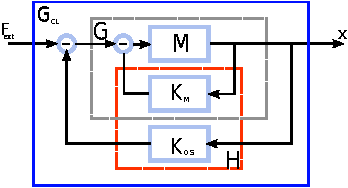
\includegraphics[width=15cm]{./figures/blocks_paper.pdf}
	\caption[Mechanical Oscillator and Feedback Systems]{Mechanical oscillator and feedback systems. The mechanical oscillator can be seen as plant ($G$) and the optical spring $K_{OS}$ as feedback or
	alternatively as free test mass (plant M) and $H=K_{OS}+K_M$ as feedback. 
	Both the cases lead to the same closed loop transfer function $G_{CL}$ which describes the system as a damped mechanical oscillator in presence of
	the optical spring, subjected to the external force $F_{ext}$ and corresponding displacement $x$ as output.}
	\label{fig:blocks2}
\end{figure}
In both cases we obtain the same closed-loop transfer function, equivalent to the one we would have obtained by
rewriting the equation of motion of a damped mechanical oscillator with an optical spring:
\begin{eqnarray}
\label{eqn:TFco}
G_{CL}=\frac{x}{F_{ext}}=\frac{G}{1+K_{OS} G}=\frac{M}{1+H M}\nonumber\\
=\frac{1}{-m\Omega^2+K_M+K_{OS}}%=\frac{1}{ms^2+b s+k_m}
\end{eqnarray}

The stability of the total system can again be evaluated  by either looking at the poles of the closed-loop
transfer function $G_{CL}$, or looking at the gain and phase margin of the open loop transfer function $OL_{MH}=-H/m\Omega^2$. The latter is generally more convenient. Unless compensated by large mechanical dissipation in $K_M$, the positive dynamic feedback for the statically stable case ($\delta>0$) leads to a dynamically unstable system. 
Intuitively this can be understood as a phase delay in the radiation pressure build-up which is caused by the cavity storage time.
For $\delta<0$ the system is statically unstable.

\subsection{Double Carrier Spring}

The seemingly intrinsic instability of optical springs can be overcome by a scheme 
proposed by Corbitt et al. \cite{Corbitt07}. The carrier is set at a large positive detuning ($\delta>0$, large $\delta/\gamma$). This provides a static restoring force, together with a relatively small dynamic instability (anti-damping). Then a sub-carrier is added at lower power and with a small negative detuning ($\delta<0$, small $|\delta|/\gamma$). The sub-carrier adds sufficient dissipation to stabilize the total optical spring, while leaving the sign of the static restoring force unchanged.
For appropriately chosen parameters of carrier ($c$) and sub-carrier ($sc$) (power $P_0^c$ and $P_0^{sc}$, detuning  $\delta_c$ and $\delta_{sc}$) the resulting total system thus becomes stable.

The spring constant of the total optical spring is simply the sum of the individual spring constants of the carrier and sub-carrier
\begin{eqnarray}
\label{eqn:KOSsum}
K_{OS}=K_{OS}^c+K_{OS}^{sc}
\end{eqnarray}
where the individual springs $K_{OS}^c$ and $K_{OS}^{sc}$ are given by equation \ref{eqn:TFco}.

%Fig.\ref{fig:stability} shows the stability of the trap-system at various values of  sub-carrier power and detuning for fixed carrier settings ($P_0^c=1~{\rm Watt}$, $\delta_c/\gamma = 2$) in our example system.

Conceptually we can think of the dual-carrier optical spring as a physical implementation of a feedback control filter for the mechanical system. With this tool at hand, we can start to analyze the behavior and stability of higher dimensional mechanical systems in the next section.

%\begin{figure}[htbp]
%	\centering
%		\includegraphics[width=9cm]{./images/KMKOSstability}
%	\caption{{Suspension stability region for different sub-carrier detuning ratio $\delta_{sc}/\gamma$ and input power values.
%	The carrier detuning ratio and its power have been set at $\delta_c/\gamma=2$ and $P0_c=1\,$W respectively. 
%	 At $\delta_{sc}/\gamma=0$ or $P0_{sc}=0\,$W only the carrier spring is effective and the system is not stable. The stability
%	 can be recovered only when the sub-carrier beam is injected into the cavity.}}
%	\label{fig:stability}
%\end{figure}


\section{Control model of longitudinal and angular degrees of freedom}
\label{sec:III} 

We will now extend our analysis to additional degrees of freedom. Experimentally, a torsion pendulum suspension is  easy to build. Therefore we will focus our attention to controlling the yaw motion of a test mirror, keeping in mind that the method can be applied to any additional degree of freedom. For actively controlling two degrees of freedom (length and yaw), we need a two-dimensional control system. In other words, we will need a second dual-carrier optical spring in a setup that for example looks like Fig.\ref{fig:angular}. We will label the two dual-carrier optical fields as beams $A$ and $B$. Each beam includes a carrier and a sub-carrier field, i.e.
\begin{eqnarray}
\label{eqn:beams}
\mbox{Beam A = carrier A + sub-carrier A}\\ \nonumber
\mbox{Beam B = carrier B + sub-carrier B}\nonumber
\end{eqnarray}
The two beams have a different optical axis, and each has its own optical spring constant, $K_{OS}^A$ and $K_{OS}^B$, given by equation 
\ref{eqn:KOSsum}.

If we define $x_A$ and $x_B$ as the longitudinal displacement of the mirror at the contact points
of beam A and beam B on the test mirror,
 %the position of the mechanical system at the attachment point of \tcr{incidence of} beam $A$ and beam $B$ \tcr{on the %test mirror}, 
 and $F_A$ and $F_B$ as the corresponding exerted forces, we can describe the mechanical system with a plant matrix $M$:
\begin{equation}
 \begin{pmatrix}
x_A\\ x_B
\end{pmatrix} 
=
M \begin{pmatrix}
F_{A}\\ F_{B}
\end{pmatrix}
\label{eq:MF}
\end{equation}
The explicit expression for $M$ for a torsion pendulum is given in appendix \ref{app:B}.

The control is provided by the optical springs. In the $x_A$-$x_B$ basis the control matrix $H$ is diagonal and given by  (also see Fig.\ref{fig:block_loops})
\begin{equation}
\begin{pmatrix}
F_{A}\\ F_{B}
\end{pmatrix}
= H
 \begin{pmatrix}
x_A\\ x_B
\end{pmatrix} 
=  \begin{pmatrix}
K_{OS}^A & 0 \\ 0 & K_{OS}^B
\end{pmatrix} 
 \begin{pmatrix}
x_A\\ x_B
\end{pmatrix} 
\label{eq:HX}
\end{equation}

\begin{figure}[t]
	\centering
		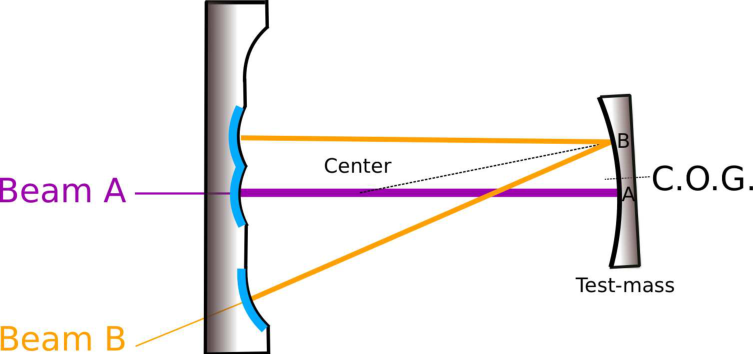
\includegraphics[width=15cm]{./figures/trap_drawing_paper2.pdf}
	\caption[Angular Trap Schematic]{
	In this sketch the main purple (Beam A) optical axis hits the test mirror %only slightly off-center 
	at point A, slightly displaced from the center of gravity (C.O.G.), such
	 that it still corresponds mainly to the length degree of freedom. Thus the second orange (Beam B) optical axis, which hits the test mirror closer to the edge at point B, needs much less power to balance the total DC torque. In our test setup the large input coupler is a composite mirror. It is 600 times more massive than the small mirror. The choice of a V-shaped beam B results in a more practical spot separation on the input coupler. }	


%with orders of magnitude more mass than the small mirror, 
%in order to ensure two different optical axes rigidly coupled.}	
	%can be as a multiple mirror.}%A monolithic, suspended platform is used for all auxiliary mirrors. %Once both one dimensional optical traps are engaged, i.e. their electrical feedback turned off, the DC alignment of the test mirror can still be adjusted by tuning \tcb{the...AOM frequency.}
	
	\label{fig:angular}
\end{figure}



\begin{figure}[htbp]
%	\centering
		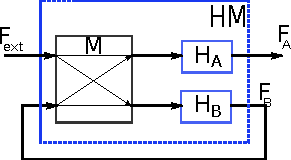
\includegraphics[width=15cm]{./figures/block_mimo_paper.pdf}
	\caption[Block Diagram of Optical Trap Beams]{Block diagram of beam A and beam B. The transfer function $F_A/F_{ext}$ is equal to $OL_A$ from equation \ref{eq:2dol}. Each loop affects the other resulting in cross terms
	present in the matrix $HM$. $M$ and $H_{A,B}$ are the transfer functions of the mechanical system and the optical springs of beam A and B, respectively.}
	\label{fig:block_loops}
\end{figure}

%\tcb{The model includes two optical cavities, referred to as beam A and B, both with an optical finesse of 104. 
%	The main cavity (beam A) is pumped with 0.8 Watt of carrier light, detuned by 36 kHz (blue detuning), and 0.2 
%	Watt of sub-carrier light, detuned by 12 kHz (red detuning). This produces a statically and dynamically stable 
%	optical spring with a lever arm of 1.3 mm, measured from the payload center of gravity. A second optical spring 
%	(beam B) is pumped with 16 times less power, but is otherwise similar to beam A. This side cavity has a lever 
%	arm of 2 cm on the payload, such that the DC radiation pressure torques of beam A and B cancel. The DC radiation 
%	pressure force is canceled by displacing the position pendulum.}

%\subsection{Method}
%\tcb{remove subsection}
For a multi-dimensional feedback system to be stable, it is sufficient that each individual (one-dimensional) feedback loop is stable, assuming all remaining control loops are closed. In other words, in our two-dimensional opto-mechanical system, we close the beam $B$ control filter for evaluating the open loop transfer functions $OL_{A}$, and vice versa. For the open loop transfer functions $OL_{A}$ and $OL_{B}$ we then find: 
\begin{eqnarray}
\label{eq:2dol}
OL_{A}=e_A^{T}\left(\mathds{1}-HM (\mathds{1} - e_A e_A^T) \right)^{-1}HMe_A  \\
OL_{B}=e_B^{T}\left(\mathds{1}-HM (\mathds{1} - e_B e_B^T) \right)^{-1}HMe_B \nonumber
\end{eqnarray}
with $e_A^T=(1,0)$ and $e_B^T=(0,1)$. The derivation of this expression is given in appendix \ref{app:C}.


%%%%%%%%%%%%%%%%%%%%%%%%%%%%%%%%%%%%%


\subsection{An Example}

It is worth considering a specific set of possible values for our model and evaluate the control of  angular and longitudinal degrees of freedom of a gram-scale test mirror using the radiation pressure of the light.
All the optical fields involved in our analysis are derived from the same wavelength light source through frequency shifting.
The model includes two optical cavities (Fig.\ref{fig:angular}), referred to as beam A and B, both with an optical finesse of  about $8000$ and linewidth $\gamma/(2 \pi) = 110\,$kHz. 
The main cavity (beam A) is pumped with $1\,$W of carrier light, detuned by $\delta/(2 \pi)= 250\,$kHz (blue detuning, $\delta/\gamma = 2$), and $0.2\,$W of sub-carrier light, detuned by $\delta/(2 \pi) =60\,$kHz (red detuning, $\delta/\gamma = -0.5$). This produces a statically and dynamically stable optical spring with a lever arm of $0.8\,$mm, measured from the payload center of gravity (C.O.G.). A second optical spring (beam B) is pumped with 6 times less power of carrier light, detuned by $=186\,$kHz (blue detuning, $\delta/\gamma=1.5$), and $40\,$mW of sub-carrier light, detuned by $60\,$kHz (red detuning, $\delta/\gamma=-0.5$). This side cavity has a lever arm of $3.3\,$mm on the payload, such that the DC radiation pressure torques of beam A and B cancel. The DC radiation pressure force can be canceled by displacing the position pendulum.

\begin{figure}[htbp]
	\centering
		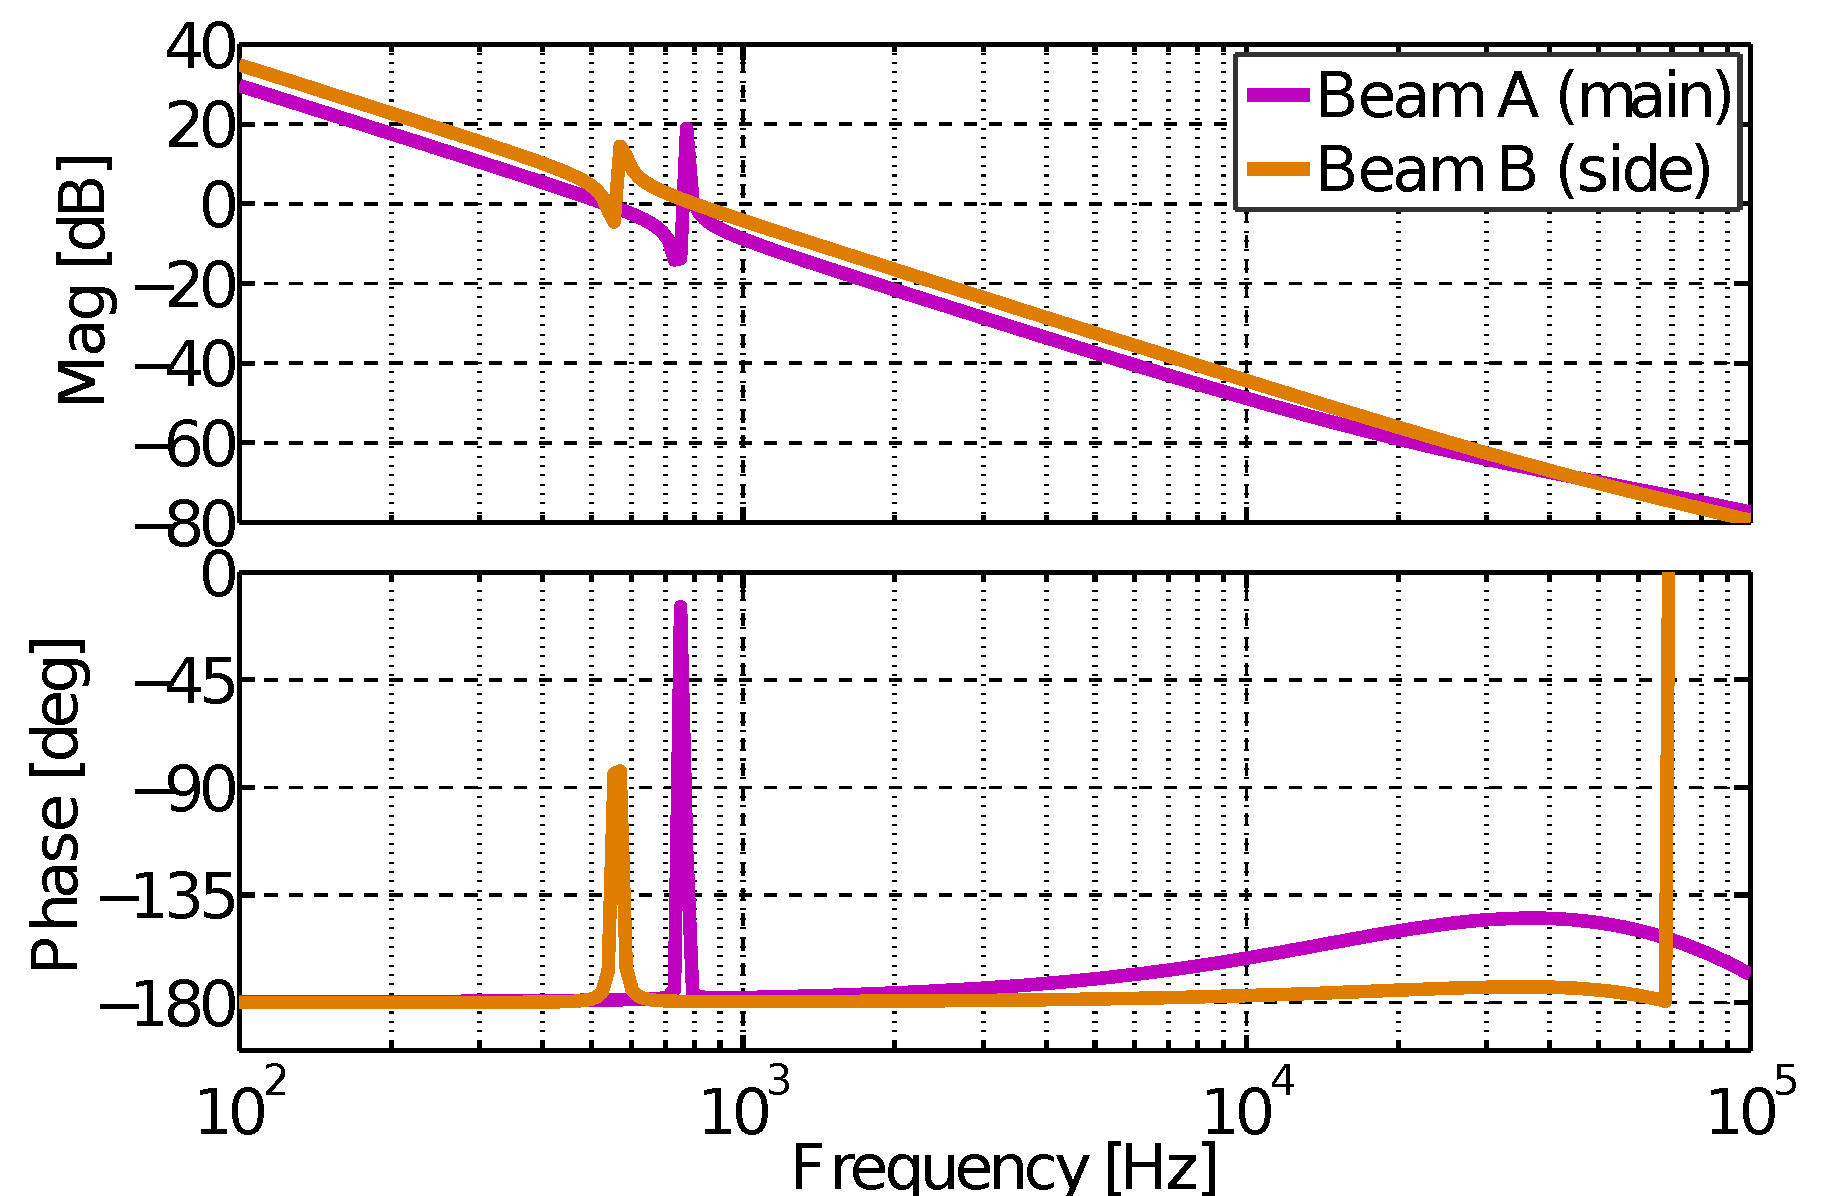
\includegraphics[width=15cm]{./figures/open_loops_TF_paper2.pdf}%filename.pdf}%
		%\includegraphics[width=8cm]{./images/filename.pdf}%
	\caption[Open Loop Gain for Optical Trap Cavities]{Open loop gain (OLG) for the main and side cavity.	The respective other loop is closed, and shows up as a resonance in the OLG. Note that, despite multiple unity gain crossings, both loops are stable because the resonances effectively implement a lead filter and the OLG avoids the critical point -1. Thus the dynamic interplay between multiple trapping beams on one payload does not introduce an instability.}
	\label{fig:control_loops}
\end{figure}


The stability of the combined two-dimensional system is addressed in Fig.\ref{fig:control_loops}. Plotted are the open loop gain functions of the two degrees of freedom (the two optical traps) under the assumption that the other loop is closed. The presence of the second loop introduces a resonance feature in each loop at the unity gain frequency of the other loop. However the open loop gain avoids the critical point -1 (phase at zero), leading to a stable system. The model parameters were intentionally tuned for low damping / high quality factor in order to demonstrate that the system remains stable. Lower quality factors, and therefore stronger cooling is easily achievable.

%If we consider the cavity with both loops closed and we scan one of the mirror we obtain the stability region showed
%in Fig.\ref{fig:stability_region}. The green shaded area represents the offset range of the cavity length at which the two loops remain still stable. The range is $\backsim 20\,$pm.
%
%\begin{figure}[htbp]
%	\centering
%		\includegraphics[width=9cm]{./images/DC_offset}
%	\caption{{(Left) Static carrier and sub-carrier build-up as function of mirror position: Plotted are carrier and sub-carrier build-up (calibrated in Newton of radiation pressure) as a function of the respective cavity position. Also shown in blue is the total force. The trap is both statically and dynamically stable in the green shaded area.
%	%In Figure 4 the static (DC) radiation pressure force due to each of the four laser fields is plotted 
%%as a function of cavity position. Indicated by green shading are the regions with a stable optical 
%%spring (statically and dynamically). 
%With the chosen model parameters those regions are about 
%20 picometers wide.}}
%	\label{fig:stability_region}
%\end{figure}


\subsection{Stability range}
\label{sec:stability}
%\input{OT_paper_stabrange.tex}
We can now estimate the robustness of our feedback control system 
by changing the microscopic length $\delta x_A$ and $\delta x_B$ of the two cavities. This changes the detuning of the optical springs for both beams. Therefore the propagators $X_A$ and $X_B$ for both beams change according to $X_{A,B}=r_1r_2 e^{-i\delta_{A,B}\tau_{A,B}}\cdot e^{ik\delta x_{A,B}}$. For each position both the static and dynamical stability of the total optical spring system given by equation \ref{eq:2dol}
%s \ref{KOS_full_2}, \ref{eqn:K0} and \ref{eqn:KOSsum}
is reevaluated.
%For beam A (and similarly for beam B) we correct the optical spring introducing the additional $\delta x$ to the propagator $X$, becoming $X=r_1r_2 e^{-i\delta\tau}\cdot e^{ik\delta x}$, the optical springs for both beams $i=A,B$ become
%\begin{eqnarray}
%\label{eqn:Koffset}
%K_{OS}^i = K_{OS}^{c_i} + K_{OS}^{sc_i} \approx -2 \eta r_1r_2 \tau(\delta_c+\delta_{sc})k\delta x 
%K_{OS}^B = K_{OS}^{cB} + K_{OS}^{scB} \approx -2 \eta r_1r_2 \tau(\delta_c+\delta_{sc})k\delta x
%\end{eqnarray}
%and we check the stability with the same procedure described in Section(bla) at different values of the offset. 
%at each single value of the cavity lengths. 

In Fig. \ref{fig:stability_region} the radiation pressure force due to the intra-cavity power of both beams
versus the cavity offset is shown. The green shaded area represents the position range in which the two loops remain stable.  The range is $\backsim 20\,$pm. 
The DC force fluctuations that the system can tolerate are given by the y-axis interval that the blue curve spends in the green shaded area. %{\color{red} The range is about $xx N$ for beam A and about $yy N$ for beam B. }

\begin{figure}[htbp]
	\centering
		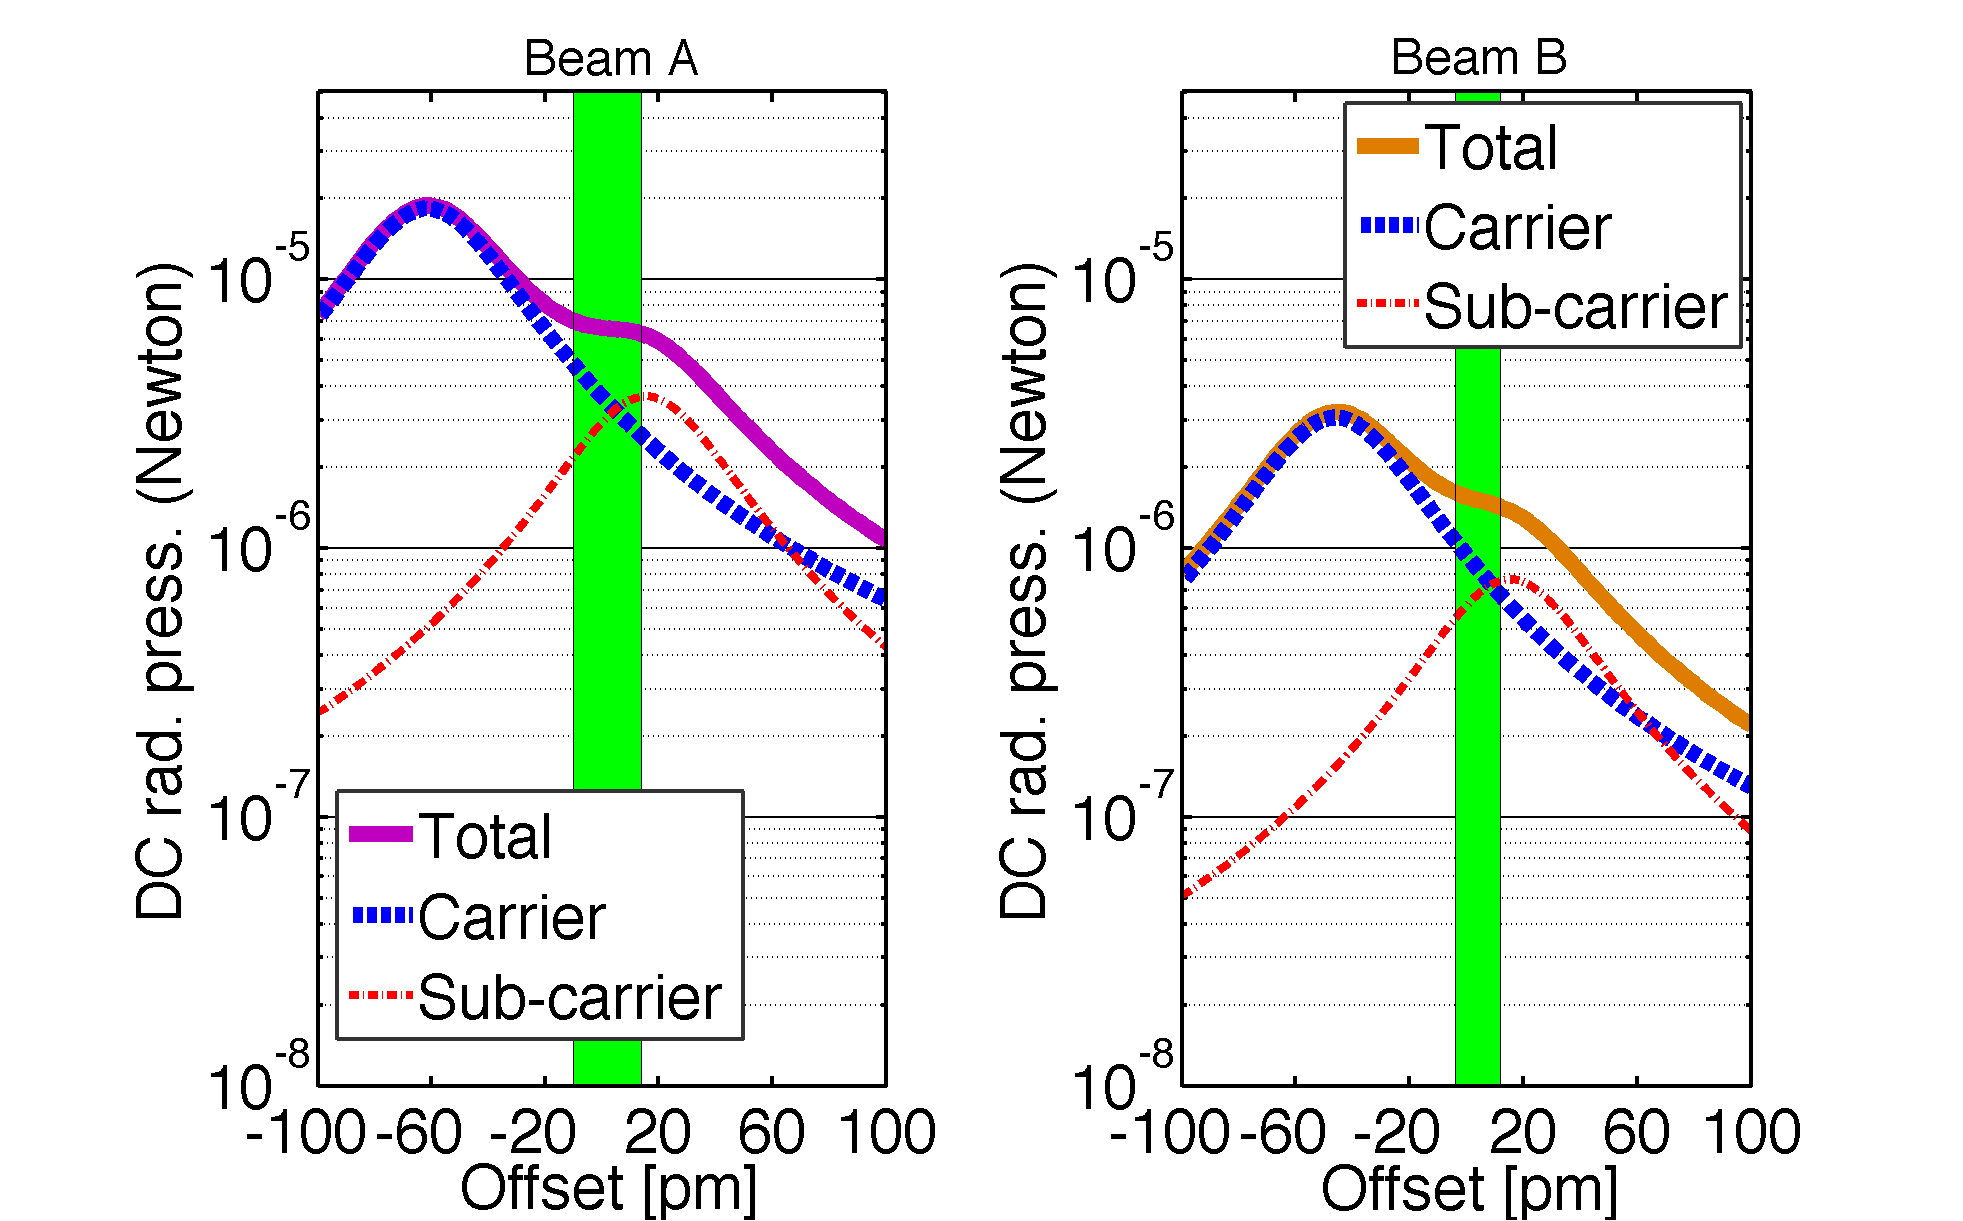
\includegraphics[width=15cm]{./figures/DC_offset_paper3.pdf}
	\caption[Stable Optical Spring Detuning Range]{Static carrier and sub-carrier build-up (calibrated in radiation pressure force) as a function of the respective cavity position. Also shown in blue is the total radiation pressure force. Using the stability testing method from section \ref{sec:stability} we find that the trap is both statically and dynamically stable in the green shaded area.
	%In Figure 4 the static (DC) radiation pressure force due to each of the four laser fields is plotted 
%as a function of cavity position. Indicated by green shading are the regions with a stable optical 
%spring (statically and dynamically). 
With the chosen model parameters those regions are about 
20 picometers wide.}
	\label{fig:stability_region}
\end{figure}

%\tcb{Finally, Fig...... shows a simple noise budget for this MATLAB model. It is calibrated in actual motion after the trap closed loop gain suppression. The seismic noise estimate is based on a typical ground motion filtered by a one-stage passive isolation platform with a resonance frequency of $1\,$Hz. It results in a residual RMS motion of about 1 picometer. This is smaller than the 12 picometer stability band shown in Figure 4. Therefore it should be possible to turn off any feedback to the cavity length or laser frequency. The two cavities will remain locked purely due to the radiation pressure trapping force, thus trapping the payload.}


\section{Angular instability}
\label{sec:IV} 
When operated with high intracavity laser power, suspended Fabry-Perot cavities like the arm cavities of LIGO have a well known angular instability. It  arises from coupling the misalignment of the two cavity mirrors to radiation pressure torques. This is known as the Sidles-Sigg instability \cite{Sidles06}. In this section we show that the intrinsic strength of an optical trap for alignment degrees of freedom is generally bigger, i.e. has a bigger spring constant than any associated Sidles-Sigg instability. 

We start with a cavity of length $L$, with $x_1,x_2$  being the position of the beam spots on mirrors 1 and 2. $\theta_1,\theta_2$ are the yaw angles of the two mirrors, and $R_1,R_2$ are their radii of curvature. The corresponding g-factors are $g_{1,2}=1-L/R_{1,2}$.
If one or both of the mirrors are slightly misaligned ($\theta_{1,2}\neq 0$), then the radiation pressure force exerts torques $T_1$ and $T_2$ on the two mirrors, given by the following relation (see for instance \cite{Sidles06} or \cite{Ballmer13}): 
\begin{equation}
\label{SidlesSigg_Basic}
\left(
\begin{array}{c}
T_1\\
T_2
\end{array}
\right)
=
\frac{F_0 L}{1-g_1 g_2}
\left(
\begin{array}{cc}
g_2 & -1\\
-1 & g_1
\end{array}
\right)
\left(
\begin{array}{c}
\theta_1\\
\theta_2
\end{array}
\right)
\end{equation} 
with $F_0=P_0\frac{t_1^2}{(1-X)(1-\overline{X})} \frac{2 r_2^2}{c}$ being the intra-cavity radiation pressure force. Sidles and Sigg first pointed out that, since the determinant of the matrix in this equation
%\ref{SidlesSigg_Basic}
 is negative, the two eigenvalues have opposite sign. This always leads to one stable and one unstable coupled alignment degree of freedom.

First we note that for a situation in which one mass is sufficiently heavy that we can neglect any radiation pressure effects on it (i.e. $\theta_1=0$), it is sufficient to choose a negative branch cavity (i.e. $g_1<0$ and $g_2<0$) to stabilize the setup. This is for instance the case for the example setup described in Fig. \ref{fig:angular}.

Next we want to compare the order of magnitude of this effect to the strength of an angular optical spring. If we call $h$ the typical distance of the beam spot from the center of gravity of the mirror, and $x$ the cavity length change at that spot, the order of magnitude of the optical spring torque is:
\begin{eqnarray}
%F=K_{0}\cdot x = T/h\approx \frac{F_0L}{h}\cdot \frac{x}{h}
T\approx \frac{F_0 L}{1-g_1g_2}\cdot \frac{x}{h}
\end{eqnarray}
We can express this as the strength of an optical spring located at position $h$. The corresponding spring constant $K_{SS} \approx T/(h x)$. Thus we can see that
\begin{eqnarray}
\label{eqn:KSS_def}
K_{SS} \approx \frac{F_0}{1-g_1g_2}\cdot \frac{L}{h^2}.
\end{eqnarray}
We now consider the adiabatic optical spring ($\Omega=0$) in equation \ref{eqn:K0}.  Expressed in terms of $F_0$, $K_{OS}$ becomes
\begin{eqnarray}
\label{eqn:KOS_exact}
K_{OS}=i F_0 \frac{X-\overline{X}}{(1-X)(1-\overline{X})}   2 k
\end{eqnarray}
Since we operate near the maxium of the optical spring, the order of magnitude of the resonance term can be estimated as
\begin{eqnarray}
\label{eqn:res_est}
\frac{X-\overline{X}}{(1-X)(1-\overline{X})} \approx \frac{-i}{1-|X|}
\end{eqnarray}
Thus we can estimate the magnitude of  $K_{OS}$ as
\begin{eqnarray}
\label{eqn:K0_order}
K_{OS} \approx F_0 \frac{4\pi}{\lambda}\frac{1}{1-|X|} \approx F_0 \frac{4}{\lambda} \mathcal{F}
\end{eqnarray}
where $\mathcal{F}$ is the cavity finesse.
From equations \ref{eqn:KSS_def} and \ref{eqn:K0_order} we see that the optical spring $K_{OS}$  is much larger than the Sidles-Sigg instability spring $K_{SS}$ if
\begin{eqnarray}
\label{eqn:h2}
h^2 >> \frac{\lambda L}{\pi} \frac{1}{1-g_1 g_2} \frac{\pi}{4 \mathcal{F}}
\end{eqnarray}
Now recall that the beam spot size in a Fabry-Perot cavity is given by \cite{Siegman86}
\begin{equation}
w_1^2 = \frac{\lambda L}{\pi} \sqrt{\frac{g_2}{g_1(1-g_1 g_2)}}
\label{equ:spotsize1}
\end{equation} 
Assuming a symmetric cavity ($g_1=g_2$) for simplicity, we thus find that $K_{OS}$  dominates over $K_{SS}$ if
\begin{eqnarray}
\label{eqn:h2w}
h^2 >> w_{1,2}^2 \frac{1}{\sqrt{1-g_1 g_2}} \frac{\pi}{4 \mathcal{F}}
\end{eqnarray}
This condition is naturally fulfilled since we need to operate the angular optical spring with separate beams ($h>w_{1,2}$) and a large finesse ($\mathcal{F}>>1$). Therefore the angular optical spring is indeed strong enough to stabilize the Sidles-Sigg instability.

\section{Radiation Pressure Noise}
\label{sec:V}
Another advantage of radiation pressure control, compared to a classical approach based on photo detection and feedback, is its fundamental noise limit. Unlike in the classical approach, the shot noise and other sensing noises %from detecting a potentially small sample of the beam 
never enter a radiation-pressure-based feedback loop. Even though technical laser noise is typically bigger in the simple cavity setup discussed in this paper, the only fundamental noise source of the scheme is quantum radiation pressure noise. In this section we give the full expression for radiation pressure noise in the case of a dual-carrier stable optical spring.

First, we note that as long as we are interested in frequencies much smaller than the any of the features in the detuned cavity transfer function, the radiation pressure noise is relatively simple. If we also assume that the end mirror has a reflectivity of 1, the one-sided ($f\ge0$) radiation-force amplitude spectral noise density is given by
\begin{eqnarray}
\label{eqn:simpleRPN}
S_F (f) = \frac{2}{c} G \sqrt{2 \hbar \omega P_{\rm in}}
\end{eqnarray}
where $G$ is the power gain of the cavity in the detuned configuration, and $P_{\rm in}$ is the power of the shot noise limited beam entering the cavity.
Equation \ref{eqn:simpleRPN} is valid for carrier and subcarrier separately.
Note that this equation does not hold if the end mirror has a finite transmissivity, as quantum fluctuations entering from that port will also contribute to the intra-cavity shot noise. In the case of a critically coupled cavity, this will result in an increase of the intra-cavity radiation-force amplitude spectral noise density by exactly a factor of 2.

To calculate the exact expression for the radiation pressure noise induced cavity fluctuations, we first realize that we can calculate the radiation-force amplitude spectral noise for a static cavity, and then compute the response of the dual-carrier optical spring system to that driving force. This yields the correct answer up to first order in the size of the quantum fluctuations. For the calculation we track the quantum vacuum fluctuations entering at both ports of the cavity. It is useful to introduce a function $F$:
\begin{eqnarray}
\label{eqn:RPNfunction}
F(f) = F\left(\frac{\Omega + \delta + \omega_{res}}{2 \pi}\right) =& \frac{1}{1-XY^2}  \\ =& \frac{1}{1-r_1r_2e^{-2 i \delta\tau}e^{-2 i \Omega\tau}}
\end{eqnarray}
The amplitude build-up factors for fluctuations at frequency $f$ entering through the input coupler (1) and the end mirror (2) thus are
\begin{eqnarray}
\label{eqn:RPNfunction12}
 t_1 F(f) \,\,\, {\rm and} \,\,\ r_1 t_2 F(f), 
\end{eqnarray}
where we already dropped the one-way propagation factor because it drops out in the radiation force noise calculation below. 
We can now introduce the notation $F_0=F(f_0)$, $F_+=F(f_0+f)$ and $F_-=F(f_0-f)$. We then get the following expression for the one-sided radiation-force power spectral density for either carrier or sub-carrier.
\begin{eqnarray}
\label{eqn:RPN_P}
S_F (f) = \frac{2}{c} S_P (f) \,\,\,\,\,\, {\rm and}
\end{eqnarray}
\begin{eqnarray}
\label{eqn:RPN}
|S_P (f)|^2 =   \hbar \omega P_0 t_1^2|F_0|^2 (t_1^2 \!\!+\! r_1^2t_2^2)( |F_+|^2 \!\!+\!  |F_-|^2)
\end{eqnarray}
Here $P_0$ is the entering carrier power, and $f_0$ is its frequency. We can see that we recover equation \ref{eqn:simpleRPN} in the limit $t_2 \rightarrow 0$ and $G/t_1^2=|F_0|^2=|F_+|^2=|F_-|^2$. The resulting force noise from carrier and sub-carrier for the cavity A in the example above is plotted in Fig.\ref{fig:RFASD} (\emph{top}).
\begin{figure}[htbp]
	\centering
		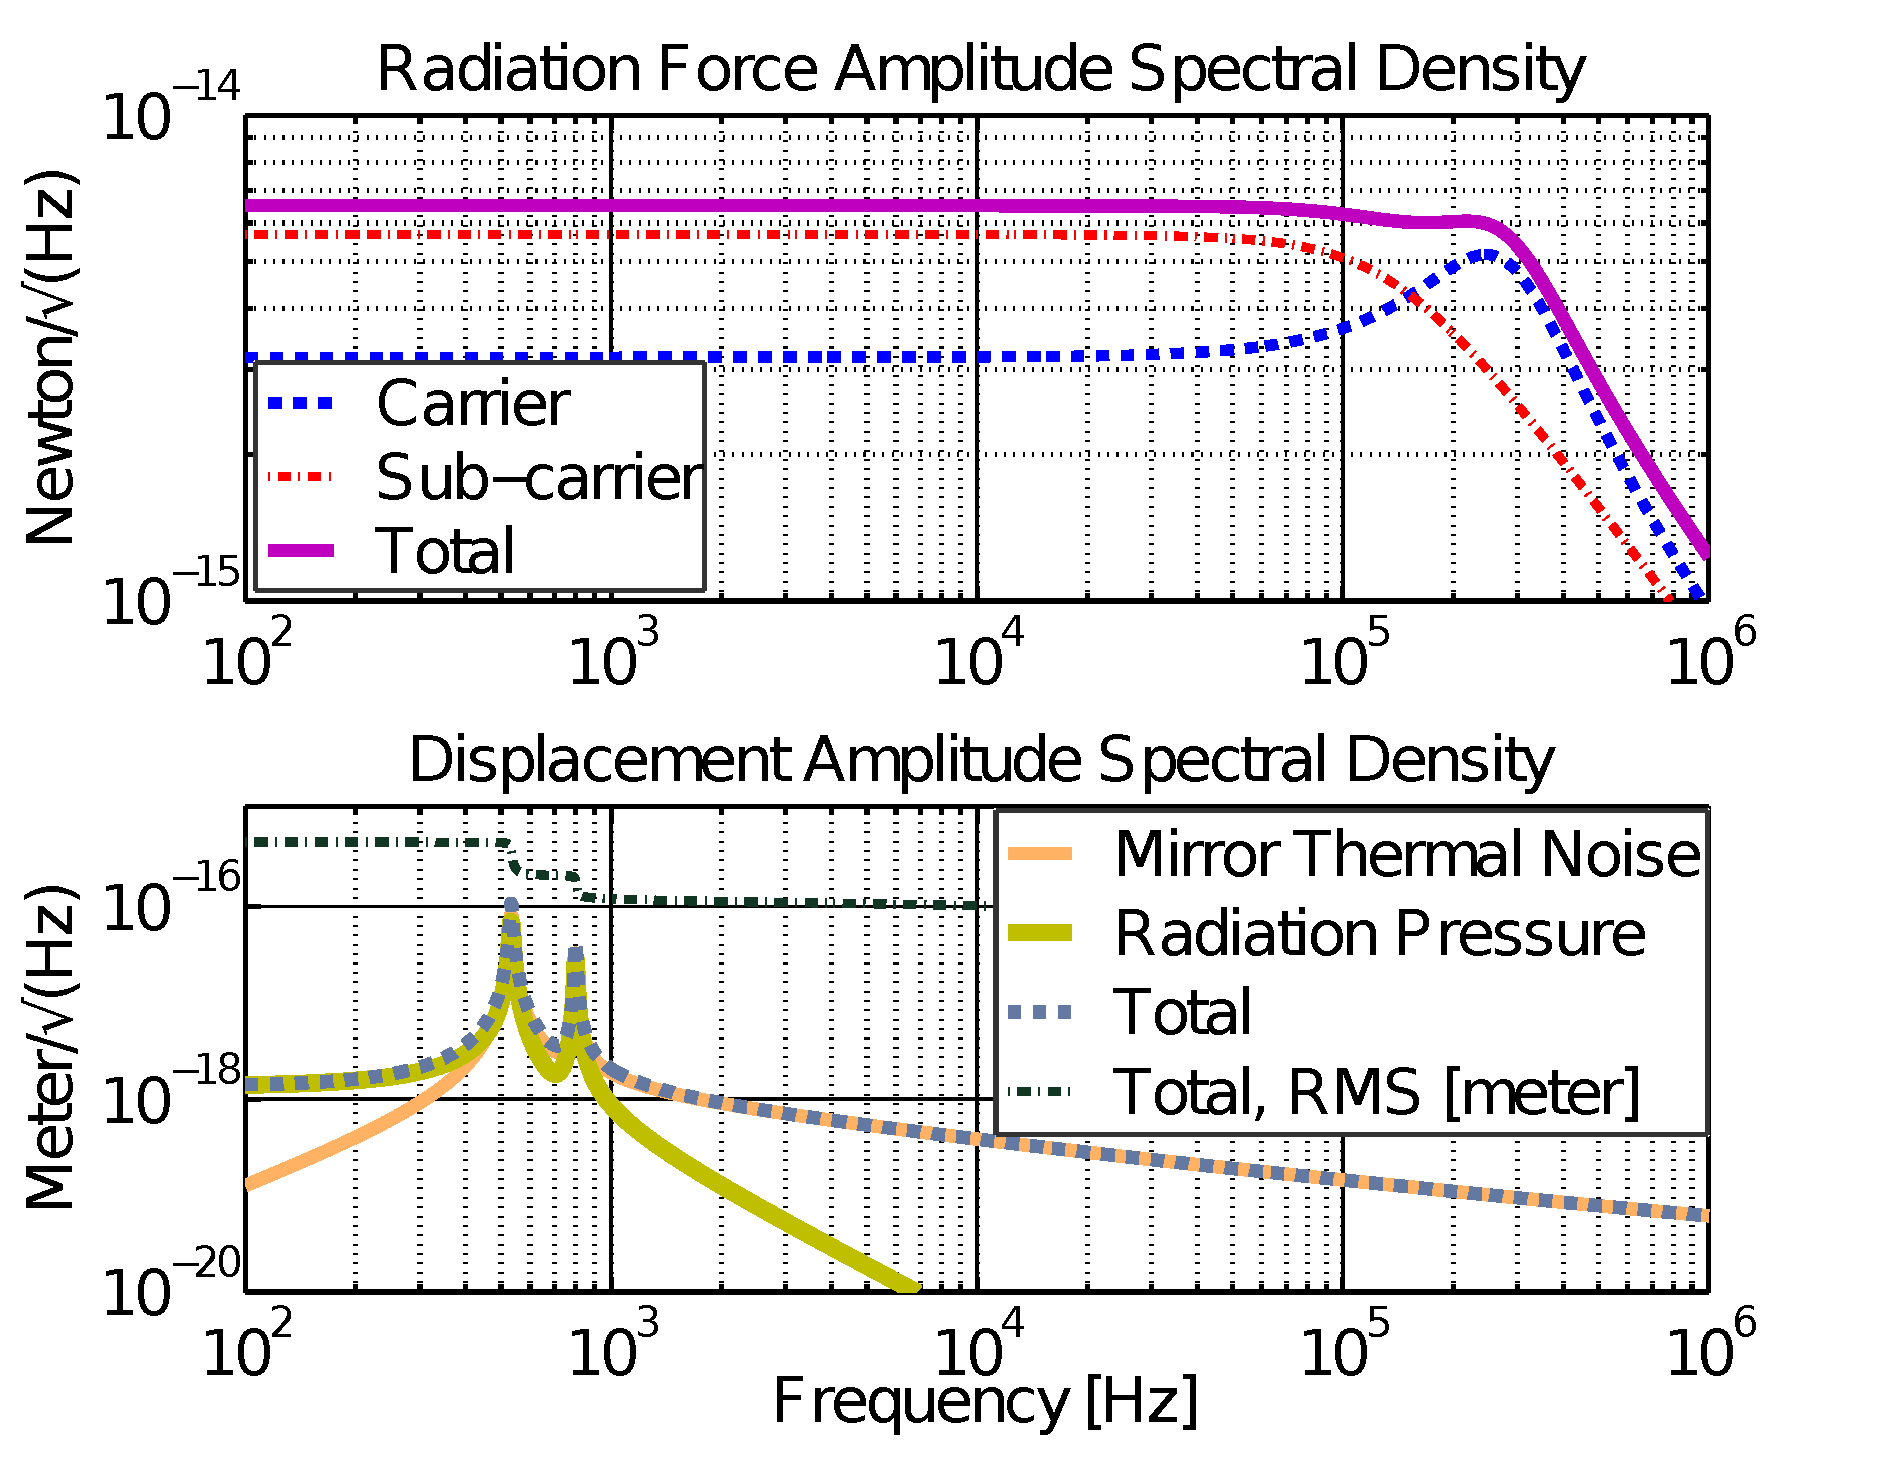
\includegraphics[width=15cm]{./figures/trap_radPresA_paper2.pdf}
	\caption[Radiation Force Amplitude Spectral Density]{(\emph{Top}) Radiation force amplitude spectral density for the dual-carrier optical spring used in beam A of the above example. The sub-carrier dominates the noise at low frequency, but the higher-power carrier contributes more at high frequencies. Also note that if we choose the same free spectral range for the two carriers, there would be an additional beat note at the difference frequency of $310~{\rm kHz}$. (\emph{Bottom})  Radiation pressure and thermal noise displacement amplitude spectral density. The radiation pressure noise is calculated using the opto-mechanical response given in equation \ref{eqn:closedloop_tf}. The thermal noise is based on a theoretical calculation described in \cite{Saulson90}, \cite{Ballmer13}. Since seismic and suspension thermal noise depend on the experimental implementation, they are not shown, but they would also be suppressed by the optical spring closed loop response. The residual RMS motion due to the shown noise sources is less than $10^{-3}$ picometer. With the total RMS motion smaller than the 20 picometer stability band shown in Fig.\ref{fig:stability_region}, the two cavities will remain locked purely due to the radiation pressure trapping force.}
	\label{fig:RFASD}
\end{figure}

Next we calculate the response of the coupled opto-mechanical system to this driving force, using the following closed loop transfer function obtained from equations \ref{eq:MF} and \ref{eq:HX}:

\begin{eqnarray}
\label{eqn:closedloop_tf}
x = {M}({1-HM})^{-1}F
\end{eqnarray}

Above the optical spring resonances this leads to a $1/f^2$ fall-off of the displacement noise, as expected for radiation pressure noise. Meanwhile below the resonance, due to the closed loop suppression, we will have a flat displacement noise. %at a level of $S_x(f) ~ S_F(f)/K_{OS}$. 
Fig.\ref{fig:RFASD} bottom illustrates this in the case of the two-dimensional angular trap discussed above.

Finally we compare the resulting displacement noise to a classical photo-detection feedback control scheme with similar control bandwidth and control loop shape. If such a system is able to detect all availabe power and has no other dominating sensing noise sources, it can at best achieve a shot noise sensitivity of 
\begin{eqnarray}
\label{eqn:classyShot}
S_x \backsim \frac{l}{P_0}\sqrt{2 \hbar \omega P_0}
\end{eqnarray}
where $l$ is the cavity line width in meters. To have the same control bandwidth and loop shape the system needs a controller transfer function equal to the optical spring, $H = K_{OS} \backsim \frac{2 G P_0}{c l}$, and hence it will have a  noise performance similar to equation \ref{eqn:simpleRPN},  $H S_x=S_F$.  
Thus we find that the traditional control scheme can only achieve similar noise if all the power from the cavity is detected, and there are no other relevant sensing noise sources. 

%\section{TBD...NOISE?}
%Here I put some calculation made together with Stefan...(no text yet)
%\begin{eqnarray}
%E_{tot}=E_{0}^{tot} \left [1 + \alpha_+ e^{i\Omega t} E_+^{tot} +  \alpha_-^* e^{-i\Omega t} E_-^{tot}  \right ]
%\end{eqnarray}
%with
%\begin{eqnarray}
%\alpha^+= \frac{(a + i\phi)}{2}  \quad \mbox{and} \quad  \alpha^-= \frac{(a - i\phi)}{2}
%\end{eqnarray}
%where $a$ and $\phi$ are both complex numbers (is that necessary????).
%Recalling that:
%\begin{eqnarray}
%E_0^{tot}=t \frac{E}{1-X}, 
%X=r_1r_2e^{-ikL}, \\
%X_\pm=r_1r_2e^{-1K_\pm L}
%\end{eqnarray}
%we have
%\begin{eqnarray}
%E_{tot}=\frac{E_0t}{1-X}\left [ 1 +  \alpha_+' e^{i\Omega t}  +\alpha_-^{'*} e^{-i\Omega t}  \right ]
%\end{eqnarray}
%with
%\begin{eqnarray}
%\alpha_+' =  \frac{1-X}{1-X_+}\alpha_+ \quad \mbox{and} \quad \alpha_-^{'*} = \frac{1-X}{1-X_-} \alpha_-^* 
%\end{eqnarray}



\section{Conclusions}
In conclusion, we investigated the use of the radiation pressure of the laser light as an alternative to a conventional feedback system for controlling the 
longitudinal and angular degree of freedom of a mirror.
The method is based on a double dual-carrier scheme, using a total of four detuned laser fields in two cavities. 
The two dual-carrier beams hit the mirror in separate spots, forming two stable optical springs.
%Each dual-carrier beam hits the test mirror in two different spots, trapping the mirror in these two points. 
This constrains both the longitudinal and the angular degrees of freedom of the mirror, replacing completely the commonly used electronic feed-back system.
%We propose a system with two longitudinal traps acting on different spots of a single mirror; together, these traps will constrain both the position and one angular degrees of freedom of the mirror. This essentially replaces the magnetic drives with optical traps. The idea is promising and will be easy to apply to additional angular degree of freedom as well.
We showed that this setup allows a stable control of the two degrees of freedom, within a displacement range of the test mirror of $\sim 20\,$pm. This promising idea can be extended to the other angular degree of freedom.
We found that such a method creates an angular optical spring stronger than the angular Sidles-Sigg instability, which drives the requirement for angular control in the high power arm cavities of gravitational wave detectors. We also showed that the fundamental limit of this scheme is the quantum radiation pressure noise, resulting in a reduction in control noise compared to a conventional active feedback approach. 
%\tcr{This is a promising idea easily to extend to other degrees of freedom.}
We are working towards the experimental demonstration of this effect for a gram-scale mirror and beginning to explore its extension
to large-scale gravitational wave detectors.
%\tcb{Shall we talk about FIG.\ref{fig:stability_region}}


%Inline math may be typeset using the \verb+$+ delimiters. Bold math
%symbols may be achieved using the \verb+bm+ package and the
%\verb+\bm{#1}+ command it supplies. For instance, a bold $\alpha$ can
%be typeset as \verb+$\bm{\alpha}$+ giving $\bm{\alpha}$. Fraktur and
%Blackboard (or open face or double struck) characters should be
%typeset using the \verb+\mathfrak{#1}+ and \verb+\mathbb{#1}+ commands
%respectively. Both are supplied by the \texttt{amssymb} package. For
%example, \verb+$\mathbb{R}$+ gives $\mathbb{R}$ and
%\verb+$\mathfrak{G}$+ gives $\mathfrak{G}$
%
%In \LaTeX\ there are many different ways to display equations, and a
%few preferred ways are noted below. Displayed math will center by
%default. Use the class option \verb+fleqn+ to flush equations left.
%
%Below we have numbered single-line equations; this is the most common
%type of equation in \textit{Physical Review}:
%\begin{eqnarray}
%\chi_+(p)\alt{\bf [}2|{\bf p}|(|{\bf p}|+p_z){\bf ]}^{-1/2}
%\left(
%\begin{array}{c}
%|{\bf p}|+p_z\\
%px+ip_y
%\end{array}\right)\;,
%\\
%\left\{%
% \openone234567890abc123\alpha\beta\gamma\delta1234556\alpha\beta
% \frac{1\sum^{a}_{b}}{A^2}%
%\right\}%
%\label{eq:one}.
%\end{eqnarray}
%Note the open one in Eq.~(\ref{eq:one}).
%
%Not all numbered equations will fit within a narrow column this
%way. The equation number will move down automatically if it cannot fit
%on the same line with a one-line equation:
%\begin{equation}
%\left\{
% ab12345678abc123456abcdef\alpha\beta\gamma\delta1234556\alpha\beta
% \frac{1\sum^{a}_{b}}{A^2}%
%\right\}.
%\end{equation}
%
%When the \verb+\label{#1}+ command is used [cf. input for
%Eq.~(\ref{eq:one})], the equation can be referred to in text without
%knowing the equation number that \TeX\ will assign to it. Just
%use \verb+\ref{#1}+, where \verb+#1+ is the same name that used in
%the \verb+\label{#1}+ command.
%
%Unnumbered single-line equations can be typeset
%using the \verb+\[+, \verb+\]+ format:
%\[g^+g^+ \rightarrow g^+g^+g^+g^+ \dots ~,~~q^+q^+\rightarrow
%q^+g^+g^+ \dots ~. \]
%
%
%\subsection{Multiline equations}
%
%Multiline equations are obtained by using the \verb+eqnarray+
%environment.  Use the \verb+\nonumber+ command at the end of each line
%to avoid assigning a number:
%\begin{eqnarray}
%{\cal M}=&&ig_Z^2(4E_1E_2)^{1/2}(l_i^2)^{-1}
%\delta_{\sigma_1,-\sigma_2}
%(g_{\sigma_2}^e)^2\chi_{-\sigma_2}(p_2)\nonumber\\
%&&\times
%[\epsilon_jl_i\epsilon_i]_{\sigma_1}\chi_{\sigma_1}(p_1),
%\end{eqnarray}
%\begin{eqnarray}
%\sum \vert M^{\text{viol}}_g \vert ^2&=&g^{2n-4}_S(Q^2)~N^{n-2}
%        (N^2-1)\nonumber \\
% & &\times \left( \sum_{i<j}\right)
%  \sum_{\text{perm}}
% \frac{1}{S_{12}}
% \frac{1}{S_{12}}
% \sum_\tau c^f_\tau~.
%\end{eqnarray}
%\textbf{Note:} Do not use \verb+\label{#1}+ on a line of a multiline
%equation if \verb+\nonumber+ is also used on that line. Incorrect
%cross-referencing will result. Notice the use \verb+\text{#1}+ for
%using a Roman font within a math environment.
%
%To set a multiline equation without \emph{any} equation
%numbers, use the \verb+\begin{eqnarray*}+,
%\verb+\end{eqnarray*}+ format:
%\begin{eqnarray*}
%\sum \vert M^{\text{viol}}_g \vert ^2&=&g^{2n-4}_S(Q^2)~N^{n-2}
%        (N^2-1)\\
% & &\times \left( \sum_{i<j}\right)
% \left(
%  \sum_{\text{perm}}\frac{1}{S_{12}S_{23}S_{n1}}
% \right)
% \frac{1}{S_{12}}~.
%\end{eqnarray*}
%
%To obtain numbers not normally produced by the automatic numbering,
%use the \verb+\tag{#1}+ command, where \verb+#1+ is the desired
%equation number. For example, to get an equation number of
%(\ref{eq:mynum}),
%\begin{equation}
%g^+g^+ \rightarrow g^+g^+g^+g^+ \dots ~,~~q^+q^+\rightarrow
%q^+g^+g^+ \dots ~. \tag{2.6$'$}\label{eq:mynum}
%\end{equation}
%
%\paragraph{A few notes on \texttt{tag}s} 
%\verb+\tag{#1}+ requires the \texttt{amsmath} package. 
%Place the \verb+\tag{#1}+ command before the \verb+\label{#1}+, if any. 
%The numbering produced by \verb+\tag{#1}+ \textit{does not affect} 
%the automatic numbering in REV\TeX; 
%therefore, the number must be known ahead of time, 
%and it must be manually adjusted if other equations are added. 
%\verb+\tag{#1}+ works with both single-line and multiline equations. 
%\verb+\tag{#1}+ should only be used in exceptional cases---%
%do not use it to number many equations in your paper. 
%Please note that this feature of the \texttt{amsmath} package
%is \emph{not} compatible with the \texttt{hyperref} (6.77u) package.
%
%Enclosing display math within




%\begin{acknowledgments}
%We would like to thank Peter Saulson, Prayush Kumar, Riccardo Penco and Matt West for the many fruitful discussions. This work was supported by the National Science Foundation grant PHY-1068809. This document has been assigned the LIGO Laboratory document number  LIGO-P1300224.
%\end{acknowledgments}

%\appendix
%\section{Optical spring constant derivation}
\label{app:A} 
%\subsection{Optical spring constant}
%\label{sec:Apx1}

In this section we consider the effect of light stored in a detuned Fabry-Perot cavity using a classical approach.
The intra-cavity power generates radiation pressure that exerts on the cavity mirror a force $F_{rad}=-K_{OS}\cdot x$,
where $x$ is the mirror displacement and $K_{OS}$ is the optical spring constant.
Here we show the full derivation of the optical spring constant $K_{OS}$.

We consider a suspended Fabry-Perot cavity of length $L_0$ %shined by a laser light 
with an incident beam of wavelength $\lambda$ and power $P_0$.
First we calculate a general expression of the intra-cavity power and then its  radiation pressure force exerted on the end mirror.\\


\begin{figure}[htbp]
	\centering
		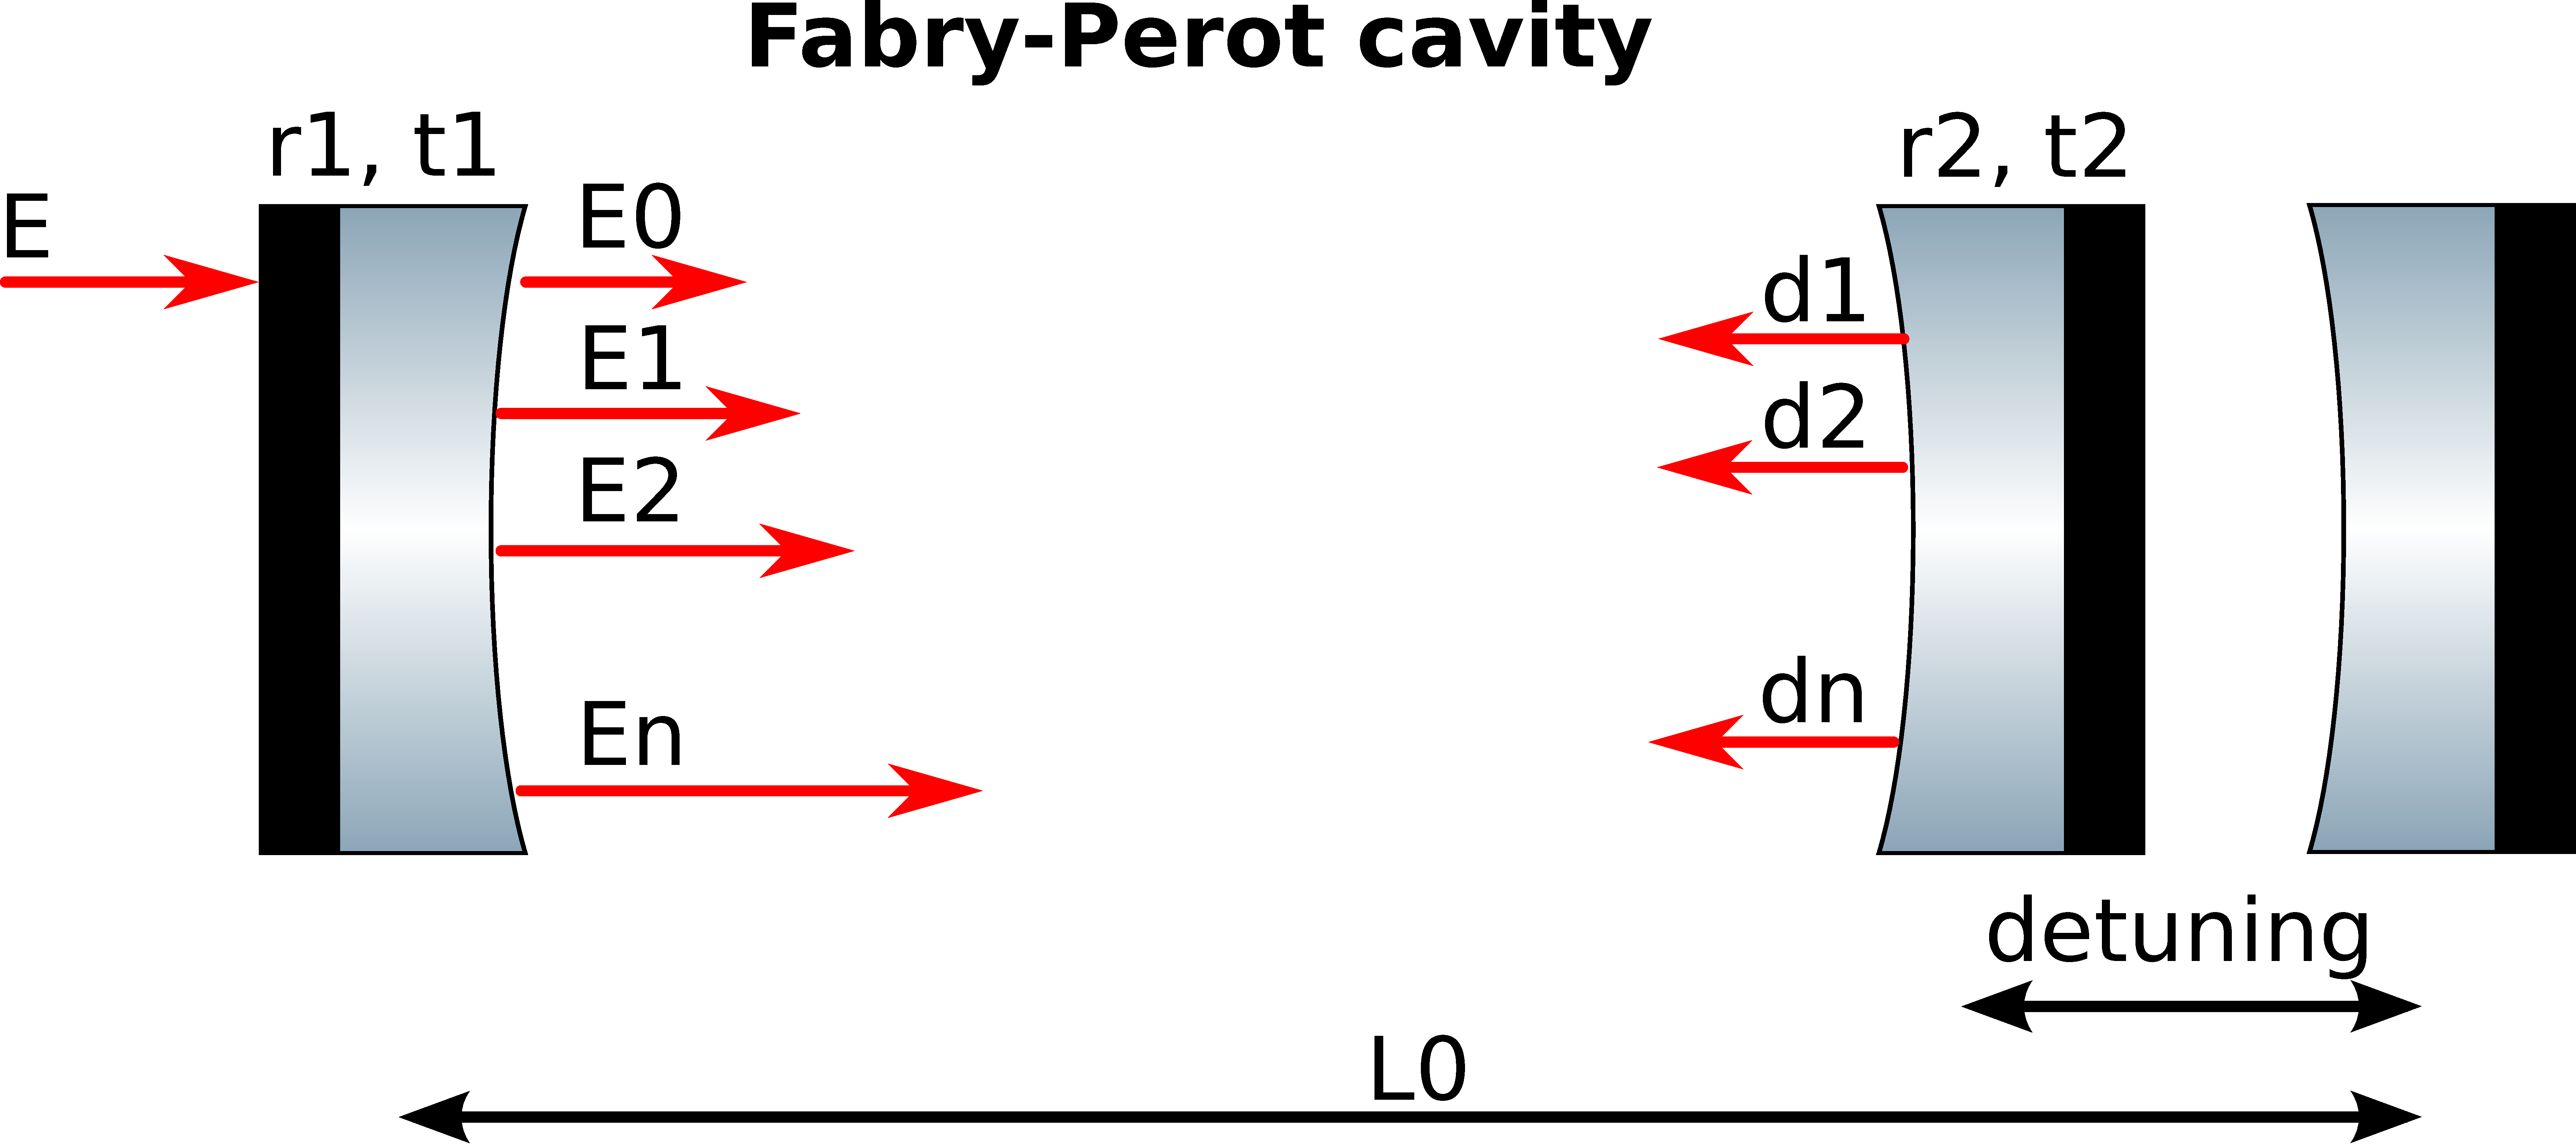
\includegraphics[width=8cm]{./images/cavity_paper.pdf}
	\caption{A Fabry-Perot cavity of length $L_0$ and coefficients $r_1,t_1$ and $r_2,t_2$ for the input and end mirrors respectively. 
	The input mirror is stationary while the end mirror is affected by harmonic motion. The incoming field $E$ at each round-trip $i$ adds up a phase shift due to the displacement $d_i$}
	\label{fig:cavity_k}
\end{figure}


The field $E=A_0e^{i\omega t}$ enters the cavity through the input mirror of coefficient $t_1=t$ and $r_1$ and the field inside the cavity at the input mirror can be seen as following

\begin{eqnarray}
E_{tot}=E_0+E_1+E_2+E_3+...+En+...
\end{eqnarray}


We consider in our model the following definitions, with $d_n$ being the displacement of the mirror,

\begin{eqnarray}
L_1&=&2(L_0+d_1)\\
L_2&=&2(2L_0+d_1+d_2)\nonumber\\
L_3&=&2(3L_0+d_1+d_2+d_3)\,\, \nonumber\\ %\mbox{with} \,\,d_n=d(t-(2n-1)\tau)\nonumber\\
...\nonumber
\end{eqnarray}
with 
\begin{eqnarray}
\label{eqn:dn1}
d_n &=& d(t-[(2n-1)\tau + \alpha_n ]) \quad \mbox{and}\\
\label{eqn:dn2}
\alpha_n &=& 2\sum\limits_{l=1}^{n-1}\frac{d_l}{c}-\frac{d_n}{c}
\end{eqnarray}

where $\tau=L_0/c$.
With the round trip length $L=2L_0$  we obtain

\begin{eqnarray}
E_{tot}&=&tE(1\!+\!r_1r_2 e^{-ikL_1}\!\!+\!(r_1r_2)^2 e^{-ikL_2}\nonumber\\
&+&(r_1r_2)^3 e^{-ikL_3}  \cdots )\nonumber\\
&=&tE(1\!+\!r_1r_2 e^{-ikL}e^{-2ikd_1}\!\!+\!(r_1r_2)^2 e^{-2ikL}e^{-2ik(d_1\!+\!d_2)}\nonumber\\
&+&(r_1r_2)^3 e^{-3ikL}e^{-2ik(d_1\!+\!d_2\!+\!d_3)}  \cdots )\nonumber
\end{eqnarray}



If we define $X=r_1r_2 e^{-ikL}$ we have 

\begin{eqnarray}
E_{tot}=tE(1+Xe^{-2ikd_1} +X^2e^{-2ik(d_1+d_2)}\nonumber\\
+X^3e^{-2ik(d_1+d_2+d_3)} \cdots )\nonumber
\end{eqnarray}

Since by definition the optical spring $K_{OS}$ is the linear term in the expansion $F=F_0+ K_{OS} d + O(d^2)$, we now expand the exponential in $d_n$. We group  $d_n$ terms:

\begin{eqnarray}
E_{tot}&=&tE(1+X(1-2ikd_1) +X^2(1-2ik(d_1+d_2))\nonumber\\
&+&X^3(1-2ik(d_1+d_2+d_3)) + \cdots )\nonumber \\
\nonumber \\
&=&tE(1+X+X^2+X^3 +\cdots\nonumber\\
&-& 2ikd_1(X+X^2+X^3\cdots)\nonumber\\
&-&2ikd_2(X^2+X^3+X^4\cdots)\nonumber\\  
&-&2ikd_3(X^3+X^4+X^5\cdots)+\cdots) \nonumber \\
\nonumber \\
%&=&tE(\frac{1}{1-X}-2ikd_1\frac{X}{1-X}-2ikd_2\frac{X^2}{1-X}\nonumber \\
%&-&2ikd_3\frac{X^3}{1-X}+\cdots) \nonumber \\
%\nonumber \\
&=&\frac{tE}{1-X}(1-2ikd_1 X-2ikd_2 X^2-2ikd_3 X^3+\cdots) \nonumber
\end{eqnarray}
Since any correction from $\alpha_n$ (equation \ref{eqn:dn2}) is quadratic in $d(t)$, we can again neglect it by definition, and find for the harmonic mirror motion (i.e. in the Fourier domain)
\begin{eqnarray}
d_n&=&x_0e^{i\Omega(t-(2n-1)\tau)}=x_0e^{i\Omega t}e^{-i\Omega(2n-1)\tau}\nonumber\\
&=&x_0e^{i\Omega t} \frac{Y^{2n}}{Y}\frac{Y}{Y}=Y^{2n-2}d_1
\end{eqnarray}

where $Y=e^{-i\Omega\tau}$. Thus we can write


\begin{eqnarray}
E_{tot}&=&\frac{tE}{1-X}(1-2ikd_1 X-2ikd_1 Y^2X^2\nonumber\\
&-&2ikd_1 Y^4 X^3-2ikd_1 Y^6 X^4\cdots)\\
&=&\frac{tE}{1-X}\nonumber\\
&\times &\left[1-2ikd_1 X(1+ Y^2X+ Y^4 X^2+Y^6 X^3\cdots)\right]\nonumber\\
&=&\frac{tE}{1-X}\left [1-\frac{2ikd_1 X}{1-Y^2X}\right ]
\end{eqnarray}

where $d_1$ is a complex number. Since we have to take its real part $Re (d_k)=\frac{d_k+\bar{d}_k}{2}$,
we consider the field inside the cavity with $\bar{d}_k$ conjugate of $d_k$:

\begin{eqnarray}
\frac{tE}{1-X}\left [1-\frac{2ik\bar{d}_1 X}{1-\overline{Y}^2 X}\right ]
\end{eqnarray}

and we obtain as total field $E$

\begin{eqnarray*}
E_{tot}=tE\left [\frac{1}{1-X}- \frac{2ikX}{2(1-X)}   \left ( \frac{d_1}{1-Y^2 X} +\frac{\bar{d}_1}{1-\overline{Y}^2 X}\right )\right]
\end{eqnarray*}

and its complex conjugate 

\begin{eqnarray*}
\overline{E}_{tot}=t\overline{E}\left [\frac{1}{1-\overline{X}}+\frac{2ik\overline{X}}{2(1-\overline{X})}   \left ( \frac{\bar{d}_1}{1-\overline{Y}^2 \overline{X}}+\frac{d_1}{1-Y^2 \overline{X}}\right )\right]
\end{eqnarray*}
 
Using the following expression
 
\begin{eqnarray}
d_1=x_0e^{i\Omega(t-\tau)}=x_0e^{i\Omega t}e^{-i\Omega\tau}=xY  
\end{eqnarray}
 
%Since we are interested only in the linear terms of $d_n$, 
%we neglect $O(d^2)$ terms (\tcb{Stefan could you write a sentence here to say "WHY"?})
we can now obtain the intra-cavity power expression by multiplying $E_{tot}$ by its conjugate
and considering only the linear terms of $x$
%(we neglect $O(d^2)$ terms \tcb{Stefan could you write a sentence here to say "WHY"?})
 
\begin{eqnarray}
P&=&E_{tot}\cdot \overline{E}_{tot}=P_0 t^2[ \frac{1}{(1-X)(1-\overline{X})}\nonumber\\  
&-&\frac{ikX xY}{(1-\overline{X})(1-X)(1-Y^2 X)} -
\frac{ikX \bar{x}\overline{Y}}{(1-\overline{X})(1-X)(1-\overline{Y}^2 X)}\nonumber \\
&+&\frac{ik\overline{X} \bar{x}\overline{Y} } {(1-\overline{X})(1-X)(1-\overline{Y}^2 \overline{X})}+ 
\frac{ik\overline{X} xY}{(1-\overline{X})(1-X)(1-Y^2 \overline{X})}]  \nonumber \\
%\frac{k^2 |X|^2}{4(1-X)(1-\overline{X})} \left( 
%\frac{|x|^2|Y|^2}{(1-Y^2 X)(1-\overline{Y}^2\overline{X})}+
%\frac{|x|^2|Y|^2}{(1-\overline{Y}^2 X)(1-Y^2\overline{X}) }+\nonumber 
%\frac{x^2 Y^2}{(1-Y^2 X)(1-Y^2\overline{X})}+
%\frac{\bar{x}^2 \bar{Y}^2}{(1-\overline{Y}^2 X)(1-\overline{Y}^2\overline{X})}
%\right) ]   
 %\right] 
\end{eqnarray}

where we have also neglected the first constant term. We now group the terms in $x$ and $\bar{x}$:

\newpage
\begin{eqnarray}
%\centering
P&=&-P_0t^2 [ \frac{ikY}{(1-\overline{X})(1-X)} \left( \frac{X}{1-Y^2 X}-\frac{\overline{X}}{1-Y^2\overline{X}} \right) x\nonumber\\
&+&\frac{ik\overline{Y}}{(1-\overline{X})(1-X)} \left( \frac{X}{1-\overline{Y}^2 X}-\frac{\overline{X}}{1-\overline{Y}^2\overline{X}} \right)\bar{x} ]=\nonumber \\
&=&-P_0t^2 [ \frac{ikY}{(1-\overline{X})(1-X)}\nonumber\\ 
&\times &\left( \frac{X}{1-Y^2 X}-\frac{\overline{X}}{1-Y^2\overline{X}} \right) x + cc ]
\end{eqnarray}

Once we have calculated the power we can obtain the radiation pressure force on the end mirror by $F_{rad}=\frac{2 r_2^2}{c}P$. Furthermore
we can also notice the similarity of the expression with the elastic force. Thus we recall that
in frequency domain and complex notation $K$ is defined by $F=-Kx$, the real form is thus

\begin{eqnarray*}
F'=Re[F]=-\frac{1}{2}(Kx+\overline{K}\bar{x})=-\frac{1}{2}(Kx+cc)
\end{eqnarray*}

Taking into account that we are calculating the radiation pressure on the end mirror, we need to consider an extra delay factor $Y$
for the calculation of the power which appears in the expression of $K$. The complex spring is then given by 

\begin{eqnarray*}
%\centering
K=\frac{2 r_2^2}{c} P_0 t^2  \frac{2ikY^2}{(1-\overline{X})(1-X)} \left( \frac{X}{1-Y^2 X}-\frac{\overline{X}}{1-Y^2\overline{X}} \right) 
\end{eqnarray*}
which can be rewritten in the form of equations \ref{KOS_full_2}
and \ref{eqn:K0}.


\subsection*{Detuning}
Given the frequency detuning is $\delta=\omega_0-\omega_{res}$ and $\Omega=\omega-\omega_0$,
where $\omega_0$ is the carrier (sub-carrier) frequency and $\omega_{res}$ is the resonant frequency, we get the following expressions:

\begin{eqnarray}
\mbox{\textit{Resonance}}\nonumber\\ 
\lambda_{res}&=& L/n, \quad k_{res}=\frac{2\pi n}{L}, \nonumber\\ 
\omega_{res} & = & k_{res}\cdot c = \frac{2\pi n}{L} \cdot c\\
\mbox{\textit{Carrier}}\nonumber\\ 
\lambda_0 & = &\lambda,  \quad k_0=\frac{2\pi}{\lambda}=k, \nonumber\\ 
\omega_0 & = & k_0\cdot c=\frac{2\pi c}{\lambda}=w_{res}+\delta\\
\mbox{\textit{Sideband}}\nonumber\\
\omega &=& \Omega+\omega_0=\Omega+\delta+\omega_{res}
\end{eqnarray}

Thus we find
\newpage
\begin{eqnarray}
e^{-ikL}\equiv e^{-ik_0L}=e^{-i\omega_0 \frac{L}{c}}\nonumber\\
=e^{-i(\omega_{res}+\delta)\frac{L}{c}}=e^{-i\omega_{res}\frac{L}{c}}e^{-i\delta\frac{L}{c}}
\end{eqnarray}
Recalling that $\tau=\frac{L_0}{c}=\frac{L}{2c}$ we can write
\begin{eqnarray}
e^{-ikL}=e^{-i\delta 2\tau}%\approx 1-i\delta 2\tau
\end{eqnarray}

%For a negative  detuning
%\begin{eqnarray}
%e^{-ikL} &=& e^{-i(\omega_{res}-\delta)\frac{L}{c}}\nonumber\\
%&=&e^{-i\omega_{res}\frac{L}{c}}e^{i\delta\frac{L}{c}}% \approx 1+i\tau2\delta
%\end{eqnarray}

If we now replace $X$ and $Y$ we obtain the exact expression for $K$:%the most general expression of $K$ that has seen so far 

\begin{eqnarray}
%\centering
K_{OS}=&-P_0 t^2 r_2^2 \frac{4ike^{-2i\Omega\tau}}{c(1-r_1\!r_2e^{i2\delta\tau})(1-r_1\!r_2e^{-i2\delta\tau})}\times\nonumber\\
 & \left( \frac{r_1\!r_2e^{-i\delta \tau}}{1\!-\!r_1\!r_2e^{-2i\Omega\tau} e^{-i2\delta\tau}}
 \!-\!\frac{r_1\!r_2e^{i2\delta\tau}}{1\!-\!r_1\!r_2e^{-2i\Omega\tau}e^{i2\delta\tau}} \right) 
\end{eqnarray}


To compare to existing literature we now expand the exponentials to linear order 
in $\Omega$ and $\delta$, 
$e^{-i\delta 2\tau}\approx 1-i\delta 2\tau$
and $e^{-i2\Omega \tau}\approx 1-i2\Omega \tau$:

\begin{eqnarray}
K =& -P_0 t^2 r_2^2 \times \nonumber\\
& \frac{4ik(1-2i\Omega\tau)r_1r_2}{c(1-r_1r_2+r_1r_2i2\delta\tau)(1-r_1r_2-r_1r_2i2\delta\tau)}\times\\
& \left[\frac{1-i2\delta\tau}{1-r_1r_2(1-2i\Omega\tau-i2\delta\tau)} -\frac{1+i2\delta\tau}{1-r_1r_2(1-2i\Omega\tau+i2\delta\tau)} \right] \nonumber 
\end{eqnarray}

%\begin{eqnarray}
%=-P_0 t^2 r_2^2 \times\nonumber \\
%\frac{4ik(1-2i\Omega\tau)r_1r_2}{c(1+\frac{r_1r_2}{1-r_1r_2}i2\delta\tau)(1-\frac{r_1r_2}{1-r_1r_2}i2\delta\tau)(1-r_1r_2)^3}\nonumber\\
%\left[\frac{1-i\tau2\delta}{1+\frac{r_1r_2}{1-r_1r_2}2i\Omega\tau+\frac{r_1r_2}{1-r_1r_2}i2\delta\tau} -
%\frac{1+i\tau2\delta}{1+\frac{r_1r_2}{1-r_1r_2}2i\Omega\tau-\frac{r_1r_2}{1-r_1r_2}i2\delta\tau}
%\right]\nonumber
%\end{eqnarray}

Considering the $Finesse \approx \pi \frac{r_1r_2}{1-r_1r_2}= \pi FSR/\gamma$, the cavity bandwidth $\gamma$, and the free spectral range $FSR=1/2\tau$, we obtain:

\begin{eqnarray}
K_{OS}\approx-P_0 t^2 r_2^2 \frac{4ik(1-2i\Omega\tau)r_1r_2}{c(1+i\frac{\delta}{\gamma})(1-i\frac{\delta}{\gamma})(1-r_1r_2)^3} \nonumber\\
\times\left[\frac{1-i2\delta}{1+\frac{\Omega}{\gamma}i+\frac{\delta}{\gamma}i} -
\frac{1+i2\delta}{1+\frac{\Omega}{\gamma}i-\frac{\delta}{\gamma}i}
\right]
\end{eqnarray}

Finally, since they correspond to a simple time delay, we neglect the $i\Omega\tau$, $i\delta\tau$ terms in the numerator and obtain
\begin{eqnarray}
K_{OS} & \approx & P_0 t^2 r_2^2 \frac{8k r_1r_2}{c(1-r_1r_2)^3}\frac{ \frac{\delta}{\gamma}}{(1+\frac{\delta^2}{\gamma^2})} 
\left[\frac{1}{1+\frac{\delta^2}{\gamma^2}-\frac{\Omega^2}{\gamma^2}+i2\frac{\Omega}{\gamma} }\right]\nonumber\\
%& = & \frac{K_0}{1+\frac{\delta^2}{\gamma^2}-\frac{\Omega^2}{\gamma^2}+i2\frac{\Omega}{\gamma}}
\end{eqnarray}

\subsubsection{Overcoupled cavity}

In the particular case of perfectly over-coupled cavity ($r_2=1$) $Finesse/\pi=2/T_1$ and $(1-r_1r_2)^2=T_1^2/2$ and the optical spring constant becomes:

\begin{eqnarray}
K_{OS} & \approx & 128 P_0  \frac{\pi}{c\lambda T_1^2}\frac{ \frac{\delta}{\gamma}}{(1+\frac{\delta^2}{\gamma^2})} 
\left[\frac{1}{1+\frac{\delta^2}{\gamma^2}-\frac{\Omega^2}{\gamma^2}+i2\frac{\Omega}{\gamma} }\right]\nonumber\\
\label{eqn:overcoupled}
%& = & \frac{K_0}{1+\frac{\delta^2}{\gamma^2}-\frac{\Omega^2}{\gamma^2}+i2\frac{\Omega}{\gamma}}
\end{eqnarray}

\subsubsection{Matched cavity}

In this case of a matched cavity ($r_1=r_2$) $Finesse/\pi=1/T_1$ and $(1-r_1r_2)^2=T_1^2$ and the optical spring constant remains the same as in Eq.\,\ref{eqn:overcoupled} except for the the factor 128 which has to be replaced with 16.



\section{Torsion pendulum mechanical plant}
\label{app:B} 

Here we transform
the basis of coordinates $\{x_G,\Theta\}$  formed by the position of the center of gravity $x_G$ of the mirror and its rotation angle $\Theta$  with respect to the vertical axis passing from $x_G$ into a basis $\{x_A,x_B\}$ formed by the length of the cavities relative to beam A and beam B respectively. Thus the longitudinal and angular control of the mirror can be treated as the longitudinal control of the two above mentioned cavities. The basis can be expressed as
%
%\begin{eqnarray}
%\label{base}
%x_A = x_G +r_A\Theta \\ \nonumber
%x_B = x_G + r_B\Theta
%\end{eqnarray}

\begin{equation}
\label{eqn:BDEF}
\begin{pmatrix}
x_A \\ x_B
\end{pmatrix}
=
 \begin{pmatrix}
1& r_A\\1& r_B
\end{pmatrix} 
\begin{pmatrix}
x_G\\ \Theta
\end{pmatrix}
=
\mathcal{B}
\begin{pmatrix}
x_G\\ \Theta
\end{pmatrix}
\end{equation}

with $r_A$ and $r_B$ being the lever arms of the two beams with respect to $x_G$.

The equation of motion for the mirror is
\begin{equation}
\label{eqn:motion_matrix}
-\omega^2
\begin{pmatrix}
m &  \\ & I
\end{pmatrix}
 \begin{pmatrix}
x_G\\ \Theta
\end{pmatrix}
= 
\begin{pmatrix}
F_{tot}\\ T_{tot}
\end{pmatrix}
\end{equation}
with $I$ being the moment of inertia of the mirror of mass $m$. We now express the total force and the total torque exerted on the mirror
as function of the individual forces $F_A$ and $F_B$:

\begin{equation}
\label{eqn:FtotTtot}
\begin{pmatrix}
F_{tot} \\ T_{tot}
\end{pmatrix}
=
 \begin{pmatrix}
1& 1\\r_A& r_B
\end{pmatrix} 
\begin{pmatrix}
F_A\\ F_B
\end{pmatrix}
=
\mathcal{B}^{T}
\begin{pmatrix}
F_A\\ F_B
\end{pmatrix}
\end{equation}

Using equations \ref{eqn:FtotTtot} and \ref{eqn:BDEF} in equation \ref{eqn:motion_matrix} we obtain the equation of motion in the ${x_A,x_B}$ basis:
\begin{equation}
-\omega^2
\left[
\mathcal{B}^{T-1}
\begin{pmatrix}
m &  \\ & I
\end{pmatrix}
\mathcal{B}^{-1}
\right ]
 \begin{pmatrix}
x_A\\ x_B
\end{pmatrix} 
=
\begin{pmatrix}
F_{A}\\ F_{B}
\end{pmatrix}
\end{equation}

\section{Stability in two dimensions}
\label{app:C}
The control loop stability in multiple dimensions can be evaluated by considering the one-dimensional open-loop transfer function of every control filter (i.e. optical spring) while all other loops stays closed. Here we calculate these open-loop transfer functions for the two-dimesnional case.

Refering to figure \ref{fig:block_loops}, we inject a signal $F_{xa}=F_{\rm ext}$ into port A. The output at port A is $F_{ya}=F_A$. We close the loop from output B to input B by feeding back the force $F_B$.
%We inject an external signal $n=F_{xa}-F_{ya}$ along the loop A  %as it could be a swept-sine from a network analyser
%to measure the open loop transfer function for cavity A. %while beam B loop remain closed. That can be represented as:
%\begin{equation}
%HM
%\left( \begin{array}{c}
%F_A\\F_B
%\end{array} \right)
%+
%HM
%\left( \begin{array}{c}
%n\\0
%\end{array} \right)
%=
%\left( \begin{array}{c}
%F_{A}\\F_B
%\end{array} \right)
%\end{equation}
%with $n$ being an external signal injected between $F_{xa}$ and $F_{ya}$. %as in practice could
%be a swept-sine injected from a network analyser. 
%Inserting $n=F_{xa}-F_{ya}$ and 
We obtain the following expression:
\begin{equation}
HM
\left( \begin{array}{c}
0\\F_B
\end{array} \right)
+
HM
\left( \begin{array}{c}
F_{xa}\\0
\end{array} \right)
=
\left( \begin{array}{c}
F_{ya}\\F_B
\end{array} \right)
\end{equation}
If we introduce the $2\times2$ matrix $S$: 
\begin{equation}
S_A=
\left( \begin{array}{cc}
0 & 0\\
0 & 1
\end{array} \right)
\end{equation}
we can  write
\begin{equation}
HMS_A
\left( \begin{array}{c}
F_{ya}\\F_B
\end{array} \right)
+
HM
\left( \begin{array}{c}
F_{xa}\\0
\end{array} \right)
=
\left( \begin{array}{c}
F_{ya}\\F_B
\end{array} \right)
\end{equation}
Using the vector $e_A^{T}=(1,0)$ we are able to extract the following open loop
transfer function related to cavity A:
\begin{equation}
OL_{A}=\frac{F_{ya}}{F_{xa}}=e_A^{T}(\mathbb{I}-HMS_A)^{-1}HMe_A
\end{equation}

The same open loop transfer function can be obtained considering an external signal injected into the loop of the beam B while the loop of beam A remains closed.

\begin{equation}
OL_{B}=\frac{F_{yb}}{F_{xb}}=e_B^{T}(\mathbb{I}-HMS_B)^{-1}HMe_B
\end{equation}

with $e_B^{T}=(0,1)$ and % $S_B$:

\begin{equation}
S_B=
\left( \begin{array}{cc}
1 & 0\\
0 & 0
\end{array} \right)
\end{equation}





%\nocite{*}

%\bibliography{apssamp}% Produces the bibliography via BibTeX.
%\bibliography{OT_paper}
%\end{document}
%
% ****** End of file apssamp.tex ******











\Chapter{Pre-Stabilized Laser}
\label{ch:psl}
\acresetall

Technical noises from the laser itself can limit our experiment. \cite{Corbitt07}
In order to reduce this noise we need active feedback systems to attenuate laser
phase and intensity noise in the frequency band of our experiment.

Our experiment will be operating from a few hundred Hz to a few kHz.
For this we have chosen to implement a system similar to the LIGO \ac{psl}.
This is composed of three systems: \ac{fss}, \ac{pmc}, and \ac{iss}.

The \ac{pmc} cleans the beam spatially for the \ac{iss} \ac{pd}s.
We have this system so that the we stabilize the intensity of the spatial mode
which couples to the experimental cavity.
Without the \ac{pmc} we would add noise to the $\mathrm{TEM}_{00}$ mode from any
intensity noise fluctuations of the higher order modes that are uncorrelated
with noise in the $\mathrm{TEM}_{00}$ mode.

% As we will see in the results chapter (ch.\ref{ch:results}), we can demonstrate
% the optical trap stability without the reduction in noise which the systems
% described in this chapter provide.
The ultimate goal is to eliminate noise from active feedback.
In order to accomplish this, the other noises
(ch.\ref{ch:noises}) entering the system must be much lower than the stability
region described in section \ref{sec:stability}.
In the absence of an optical spring, the rms noise coupling to cavity detuning
comes from the low frequency seismic motion.
An optical spring of several hundred Hz supresses the seismic motion
significantly and the dominant noise source is the resonantly enhanced noise
around the spring frequency.
We will need to reduce this noise in order to ultimately turn off the active
feedback.

Our \ac{psl} is based on the LIGO \ac{psl}, the three main components of which
are the \ac{iss}, \ac{fss}, and \ac{pmc}. Each system has been commissioned in
part and as a whole. However, the integration of these systems with the
experiment required some modifications that were not complete at the time of
this writing.

As we will see in chapter \ref{ch:results}, we are limited by laser intensity
and frequency noise, so having these systems integrated will improve
future optical trap experiments.


\section{Laser Head}

We start with a Mephisto 2 Watt laser head with an integrated intensity
noise reduction system.
This laser has good noise characteristics on its own.
It is a \ac{ndyag} \ac{npro} laser. The monolithic cavity allows for an
extemely small spectral linewidth of less than 1kHz \ac{fwhm}.
%The noise eater option gives a \ac{rin} of less than -150dB/Hz.
With the noise eater option, the \ac{rin} we measure is
$\frac{\mathrm{RIN}}{\sqrt{\mathrm{Hz}}}\leq \approx 10^{-6}$
above $100\mathrm{Hz}$ (see figure \ref{fig:intensitynoise}).
It's lasing medium is one solid piece of \ac{ndyag} with four internally
reflecting surfaces that form a ring shaped cavity.
Three points define a plane, the addition of the fourth mirror outside of this
plane enables a rotation of the polarization of the laser for each round trip
around the ring.
With the addition of a permanent magnet, there will be a Faraday rotation as
well which is dependant on the direction of the laser around the ring.
For one direction the polarization rotation from the two effects are cancelled.
In the other direction, the polarization rotations are not cancelled and light
leaks out of the cavity at a rate higher than the gain of the medium due to a
slight polarization dependent reflection of the input mirror.
The output beam ends up with a very narrow linewidth but a slight elliptical
shape.

%Although the laser has a very good noise performance, we wish to clean it up
%even further in certain regions of interest.
%We have assembled three systems for this.
%The first is an \ac{iss} which provides active feedback to the laser intensity.
%Then there is the \ac{fss} which provides active feedback to the frequency.
%There is also a \ac{pmc} which is also an active feedback system.
%The \ac{pmc} is used in conjunction with the \ac{iss} to ensure that we are
%sensing the zero order Gaussian mode of the laser because this is what
%we will ultimately be coupling into the trap cavity.

\section{Intensity Stabilization}
\todopar{Paragraph on the theory of operation}

% The \ac{iss} is a genuinely eccentric animal with long, pointy ears and a fluffy
% tail. It allows us to see things with incredible accuity. Far better than
% previous generations of furniture.\footnote{Silly rambling, it happens...}

The \ac{iss} uses a \ac{pd} for sensing the laser power from a pick-off
beam after the \ac{pmc}. This gives us sensing of the amount of power in
the $\mathrm{TEM}_{00}$ mode of the laser we are using for our experiment. The signal is
fed back through an electronic servo to an actuator that modulates the
intensity of the beam before the \ac{pmc}. The actuator is an \ac{aom}.


\begin{figure}[htbp]
	\centering
		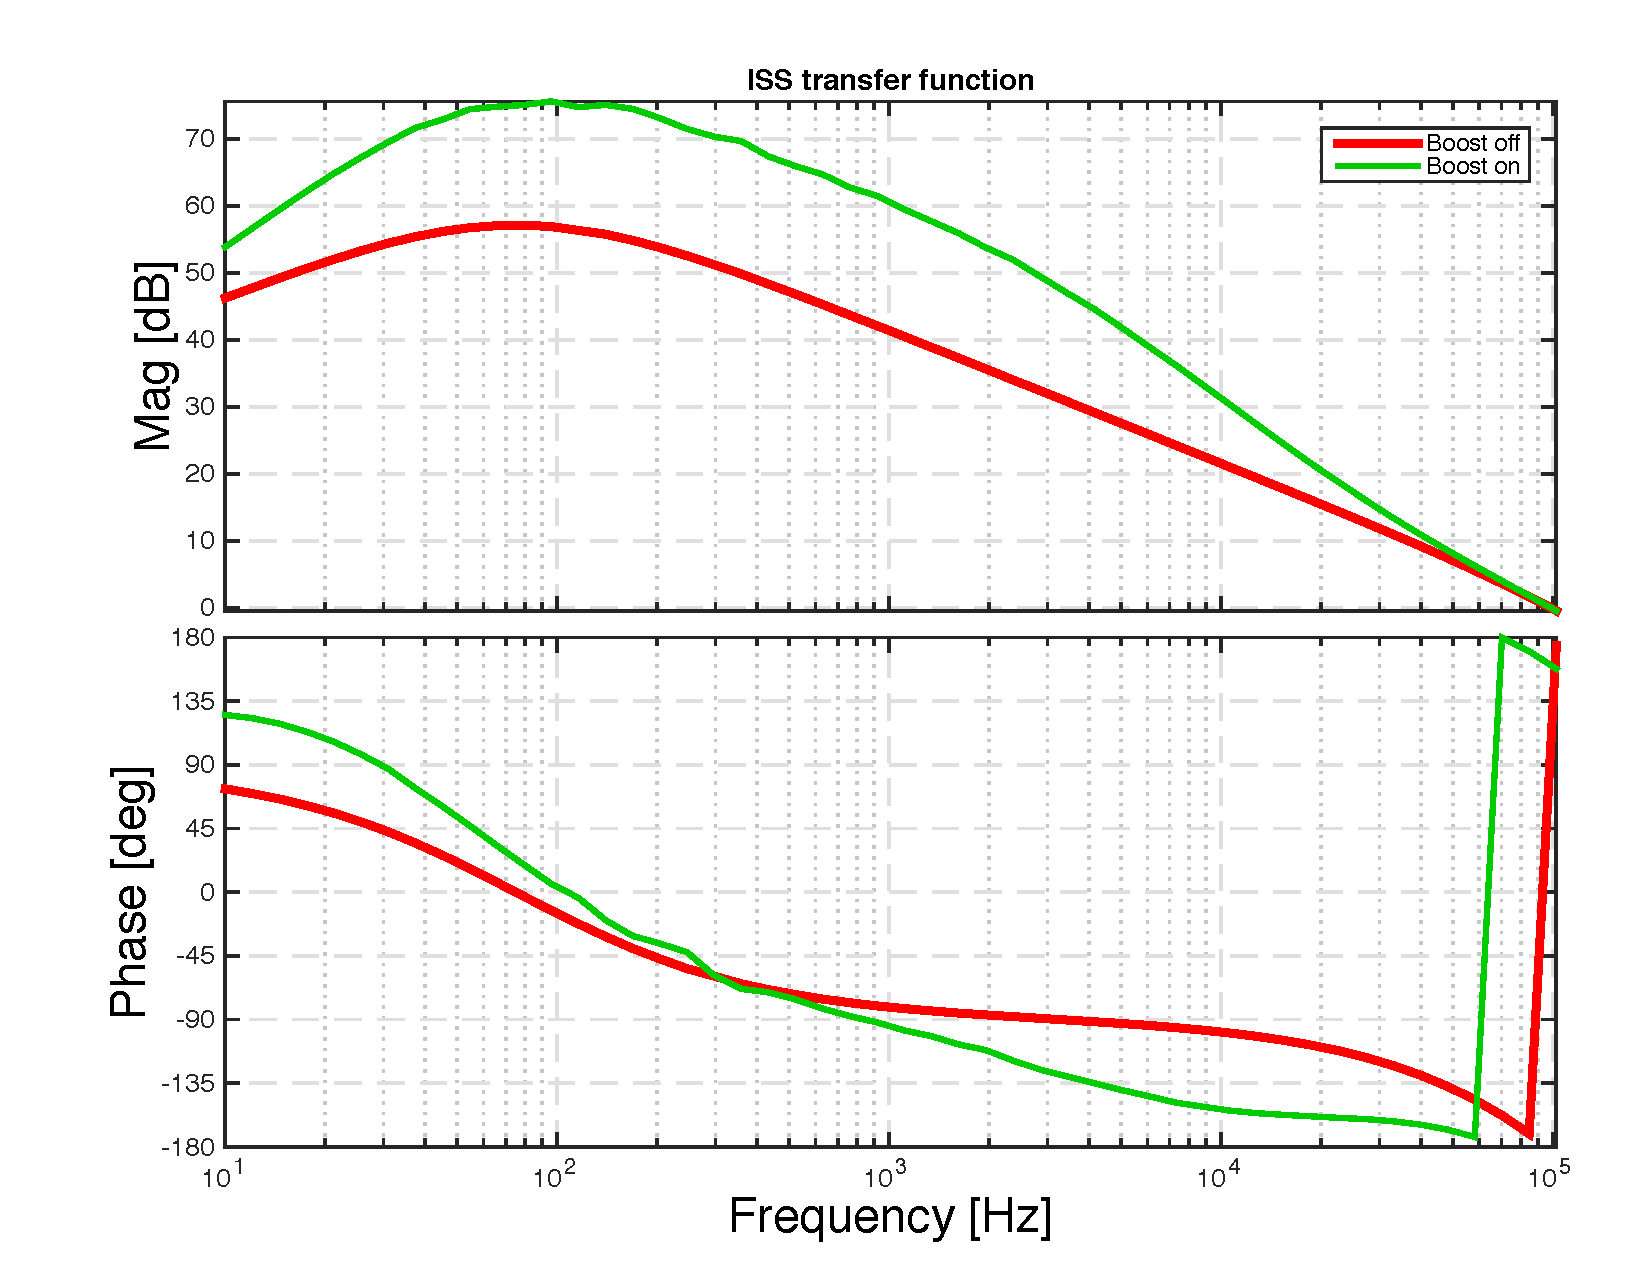
\includegraphics[width=15cm]{./figures/ISStf.pdf}
	\caption[Intensity Stabilization Servo]{
           intensity stabilization servo transfer function.
           This is the open loop transfer function for the ISS.
           The feedback is AC coupled to prevent large DC offsets in the
           actuator.
        }
	\label{fig:isstf}
\end{figure}

\begin{figure}[htbp]
  \centering
  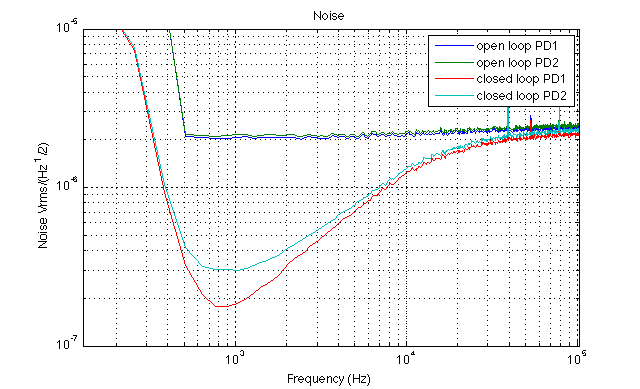
\includegraphics[width=15cm]{./figures/cln.png}
  \caption[ISS Closed Loop Noise]{
    intensity noise with loops closed.
    This plot shows the amount of noise suppression we were able to achieve
    without the \ac{pmc} in place.
    PD1 is the photodiode used for sensing in the active feedback loop.
    PD2 samples the same light but is not in the loop.
    This allows us to measure the actual residual intensity noise, since the
    servo will imprint any sensing noise from PD1 onto the laser intensity.
  }
  \label{fig:isscln}
\end{figure}

\subsection{Sensing}
\todopar{Photo-electric effect, quantum efficiency}

The \ac{pd} works by the photoelectric effect. There is a quantum
efficiency associated with each \ac{pd} which is the amount of light quanta
(photons) which are converted into electrical current.
\begin{align}
q.e. &= \frac{N_{el}}{N_{ph}} \\
     &= \frac{I/e}{P/(\hbar \omega)} \\
     &= \frac{2 \pi \hbar c}{e \lambda} \frac{I}{P} ,
\end{align}
where $e$ is the elementary charge.

This relates the
power of the incident light to the current in the output of the \ac{pd}.
Photodiode quantum efficiency is usually specified in Amps per Watt.
This must naturally be dependent on the wavelength of the light, so they must
also specify a wavelength.

We are limited by noise due to counting statistics (shot noise). We want a high signal
to noise. In this case, the signal that we are concerned about is the
relative fluction in power, and so it is proportional to the DC incident
power on the \ac{pd}. The noise, as a Poissonian process, is proportional
to the square root of the DC power (or the number of photons per second).

The \ac{rin} becomes the photon counting error divided by the total number
of photons.
\begin{align}
\mathrm{RIN} &= \frac{\sqrt{N_{el}}}{N_{el}} \\
     &= \frac{1}{\sqrt{N_{el}}} \\
     &= \frac{1}{\sqrt{q.e. \times N_{ph}}} \\
     &= \sqrt{\frac{\hbar \omega}{q.e. \times P \tau}} \, ,
\end{align}
where $\tau$ is the integration time. This allows us to write the amplitude
spectral density of the shot noise in $\mathrm{RIN} / \sqrt{H\!z}$ as,
\begin{align}
\sqrt{\frac{2 \hbar \omega}{q.e. \times P}} \, ,
\end{align}
where the 2 is due to the choice of one-sided spectra.

% \subsection{Feedback}
% \todopar{Electronics}
% 
% The electronics were designed to reduce intensity noise above about 4 Hz to
% about 1kHz or so. It is in this region where the experiment takes place.

\subsection{Actuation}
\todo{Description of Acousto-Optic Modulator}

Actuation, as mentioned above, is accomplished using an \ac{aom}. The
\ac{aom} is a device which can modulate a laser beam in both frequency
and intensity. It works by using bragg reflections in a crystal with
travelling waves. The interaction between the travelling waves and crystal
lattice divert the beam to different orders of refraction. The power in each
order is dependant on primarily the amplitude of the travelling waves. The
diffraction angle is dependant on the wavelength of the travelling waves.
We take the zero order refraction and modulate on the intensity of the
waves which, in turn, modulated the amount of power diverted into higher order
Bragg refractions.

\section{Frequency Stabilization}
\label{sec:fss}

The \ac{fss} is an active feedback system which stabilizes the already quite
narrow frequency from the laser. The system is composed of a rigid laser cavity
which is used as a reference which we can lock the laser frequency to. The
laser frequency follows the length of the reference cavity up to several kHz.

\subsection{Sensing}

Sensing for the \ac{fss} is accomplished using the method of \ac{pdh}
\cite{Black:2001}.
The signal is essentially the derivative of the reflected power with respect
to frequency of the laser (assuming length is fixed).
This is accomplished by modulating the frequency of the input beam with an
\ac{eom} driven by a 25MHz local oscillator and demodulating the reflected
beam with the same local oscillator.
%This measures the relative amplitude of the reflected light as opposed to the
%amplitude squared (power).
The result is a signal on resonance that is zero and has maximum slope
(see fig.\ref{fig:pdh}).
Exactly the signal we want for a feedback system which keeps the laser on
resonance with the cavity. 

\begin{figure}
\centering
\tikzsetnextfilename{pdhplot}
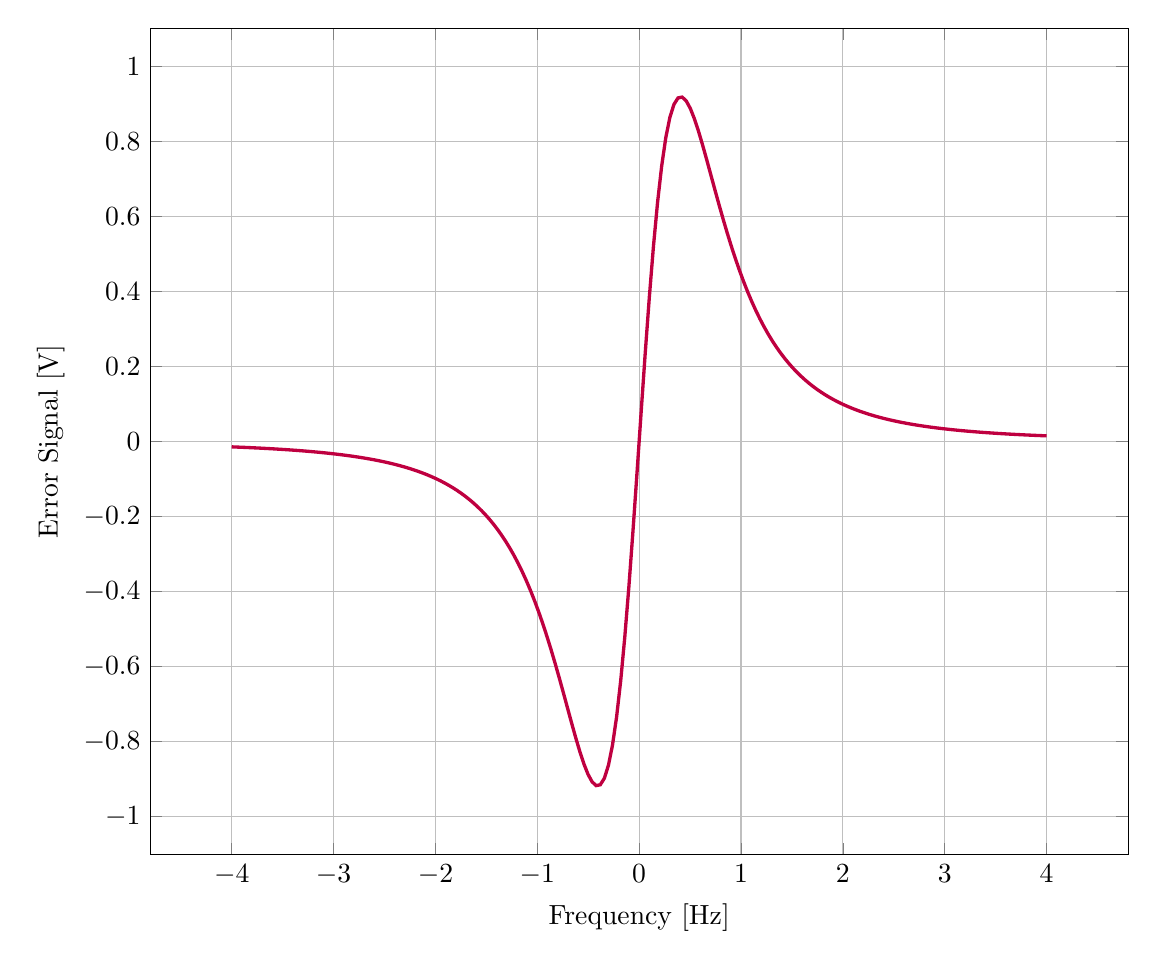
\begin{tikzpicture}
\begin{axis}[
    samples=200,
    grid=both,
    xlabel={Frequency $\left[\mathrm{Hz}\right]$},
    ylabel={Error Signal $\left[\mathrm{V}\right]$}
    ]
%  \addplot[blue,domain=-4:4,very thick] {x*exp(-x*x)};
  \addplot[purple,domain=-4:4,very thick] {x/(x*x+0.5)/(x*x+0.5)};
\end{axis}
\end{tikzpicture}
\caption[PDH Error Signal]{This shows the \ac{pdh} error signal of a simple
  cavity.
  Our lock point must be between the positive and negative cavity poles
  (maximum  and minimum on the y-axis).
  }
\label{fig:pdh}
\end{figure}

\subsubsection{Cavity Assembly}

The reference cavity is a Fabry Perot made from an 8 inch monolithic fused silica
spacer with high reflectivity mirrors glued onto the ends. The reflectivity
of the mirrors yield a finesse of about 7600. Finesse is defined as the ratio
of the \ac{fsr} to the cavity linewidth (\ac{fwhm}).

% One can arrive the
% relationships between FSR, Finesse, mirror reflectivity as follows,
% \begin{align}
% E_{\mathrm{cavity}} =& E_{\mathrm{incident}} \sqrt{1-r_1^2} \left( 1 + r_1 r_2
%     e^{i \omega 2 L /c} + \left(1+r_1 r_2 e^{i \omega 2L/c} \right)^2 + \ldots \right)
%     \\
% =& E_{\mathrm{incident}} \sqrt{1-r_1^2} \left( \frac{1}{1 - r_1 r_2
%     e^{i \omega 2L/c}} \right)
% \end{align}
% Now, we find the reflected field,
% \begin{align}
% E_{\mathrm{reflected}} =& E_{\mathrm{incident}} \left( 1-r_1^2 \right)
%     \left( \frac{r_2 e^{i \omega 2L/c}}{1 - r_1 r_2 e^{i \omega 2L/c}} \right)
%     - r_1 E_{\mathrm{incident}}
% \end{align}

\subsubsection{Cavity Suspension}

The reference cavity is suspended with wires and coil springs from an aluminum
frame. The design of the frame can be seen in figure
\ref{fig:refcav_sus}.
Eddy current dampers were added to damp the resonances. This was done by
attaching vertical aluminum plates to the bottom of the cavity. One was
oriented longitudinally and one laterally.
U-shaped steel channels where attached to the aluminum frame to close the
magnetic field lines of the damping magnets.

\begin{figure}[htbp]
	\centering
		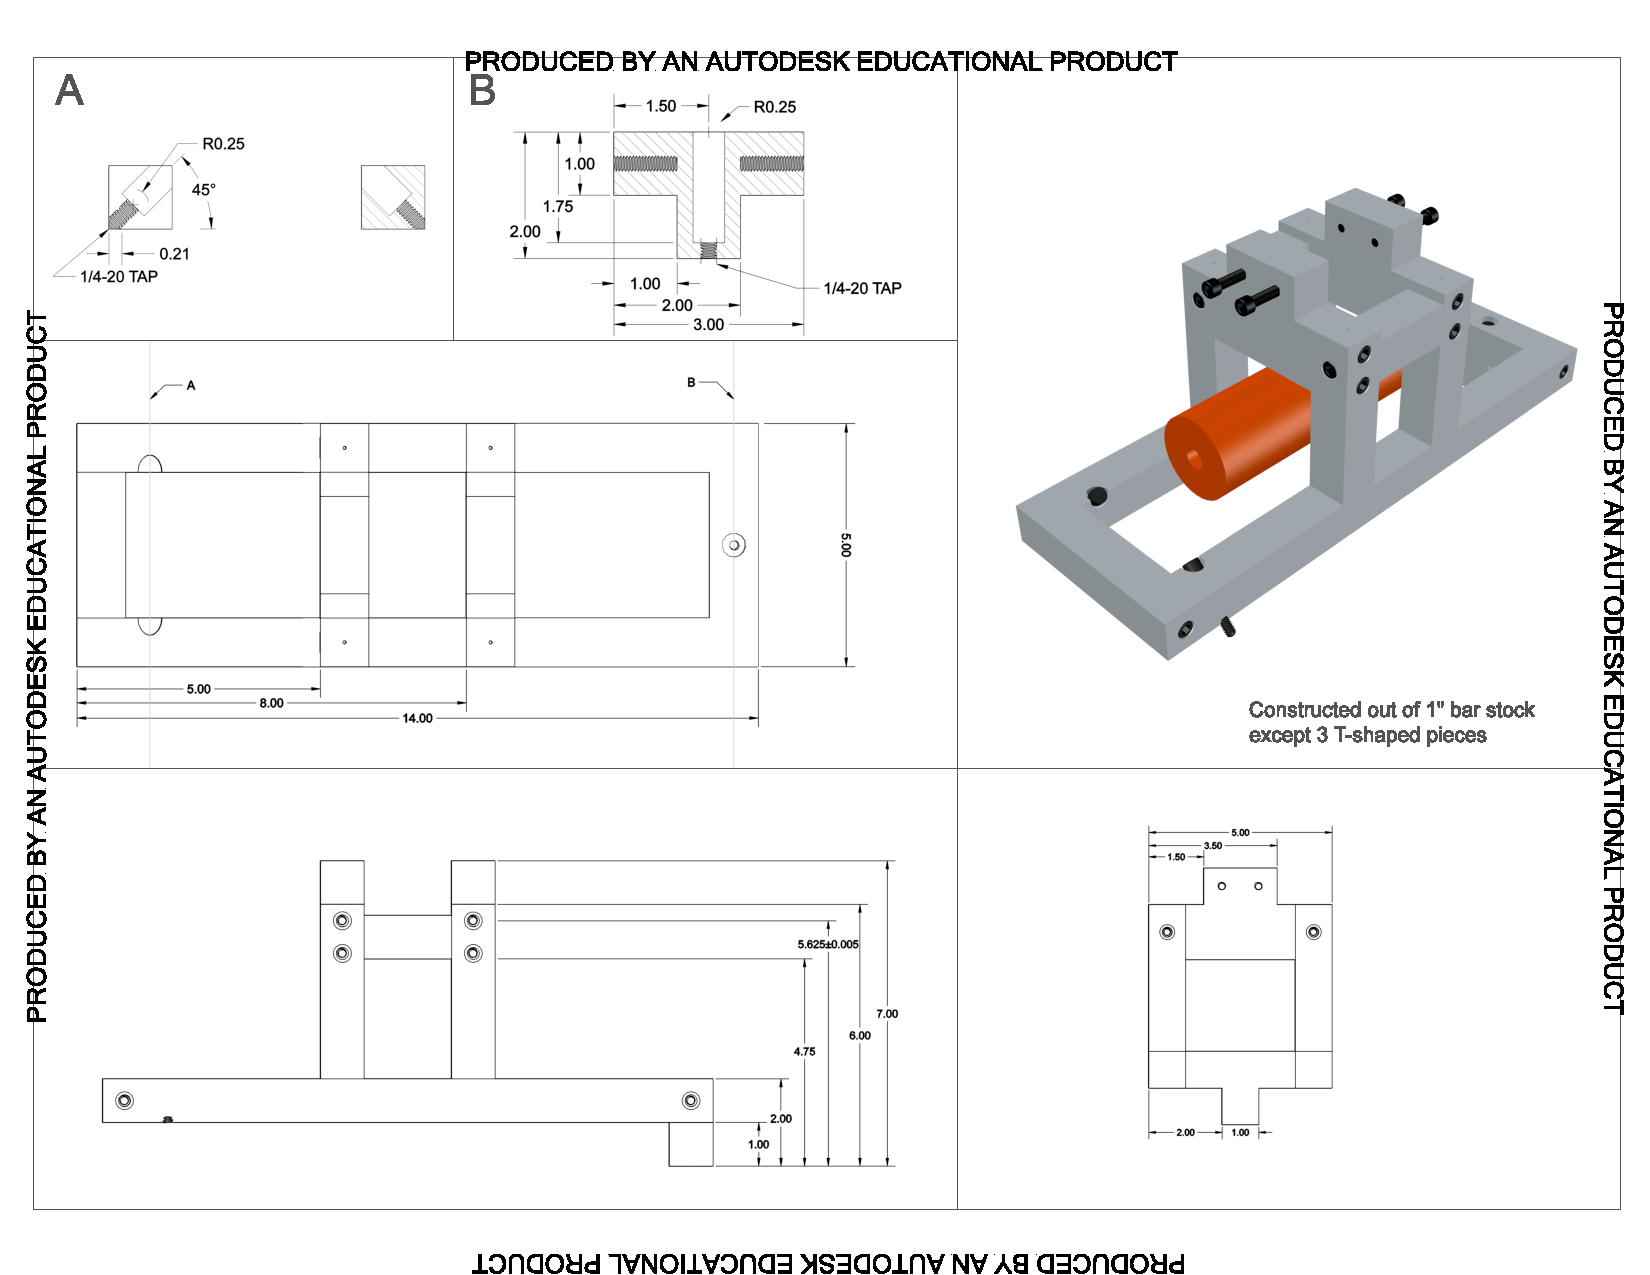
\includegraphics[width=15cm]{./figures/refcavsusdesign.pdf}
	\caption[Reference Cavity Suspension Design]{Design of the reference cavity suspension}
	\label{fig:refcav_sus}
\end{figure}


\subsection{Feedback}
The feedback electronics used for the \ac{fss} are from initial LIGO. The board
provides feedback signal for 2 different actuation paths. The low frequency path
is to the laser cavity length which is split again into two different actuation
paths (thermal control and a piezo electric transducer in the laser head). The
other path is to an \ac{eom} to actuate on the phase of the laser beam.

\subsection{Actuation}

There are three actuators. Low frequency actuation is by a thermal controller in
the laser head which actuates on the the cavity length through thermal expansion.
The mid frequency actuation is by \ac{pzt} which applies a force to change the
cavity length. The high frequency actuation is by phase modulation of the light
after it exits the laser head using an \ac{eom}.

%\todopar{Add a description of the Electro-Optic Modulator}

%\subsubsection{Laser Head Thermal}
%
%\subsubsection{Laser Head Piezo-Electric Transducer}
%\todopar{add description of peizo-electric effect}
%\todopar{describe the effects of the piezo in-loop}

%\subsubsection{Electro Optic Modulator}

%\section{Mode Cleaner}
%\todopar{add description of PMC, reference Willke,98}
%The PMC is a ring cavity of three mirrors.
%see  \cite{Willke:98}


%\subsection{Sensing}

%\subsection{Feedback}

%\subsection{Actuation}
%Actuation on cavity length is done with a piezo-electric transducer on one of
%the mirrors. This transducer converts voltage to cavity length.



\Chapter{Linear Trap Experiment}
\label{ch:lintrapex}

\section{Experimental Layout}
Using the beam from our laser (see \ref{ch:psl}) we split into two orthogonal
polarizations. One beam we need to be at a higher power with positive detuning
(statically stable and dynamically unstable) we call the carrier beam. The
beam with less power and negative detuning we call the subcarrier.

The subcarrier optical path consists of a pair of \ac{aom}s that we use to
detune the subcarrier relative to the carrier beam.
There is also a resonant
\ac{eom} which is used to impart sidebands on the subcarrier beam for \ac{pdh}
locking.
The carrier and subcarrier are then combined using a \ac{pbs} to preserve their
orthogonal polarizations. There is a beamsplitter in the subcarrier path to pick
off the reflected light from the cavity which is used to generate the \ac{pdh}
signal. There are additional $\lambda/2$ and $\lambda/4$ waveplates at various
points in the path for polarization optimization.

\subsection{Subcarrier Servo}
Because of our short cavity length we have a large \ac{fsr} in frequency of
about 2.14GHz.
This produces a technical problem in attempting to set the
subcarrier on the next resonance, one \ac{fsr} away.
\ac{aom}s are limited in the range of frequencies they can operate in.
The minimum is higher than the linewidth for our cavity.
The maximum is less than \ac{fsr}.

The solution for us was to set the subcarrier on the same resonance fringe
using two \ac{aom}s, each one shifting the frequency by about 80MHz in
opposite directions.
One is driven by a crystal oscillator.
The other is driven by a tunable oscillator, a \ac{vco}, which gives us the
knob to detune the subcarrier.

We produce a beat signal between the two oscillators and we lock the beat
signal to a function generator operating in the range of frequencies we are
need to detune the subcarrier with. So, now we can set directly, the carrier
to subcarrier offset frequency using the knob on the function generator.
This setup essentially eliminates frequency noise due to the crystal
oscillator, which is quite low to begin with, since we are subtracting the
same, coherent, frequency noise with the second \ac{aom}.
And the frequency noise due to the function generator is lower due to the
fact that we are using a lower frequency tunable oscillator.
Tunable oscillators generally have a frequency noise that is relative to the
set frequency.

\section{Features of Experiment}
\subsection{High Finesse}
We need a high finesse cavity to give us the power buildup in the cavity that
we need for a decent resonant frequency to get beyond some environmental noise.
Ignoring any damping effects a fairly straight-forward calculation gives the
resonant frequency we can achieve for a given finesse and input power. For a
high finesse, it can be shown that the maximum spring constant for a given
power is approximately,
\begin{align}
k &= \frac{18 F^2}{\sqrt{12} \pi \lambda c} P
\end{align}
which gives a maximum resonant frequency of,
\begin{align}
f_0 &= \frac{F}{2 \pi} \sqrt{\frac{18 P}{\sqrt{12} \pi \lambda m c }} \\
&\approx 3.8kHz
\end{align}

\subsection{Short Cavity}
The short cavity gives us a reduction in the frequency noise contribution
to the noise budget. This reduction scales as the cavity length. This also
affects the free spectral range, however, and with our finesse, the cavity
pole is about 140kHz. 

\subsection{High Spring Frequency}

\begin{figure}[htbp]
\tikzsetnextfilename{roomlayout}
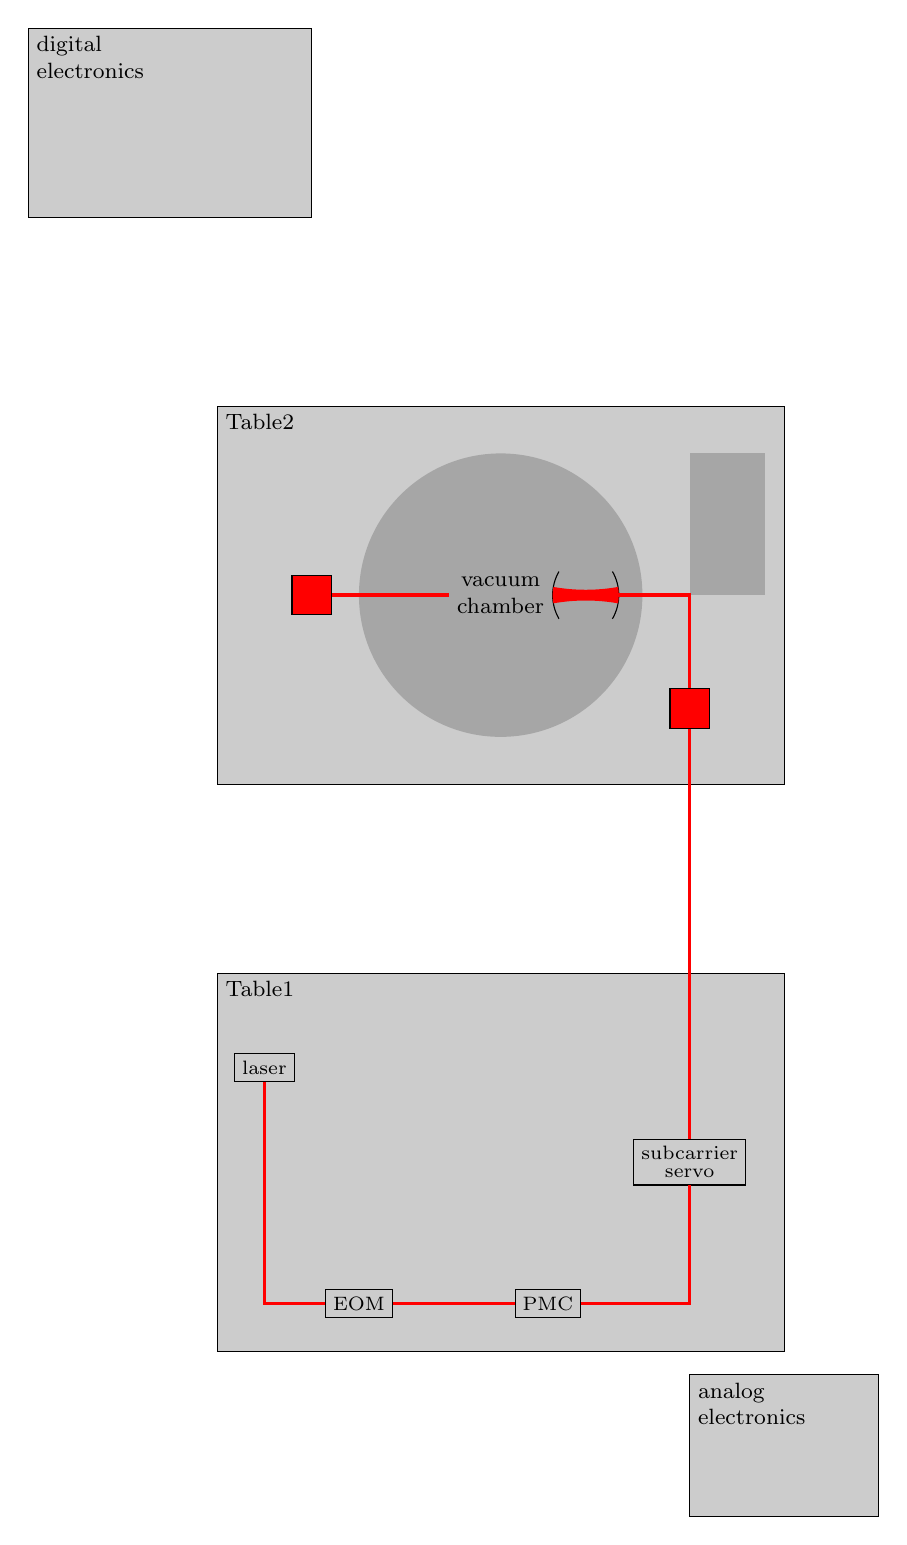
\begin{tikzpicture}[scale=1.2]
    \begin{footnotesize}
    \renewcommand{\baselinestretch}{1}
    \filldraw[fill=white!60!gray,draw=black] (8,2) rectangle (2,6)
        node[black,align=left,anchor=north west] {Table1};
    \filldraw[fill=white!60!gray,draw=black] (8,8) rectangle (2,12)
        node[black,align=left,anchor=north west] {Table2};
    \filldraw[fill=white!60!gray,draw=black] (3,14) rectangle (0,16)
        node[black,align=left,anchor=north west] { digital \\ electronics };
    \filldraw[fill=white!60!gray,draw=black] (9,0.25) rectangle (7,1.75)
        node[black,align=left,anchor=north west] { analog \\ electronics };
    \fill[white!30!gray] (5,10) circle (1.5)
        node[black,align=center] (v0) { vacuum \\ chamber };
    \fill[white!30!gray] (7,10) rectangle (7.8,11.5);
    \end{footnotesize}
    \begin{scriptsize}
    \renewcommand{\baselinestretch}{0.8}
    \draw (2.5,5) node(laser) [draw] {laser}
        (3.5,2.5) node(eom) [draw] {EOM}
        (5.5,2.5) node(pmc) [draw] {PMC}
        (7,4) node[align=center](scs) [draw] {subcarrier \\ servo}
        (7,8.8) node[align=center,fill=red,minimum height=0.5cm,minimum width=0.5cm](peris) [draw] {}
        (3,10) node[align=center,fill=red,minimum height=0.5cm,minimum width=0.5cm](peris2) [draw] {}
        (7,10) node(io) {};
    \end{scriptsize}
    \draw (5.75,10) ++(-30:0.5cm) arc (-30:30:0.5);
    \draw (5.55,10) arc (180:150:0.5)
        arc (150:210:0.5);
    \fill[red] (5.75,10) ++(-10:0.5cm) arc (-10:10:0.5)
        arc (280:260:1.971825337) arc (170:190:0.5) arc (100:80:1.971825337);
    \draw[red,very thick] (laser.south) |- (eom.west);
    \draw[red,very thick] (eom.east) |- (pmc.west);
    \draw[red,very thick] (pmc.east) -| (scs.south);
    \draw[red,very thick] (scs.north) |- (peris.south);
    \draw[red,very thick] (peris.north) |- (v0.east);
    \draw[red,very thick] (v0.west) -| (peris2.east);
\end{tikzpicture}
\caption[Room Layout]{This depicts the basic layout of how the experiment
    is situated in the lab. The red boxes on table 2 are periscopes necessary
    for getting the laser to the height of the trap cavity, and on the ouput
    side for getting back to the table height for the output optics.}
\label{fig:roomlayout}
\end{figure}

\begin{figure}
\tikzsetnextfilename{traploops}
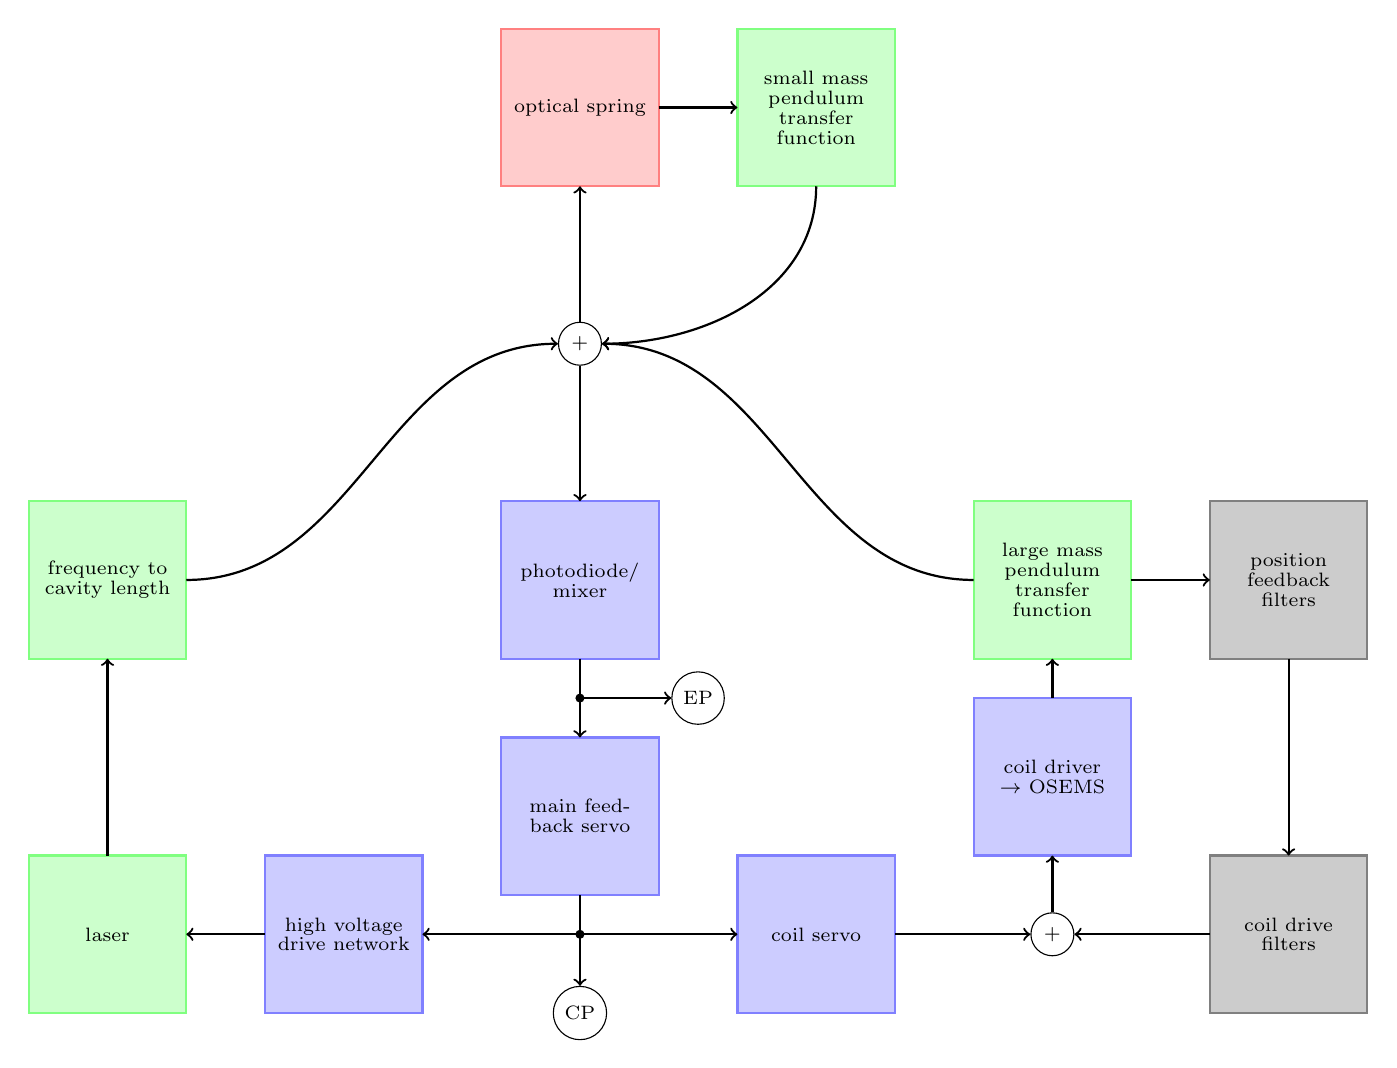
\begin{tikzpicture}
  [analog/.style={rectangle,draw=blue!50,fill=blue!20,thick,align=center,
                  outer sep=0,minimum size=2cm,text width=1.8cm},
   digital/.style={rectangle,draw=black!50,fill=black!20,thick,align=center,
                   outer sep=0,minimum size=2cm,text width=1.8cm},
   physical/.style={rectangle,draw=green!50,fill=green!20,thick,align=center,
                    outer sep=0,minimum size=2cm,text width=1.8cm},
   optical/.style={rectangle,draw=red!50,fill=red!20,thick,align=center,
                   outer sep=0,minimum size=2cm,text width=1.8cm}]
  \renewcommand{\baselinestretch}{0.9}
  \begin{scriptsize}
  \node[circle,draw=black] (sum) at (0,0) {+};
  \node[circle,draw=black] (sumcoil) at (6,-7.5) {+};
  \node[circle,draw,fill=black,minimum size=0.1cm,inner sep=0,outer sep=0] (intersection1) at (0,-4.5) {};
  \node[circle,draw,fill=black,minimum size=0.1cm,inner sep=0,outer sep=0] (intersection2) at (0,-7.5) {};
  \node[analog] (X) at (0,-3) {photodiode/ mixer};
  \node[analog] (F) at (0,-6) {main feedback servo};
  \node[analog] (T) at (3,-7.5) {coil servo};
  \node[analog] (C) at (6,-5.5) {coil driver $\rightarrow$ OSEMS};
  \node[physical] (P) at (6,-3) {large mass pendulum transfer function};
%  \node[analog] (A) [below=of F] {attenutation for digital system input};
  \node[digital] (D) at (9,-3) {position feedback filters};
  \node[digital] (E) at (9,-7.5) {coil drive filters};
  \node[analog] (H) at (-3,-7.5) {high voltage drive network};
  \node[physical] (L) at (-6,-7.5) {laser};
  \node[physical] (M) at (-6,-3) {frequency to cavity length};
  \node[optical] (O) at (0,3) {optical spring};
  \node[physical] (S) at (3,3) {small mass pendulum transfer function};
  \node[circle,draw=black] (ep) at (1.5,-4.5) {EP};
  \node[circle,draw=black] (cp) at (0,-8.5) {CP};
  \draw[thick,->] (sum) to (X);
  \draw[thick] (X) to (intersection1);
  \draw[thick,->] (intersection1) to (F);
  \draw[thick] (F) to (intersection2);
  \draw[thick,->] (intersection2) to (T);
  \draw[thick,->] (T) to (sumcoil);
  \draw[thick,->] (sumcoil) to (C);
%  \draw[thick,->] (F) to (A);
  \draw[thick,->] (intersection2) to (H);
  \draw[thick,->] (intersection2) to (cp);
  \draw[thick,->] (H) to (L);
  \draw[thick,->] (L) to (M);
%  \draw[thick,->] (A) to [out=0,in=270] (E);
  \draw[thick,->] (P) to (D);
  \draw[thick,->] (D) to (E);
  \draw[thick,->] (C) to (P);
  \draw[thick,->] (E) to (sumcoil);
  \draw[thick,->] (P) to [out=180,in=0] (sum);
  \draw[thick,->] (sum) to (O);
  \draw[thick,->] (O) to (S);
  \draw[thick,->] (M) to [out=0,in=180] (sum);
  \draw[thick,->] (S) to [out=270,in=0] (sum);
  \draw[thick,->] (intersection1) to (ep);
  \end{scriptsize}
\end{tikzpicture}
\caption[Trapping Loops]{This chart depicts the feedback scheme used for
         locking the trapping cavity and observing the spring behavior.}
\end{figure}

\begin{figure}
\tikzsetnextfilename{scservo}
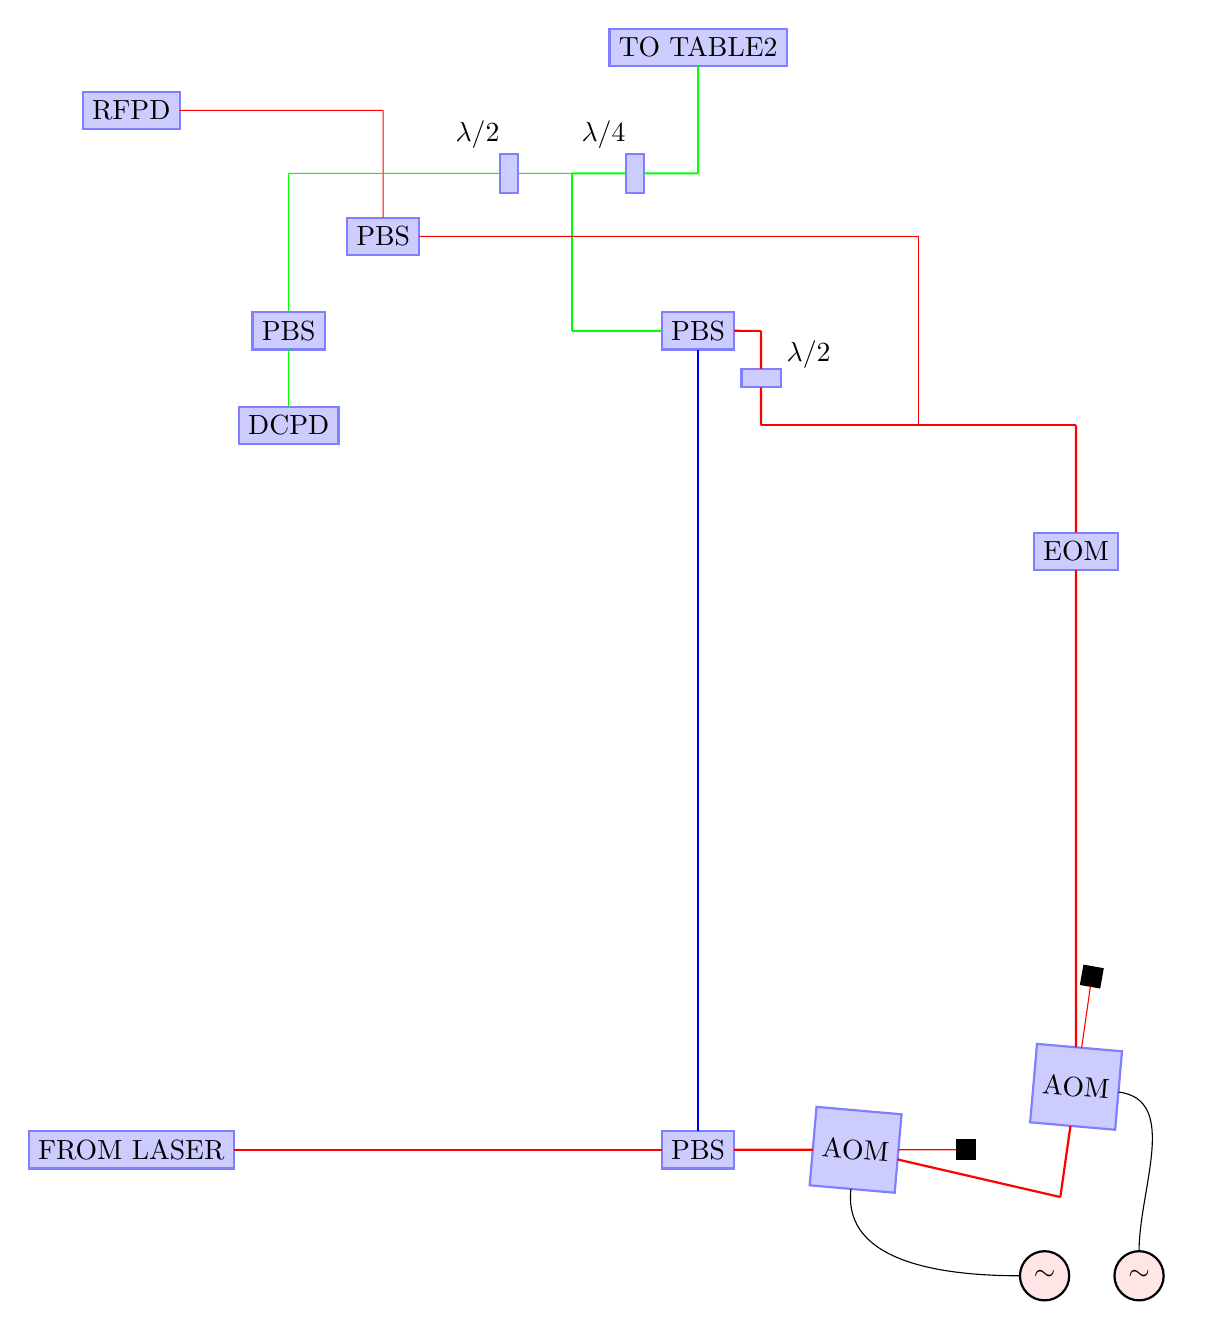
\begin{tikzpicture}
  [scale=0.4,
%  mirror/.style={rectangle,draw=blue!50,fill=blue!20,thick,align=center,
%                  outer sep=0},
  mirror/.style={rectangle,outer sep=0,minimum size=0cm},
  eom/.style={rectangle,draw=blue!50,fill=blue!20,thick,align=center,
                  outer sep=0},
  aom/.style={rectangle,draw=blue!50,fill=blue!20,thick,align=center,
                  outer sep=0,minimum size=1cm},
  pbs/.style={rectangle,draw=blue!50,fill=blue!20,thick,align=center,
                  outer sep=0},
  rfpd/.style={rectangle,draw=blue!50,fill=blue!20,thick,align=center,
                  outer sep=0},
  dcpd/.style={rectangle,draw=blue!50,fill=blue!20,thick,align=center,
                  outer sep=0},
  bblock/.style={rectangle,draw=black,fill=black,thick,align=center,
                  outer sep=0},
  lambdaplate/.style={rectangle,draw=blue!50,fill=blue!20,thick,align=center,
                  outer sep=0},
  beamenter/.style={rectangle,draw=blue!50,fill=blue!20,thick,align=center,
                  outer sep=0},
  beamexit/.style={rectangle,draw=blue!50,fill=blue!20,thick,align=center,
                  outer sep=0},
  osc/.style={circle,draw=black,fill=red!10,thick,align=center,
                  outer sep=0}
                  ]
%  \renewcommand{\baselinestretch}{0.9}

%  \begin{scriptsize}
  \node[beamenter] (laserin) at (-32,7) {FROM LASER};
  \node[beamexit] (laserout) at (-14,42) {TO TABLE2};
  \node[pbs] (pbs1) at (-14,7) {PBS};
  \node[aom,rotate=-5] (aom1) at (-9,7) {AOM};
  \node[bblock] (bb1) at (-5.5,7) {};
  \coordinate (m1) at (-2.5,5.5) {};
  \node[aom,rotate=-5] (aom2) at (-2,9) {AOM};
  \node[bblock,rotate=-10] (bb2) at (-1.5,12.5) {};
  \node[eom] (eom1) at (-2,26) {EOM};
  \coordinate (m2) at (-2,30) {};
  \coordinate (m3) at (-7,30) {};
  \coordinate (m4) at (-12,30) {};
  \coordinate (m5) at (-12,33) {};
  \node[pbs] (pbs2) at (-14,33) {PBS};
  \coordinate (m6) at (-18,33) {};
  \coordinate (m7) at (-18,38) {};
  \coordinate (m8) at (-14,38) {};
  \coordinate (m9) at (-7,36) {};
  \node[pbs] (pbs3) at (-24,36) {PBS};
  \coordinate (m10) at (-24,40) {};
  \node[rfpd] (rfpd1) at (-32,40) {RFPD};
  \coordinate (mrefl21) at (-27,38) {};
  \node[pbs] (pbsrefl2) at (-27,33) {PBS};
  \node[dcpd] (dcpd1) at (-27,30) {DCPD};
  \node[lambdaplate,minimum height=0.5cm] (lambda1) at (-16,38) {};
  \node[anchor=south east] (lambdat1) at (-16,38.5) {$\lambda/4$};
  \node[lambdaplate,minimum height=0.5cm] (lambda2) at (-20,38) {};
  \node[anchor=south east] (lambdat2) at (-20,38.5) {$\lambda/2$};
  \node[lambdaplate,minimum width=0.5cm] (lambda3) at (-12,31.5) {};
  \node[anchor=south west] (lambdat3) at (-11.5,31.5) {$\lambda/2$};
  \node[osc] (oscx) at (-3,3) {$\sim$};
  \node[osc] (oscv) at (0,3) {$\sim$};
  \draw[thick,red] (pbs1) to (aom1);
  \draw[thick,red] (aom1) to (m1);
  \draw[red] (aom1) to (bb1);
  \draw[thick,red] (m1) to (aom2);
  \draw[thick,red] (aom2) to (eom1);
  \draw[red] (aom2) to (bb2);
  \draw[thick,red] (eom1) to (m2);
  \draw[thick,red] (m2) to (m3);
  \draw[thick,red] (m3) to (m4);
  \draw[thick,red] (m4) to (lambda3);
  \draw[thick,red] (lambda3) to (m5);
  \draw[thick,red] (m5) to (pbs2);
  \draw[thick,green] (pbs2) to (m6);
  \draw[thick,green] (m6) to (m7);
  \draw[thick,green] (m7) to (lambda1);
  \draw[thick,green] (lambda1) to (m8);
  \draw[red] (m3) to (m9);
  \draw[red] (m9) to (pbs3);
  \draw[red] (pbs3) to (m10);
  \draw[red] (m10) to (rfpd1);
  \draw[thick,blue] (pbs1) to (pbs2);
  \draw[thick,red] (laserin) to (pbs1);
  \draw[thick,green] (m8) to (laserout);
  \draw[green] (m7) to (lambda2);
  \draw[green] (lambda2) to (mrefl21);
  \draw[green] (mrefl21) to (pbsrefl2);
  \draw[green] (pbsrefl2) to (dcpd1);
  \draw[black] (aom1) to [in=180,out=265] (oscx);
  \draw[black] (aom2) to [in=90,out=355] (oscv);
%  \end{scriptsize}
\end{tikzpicture}
\caption[Subcarrier Servo]{This is a schematic of the optical path for the
         subcarrier servo on Table 1.}
\end{figure}


%\tikzsetnextfilename{gaussian3d}
%\begin{tikzpicture}
%\begin{axis}[
%        view={0}{45},
%        hide axis,
%        xlabel=$x$,ylabel=$y$,
%        mesh/interior colormap name=hot,
%        colormap/blackwhite, 
% ]
%  \addplot3[domain=-1.5:1.5,surf]
%        {exp(-x^2-y^2)};
%\end{axis}
%\end{tikzpicture}

\section{High-Q Payload Suspension}

In designing the suspension for the small mirror we went through the thermal
noise analysis to determine the best approach. We wanted to suspend the small
mirror using thin glass fibers with a low tension for isolating the mass from
vibrations in the next mass up in the chain.

The initial thermal noise analysis was for the glue used to mount the glass
fibers to the small mirror. This analysis is described in detail in the
noise chapter. We designed the glue joints of the suspension to minimize
thermal noise based on the analysis. The result of the analysis was to have a
small mass at the glue end of the fiber with a center of gravity close to the
glue surface.

\subsection{Monolithic Welding}

We began by gaining experience with welding fibers. In doing so, we decided it
should not be too difficult to weld the fibers directly to the small mirror.
This actually proved to be more difficult than anticipated.
The first attempt at welding a mirror damaged the coating quite visibly even
though we were careful to shield the coating surface by clamping the mirror
with quartz tubes.

After making several improvements to the welding stand, we welded a mirror
with no visible damage to the coating, however once installed, we found the
finesse to be too low.
The mirror was welded, suspended, and placed in vacuum system
for assembly of the cavity.
After careful alignment we found the finesse to be about 700, much lower than
desired.
Since this was the cavity output mirror that was damaged, it dramatically
affected the performance of the experiment.
The power buildup in the cavity is dependent on the
individual cavity mirror reflectivities.

\subsection{Glued Fiber Attachements}

The final suspension design for this experiment used small cone-shaped glass
nubs at the glue end of the fibers. This could be constructed monolithicaly
by cold welding\footnote{a process where the substrate is not heated to the
point where the materials flow together} the tip of a glass rod to a small
mirror blank\footnote{or a mirror with a previously damaged coating...} to
create a small nub from which the fiber is pulled. This is all done in one
continuous motion where the torch is applied to the edge of the mirror to
gently heat the point of attachement, then the rod with a sharp point is placed
into the flame to melt the tip and cold weld to the edge of the mirror. The
flame is then directed at the tip of the rod slightly back from the weld to
soften the fiber pull spot. When the spot is sufficiently heated, the fiber
is pulled away sharply while dropping the flame away from the fiber. What
remains is a rod attached to a small conical shaped nub monolithically through
a very thin, high Q fiber. Now the cold weld allows us to separate this
monolithic fiber assembly because the bond strength is much less than the yield
strength of the fiber. We then glue this monolithic fiber assembly using the
epoxy to the side of the mirror with undamaged coatings. This technique allows
us to preserve a very high Q (~$5x10^5$) while avoiding damage to the coating.

\subsection{Double Pendulum}
The output mirror is suspended by glass fibers inside a ring of steel which is
three inches in diameter. The steel ring is the \ac{sos} controlled mass.
Since the mass of the ring is considerably greater than the mass of the small
mirror, the transfer function for force to position on the small mirror can be
approximated by simply the small mirror mass and resonant frequency.
For the complete solution, the equations of motion that need to be solved for
one dimension are,

\begin{figure}
\tikzsetnextfilename{smallmass}
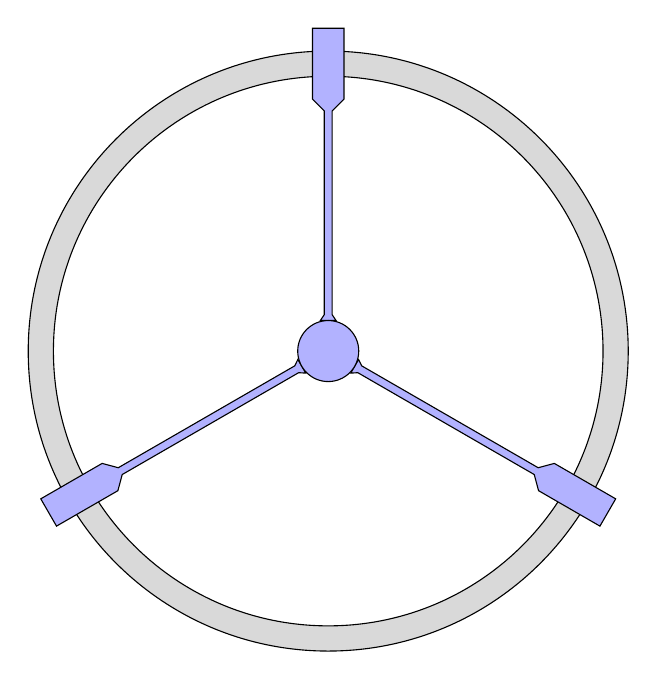
\begin{tikzpicture}
  \begin{scope}[even odd rule]
    \fill[fill=gray!30!white] (0,0) circle(3.49cm) (0,0) circle(3.81cm);
  \end{scope}
  \draw (0,0) circle(3.49);
  \draw (0,0) circle(3.81);
  \filldraw[fill=blue!30!white]
    (0.2,3.2) -- (0.2,4.1) -- (-0.2,4.1) -- (-0.2,3.2) --
    (-0.05,3.05) -- (-0.05,0.4625) -- (-0.1,0.3875) --
    (0.1,0.3875) -- (0.05,0.4625) --
    (0.05,3.05) -- cycle;
  \filldraw[fill=blue!30!white,rotate=120]
    (0.2,3.2) -- (0.2,4.1) -- (-0.2,4.1) -- (-0.2,3.2) --
    (-0.05,3.05) -- (-0.05,0.4625) -- (-0.1,0.3875) --
    (0.1,0.3875) -- (0.05,0.4625) --
    (0.05,3.05) -- cycle;
  \filldraw[fill=blue!30!white,rotate=240]
    (0.2,3.2) -- (0.2,4.1) -- (-0.2,4.1) -- (-0.2,3.2) --
    (-0.05,3.05) -- (-0.05,0.4625) -- (-0.1,0.3875) --
    (0.1,0.3875) -- (0.05,0.4625) --
    (0.05,3.05) -- cycle;
  \filldraw[fill=blue!30!white] (0,0) circle(0.3875);
\end{tikzpicture}
\caption[Small Mirror Suspension]{The small mirror suspension intermediate
         mass (gray) is a 3 inch diameter steel ring about 1/4" thick and 1"
         deep. The small mirror itself is a 7.75mm diameter fused silica
         substrate with a 5cm radius of curvature. The suspension fibers are
         monolithic to a small conical nub which is glued to the outside edge
         of the mirror.}
\end{figure}


\begin{figure}
\tikzsetnextfilename{doublesus}
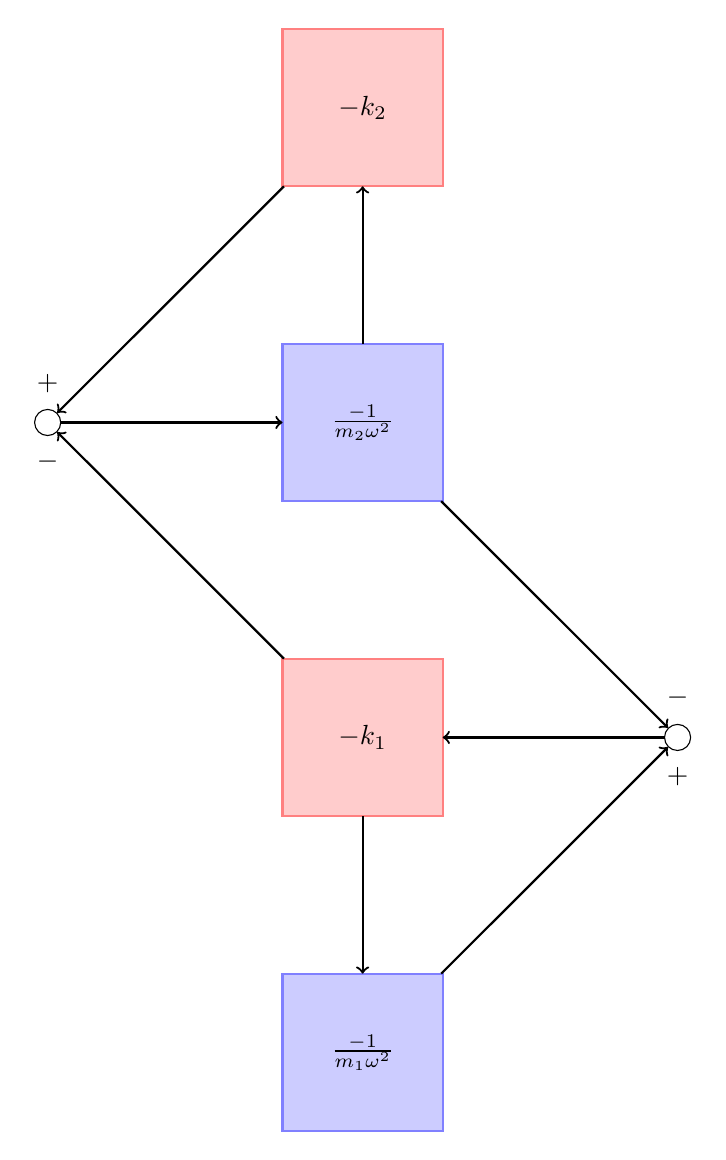
\begin{tikzpicture}
  [mass/.style={rectangle,draw=blue!50,fill=blue!20,thick,align=center,
                  outer sep=0,minimum size=2cm,text width=1.8cm},
   digital/.style={rectangle,draw=black!50,fill=black!20,thick,align=center,
                   outer sep=0,minimum size=2cm,text width=1.8cm},
   physical/.style={rectangle,draw=green!50,fill=green!20,thick,align=center,
                    outer sep=0,minimum size=2cm,text width=1.8cm},
   spring/.style={rectangle,draw=red!50,fill=red!20,thick,align=center,
                   outer sep=0,minimum size=2cm,text width=1.8cm}]
%  \renewcommand{\baselinestretch}{0.9}
%  \begin{small}
  \node[spring] (spring2) at (0,0) {$-k_2$};
  \node[mass] (mass2) at (0,-4) {$\frac{-1}{m_2\omega^2}$};
  \node[spring] (spring1) at (0,-8) {$-k_1$};
  \node[mass] (mass1) at (0,-12) {$\frac{-1}{m_1\omega^2}$};
  \node[circle,draw=black] (sum2) at (-4,-4) {};
  \node (plus2) at (-4,-3.5) {$+$};
  \node (minus2) at (-4,-4.5) {$-$};
  \node[circle,draw=black] (sum1) at (4,-8) {};
  \node (plus1) at (4,-8.5) {$+$};
  \node (minus1)  at (4,-7.5) {$-$};
  \draw[thick,->] (spring2) to (sum2);
  \draw[thick,->] (sum2) to (mass2);
  \draw[thick,->] (mass2) to (spring2);
  \draw[thick,->] (mass2) to (sum1);
  \draw[thick,->] (sum1) to (spring1);
  \draw[thick,->] (spring1) to (sum2);
  \draw[thick,->] (spring1) to (mass1);
  \draw[thick,->] (mass1) to (sum1);
%\end{small}
\end{tikzpicture}
\caption[Double Pendulum Feedback Representation]{This diagram represents the
         double pendulum feedback loops from which one can calculate the
         response of the system.}
\end{figure}

\section{Locking Challenges}

\subsection{Optical Lever}
We found the small mirror resonances to be strong enough to prevent locking the
trapping cavity. Our solution to this was to employ an optical lever, where a
laser is reflected off the back of the small mirror and onto a quadrant
photodiode. The photodiode outputs a signal corresponding to the pitch and yaw
of the small mirror. If you aren't careful with the position of lenses, there
will be a coupling of the small mirror position to the photodiode signals.
We took advantage of our carelessness and used the coupled position signal
to feedback through resonant gain filters in the digital system and applied to
the OSEM drives of the SOS.

\section{Actuation Range}
Due to seismic noise we needed a fairly wide actuation range at low frequencies.
The maximum range of the laser PZT is plus or minus 160MHz. This corresponds to
about 42nm. We needed another actuation path to extend the range at low
frequencies. For this we use the magnetic force from the OSEM coils.
Additionally, due to the high finesse, we needed a fairly high bandwidth for
the feedback loop. The high voltage amplifier for the laser PZT itself has a
bandwidth limit, so we needed a high-frequency bypass which passively adds the
HV output to the HV input.

\section{Sub-Carrier Servo}
As mentioned above, we needed a way of shifting the frequency of the subcarrier
beam in relation to the carrier by $\mathcal{O}\, 100\, kH\!z$.
We do this using \ac{aom}s by first shifting in one direction by $80\,MH\!z$,
then shifting the opposite direction by $80\,MH\!z + \mathrm{offset}$.
The $80\,MH\!z$ frequency source is a crystal oscillator. The variable
frequency source is a \ac{vco} which uses the output of a feedack servo to
modulate the frequency. The sensor for this feedback is the demodulated beat
signal of the output of the two \ac{aom} frequency sources. The demodulation
is done by mixing the beat signal with the output of a function generator which
is set to the desired offset frequency.

\begin{figure}
\centering
\tikzsetnextfilename{scsfeedback}
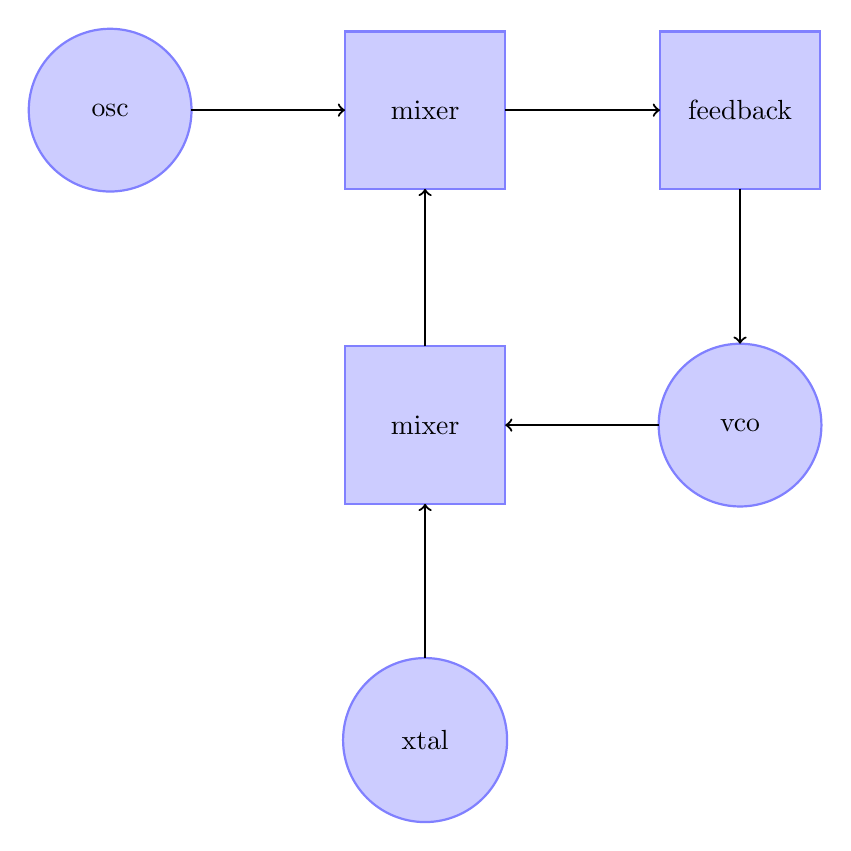
\begin{tikzpicture}
  [block/.style={rectangle,draw=blue!50,fill=blue!20,thick,align=center,
                  outer sep=0,minimum size=2cm,text width=1.8cm},
   oscillator/.style={circle,draw=blue!50,fill=blue!20,thick,align=center,
                  outer sep=0,minimum size=2cm,text width=1.8cm},
   digital/.style={rectangle,draw=black!50,fill=black!20,thick,align=center,
                   outer sep=0,minimum size=2cm,text width=1.8cm},
   physical/.style={rectangle,draw=green!50,fill=green!20,thick,align=center,
                    outer sep=0,minimum size=2cm,text width=1.8cm},
   spring/.style={rectangle,draw=red!50,fill=red!20,thick,align=center,
                   outer sep=0,minimum size=2cm,text width=1.8cm}]
%  \renewcommand{\baselinestretch}{0.9}
%  \begin{small}
  \node[block] (servo) at (0,0) {feedback};
  \node[block] (mixer2) at (-4,0) {mixer};
  \node[block] (mixer1) at (-4,-4) {mixer};
  \node[oscillator] (osc1) at (0,-4) {vco};
  \node[oscillator] (osc2) at (-4,-8) {xtal};
  \node[oscillator] (osc3) at (-8,0) {osc};
  \draw[thick,->] (servo) to (osc1);
  \draw[thick,->] (osc2) to (mixer1);
  \draw[thick,->] (osc3) to (mixer2);
  \draw[thick,->] (mixer1) to (mixer2);
  \draw[thick,->] (osc1) to (mixer1);
  \draw[thick,->] (mixer2) to (servo);
%\end{small}
\end{tikzpicture}
\caption[Subcarrier Servo Electronics]{This diagram represents the
         subcarrier servo feedback.}
\end{figure}

\subsection{Noise Requirements}

\section{Relative Power Tuning}

\section{Differential Power Fluctuations}

\section{Procedures}

\subsection{Measure the optical losses up to the cavity}

\subsection{Calibration of carrier and subcarrier photodiodes}
We will calibrate the photodiodes while the cavity is not locked, knowing the incident beam power and the round trip losses.

\begin{itemize}
    \item Block carrier light in Mach-Zehnder path.
    \item Turn the reflection monitor beam half-wave plate to minimize subcarrier light on the photodiode.
    \item Block the reflection monitor beam to measure dark voltage at DCPD ($A$).
    \item Unblock the reflection monitor beam and measure voltage at DCPD ($B$).
    \item Unblock the carrier light and measure again ($C$)
    \item Block subcarrier light and measure the carrier power using power meter after last steering mirror on table 1 ($D$).
    \item Using the measured optical loss to the cavity ($L$) compute the mW/mV calibration:
    \begin{itemize}
        \item $\frac{D\cdot L}{C - B}$
    \end{itemize}
\end{itemize}

\section{Mode Matching}
We want to know how much power couples into the cavity from a
perfectly gaussian beam of the wrong size and location. We start with
the equations for the Hermite-Gaussian beam decomposition as discussed in
Siegman \cite{Siegman86}. 

\newcommand{\intinfxy}[1]{\int^{\infty}_{- \infty} \int^{\infty}_{- \infty} #1 \,dx \,dy}
\newcommand{\intinfrt}[1]{\int^{2 \pi}_{0} \int^{\infty}_{0} #1 r \,dr \,d\theta}


\begin{align}
    c_{nm} &= \intinfxy{
    E(x,y,z) u_n^*(x,z)u_m^*(y,z)} \nonumber
\\  &= \intinfxy{
    E(x,y,z) u_0^*(x,z)u_0^*(y,z)} \nonumber
\\  &= \intinfxy{
    u_0(x,z-z_0)u_0(y,z-z_0) u_0^*(x,z)u_0^*(y,z)}
\end{align}

We now assign the labels $b$ for the beam and $c$ for the cavity,

\begin{align}
    c_{00} &= \intinfxy{
    u_{b0}(x,z-z_0)u_{b0}(y,z-z_0) u_{c0}^*(x,z)u_{c0}^*(y,z)} \nonumber
\\  &= \intinfxy{ \left( \frac{2}{\pi w^2_0} \right) \left( \frac{q_{b0}}{q_{b}(z)} \right)
    \left( \frac{q^*_{c0}}{q^*_{c}(z)} \right) \exp \left[-ik \left( x^2 + y^2  \right)
    \left( \frac{1}{2q_b(z)} + \frac{1}{2q^*_c(z)} \right) \right]}
\end{align}

Since $q(z) = q_0 + z - z_0$, and $q_0$ is purely imaginary,


\begin{multline}
    c_{00} = \intinfxy{ \left( \frac{2}{\pi w_{b0} w_{c0}} \right)
    \left( \frac{- q_{b0} q_{c0}}{(q_{b0}+z-z_0)(-q_{c0}+z)} \right) \\
    \exp \left[
    \frac{-ik \left( x^2 + y^2  \right)}{2} \left( \frac{(q_{b0}+z-z_0)-(-q_{c0}+z)}{(q_{b0}+z-z_0)(-q_{c0}+z)} \right)
    \right]}
\end{multline}

We start by changing to cylindrical coordinates,

\begin{multline}
    c_{00} = \intinfrt{ \left( \frac{2}{\pi w_{b0} w_{c0}} \right)
    \left( \frac{- q_{b0} q_{c0}}{(q_{b0}+z-z_0)(-q_{c0}+z)} \right) \\
    \exp \left[
    \frac{-ik \left( r^2  \right)}{2} \left( \frac{(q_{b0}+z-z_0)-(-q_{c0}+z)}{(q_{b0}+z-z_0)(-q_{c0}+z)} \right)
    \right]}
\end{multline}

A careful analysis of the exponent will reveal that the real part must be less than $0$.
We can therefore solve the Gaussian integral, setting $s =
\frac{-ik \left( r^2  \right)}{2} \left( \frac{(q_{b0}+z-z_0)-(-q_{c0}+z)}{(q_{b0}+z-z_0)(-q_{c0}+z)} \right)
$,

\begin{align}
    c_{00} &= \intinfrt{ \left( \frac{2}{\pi w_{b0} w_{c0}} \right)
    \left( \frac{- q_{b0} q_{c0}}{(q_{b0}+z-z_0)(-q_{c0}+z)} \right)
    \exp \left[ s
    \right]} \nonumber
\\  &= \int^{\infty}_{0} \left( \frac{4}{w_{b0} w_{c0}} \right)
    \left( \frac{- q_{b0} q_{c0}}{(q_{b0}+z-z_0)(-q_{c0}+z)} \right)
    \exp \left[ s
    \right] r \,dr
\end{align}

Now we transform the differential and the limits of integration, remembering
that the real part of $s$ is less than $0$, $ds =
-ik \left( \frac{(q_{b0}+z-z_0)-(-q_{c0}+z)}{(q_{b0}+z-z_0)(-q_{c0}+z)} \right) r \,dr
$,

\begin{align}
    c_{00} &= \left( \frac{4i}{k w_{b0} w_{c0}} \right)
    \left( \frac{- q_{b0} q_{c0}}{(q_{b0}+z-z_0)-(-q_{c0}+z)} \right)
    \int^{0}_{-\infty} e^s \,ds \nonumber
\\  &= \left( \frac{4i}{k w_{b0} w_{c0}} \right)
    \left( \frac{- q_{b0} q_{c0}}{(q_{b0}+z-z_0)-(-q_{c0}+z)} \right) \nonumber
\\  &= \left( \frac{4i}{k w_{b0} w_{c0}} \right)
    \left( \frac{- q_{b0} q_{c0}}{(q_{b0}+q_{c0}-z_0)} \right)
\end{align}

Now, we rewrite the coefficient in terms of waist sizes and distance between waists, using,
\begin{align*}
    q_0 &= \frac{i \pi w_0^2}{\lambda}
\\  k &= 2 \pi / \lambda
\end{align*}

\begin{align}
    c_{00} &= \frac{2 w_{b0} w_{c0}}{w_{b0}^2 + w_{c0}^2 + i z_0 \lambda / \pi} \nonumber
\\  &= \frac{2 w_{b0} / w_{c0}}{1 + \left( w_{b0} /w_{c0} \right)^2 + i z_0 / z_R}
\end{align}

Power coupling into cavity is then (assuming no loss and $r_1 = r_2$),

%\begin{align}
%    P_{mathrm{trans}} &= P_{mathrm{incident}} \frac{}{}
%\end{align}

\begin{align}
    P_{\mathrm{trans}}  &= P_{\mathrm{incident}} \frac{4 w_{b0}^2 / w_{c0}^2}{1 +
    2 \left( w_{b0} /w_{c0} \right)^2 + \left( w_{b0} /w_{c0} \right)^4 + \left(
    z_0 / z_R \right)^2} \nonumber
\\  P_{\mathrm{trans}}  &= P_{\mathrm{incident}} \frac{4}{ 2 + \left( w_{c0} /
    w_{b0} \right)^2 + \left( w_{b0} /w_{c0} \right)^2 + \left(
    z_0 / z_R \right)^2}
\\  P_{\mathrm{trans}}  &= P_{\mathrm{incident}} \frac{4}{ \left( w_{c0} /
    w_{b0} + w_{b0} / w_{c0} \right)^2 + \left( z_0 / z_R \right)^2}
    \label{symetricmatch}
\end{align}

In equation \ref{symetricmatch} we can see readily the symmetry between
$w_{b0}$ and $w_{c0}$, and the symmetry of $z_0$ about $0$, as expected.




\Chapter{Noise Sources}
\label{ch:noises}
\section{Seismic}

\section{Thermal}

We derive the thermal noise of a system using the fluctuation-dissipation
theorem which describes a relationship between the fluctuation of a system
and its dissipation. The starting point for our thermal noise calculations
is the Callen form of the theorem. \cite{Saulson,Callen}

The \ac{psd} of the thermal noise is defined,
\begin{align}
S_{xx}(\omega) =& \frac{4 k_B T}{\omega^2} \Re (Y(\omega)) \\
    =& \frac{4 k_B T}{\omega^2} \Re (Y(\omega))
\end{align}
For a system with velocity damping($b$), $F_{\mathrm{ext}} = m\ddot{x} + b\dot{x} + kx$,
we can rewrite the \ac{psd} as,
\begin{align}
S_{xx}(\omega) =& \frac{4 k_B T}{\omega^2} \Re (Y(\omega)) \\
    =& \frac{4 k_B T b / \omega^2}{ b^2 + (m \omega - k/\omega)^2}
\end{align}
Notice that as the damping coefficient goes to zero, this function becomes a
delta function at the resonant frequency, $\omega_0 = \sqrt{k/m}$.

That works for something like gas damping. However, we are more interested in
the thermal noise due to internal damping where the damping is essentially
absorbed into the spring coefficient making it complex. This changes the
dependence of the \ac{psd} on $\omega$. Taking this new form of damping,
$F_{\mathrm{ext}} = m\ddot{x} + k(1+i\phi)x$, where $\phi$ is called the
loss angle (for small values of $\phi$) we can write the PSD as,
\begin{align}
S_{xx}(\omega) = & \frac{4 k_B T k \phi / \omega}{(k \phi)^2 +
    (m \omega^2 - k)^2}
\end{align}
In this case we still have the peak at the resonant frequency, however the form
of the noise is different above and below the resonant frequency.

Now we will derive the thermal noise for our small mirror assembly. We are
concerned with thermal noise due to the epoxy used to glue the fibers to the
mass. We start with the Lagrangian to get the dynamics of the system and
compute the admittance.
\begin{align}
\begin{split} \label{eq:fullT}
T &= \frac{1}{2} M \dot{x}^2 +
    \frac{1}{2}I_M \left( \dot{\eta_1}^2 + \dot{\eta_2}^2 \right) \\
    &\quad + \frac{1}{2} m \left(
    \dot{x} + r_M \dot{\eta_1}
    + r_{\mathrm{cm}} \dot{\theta_1} \right)^2 \\
    &\quad + \frac{1}{4} m \left(
    2 \dot{x} - r_M \left(
    \dot{\eta_1}
    + \sqrt{3} \dot{\eta_2} \right)
    + 2r_{\mathrm{cm}} \dot{\theta_2} \right)^2 \\
    &\quad + \frac{1}{4} m \left(
    2 \dot{x} - r_M \left(
    \dot{\eta_1}
    - \sqrt{3} \dot{\eta_2} \right)
    + 2r_{\mathrm{cm}} \dot{\theta_3} \right)^2 \\
    &\quad + \frac{1}{2} I_m \left[
    \left( \dot{\theta_1} + \dot{\eta_1} \right)^2
    + \frac{1}{2} \left( 2\dot{\theta_2} - \dot{\eta_1} - \sqrt{3} \dot{\eta_2} \right)^2
    + \frac{1}{2} \left( 2\dot{\theta_3} - \dot{\eta_1} + \sqrt{3} \dot{\eta_2} \right)^2
    \right]
\end{split} \\
\label{eq:fullV}
V &= \frac{E l_y l_x^3}{8t} \left( \theta_1^2 + \theta_2^2 + \theta_3^2 \right)
\end{align}
Where $x$ is the position of the mirror, $\eta_1$ and $\eta_2$ are the pitch and yaw
of the mirror, and $\theta_i$ are the angles of each fiber attachment nub with
respect to the mirror.

The equations of motion become quite complex, so we simplify the system by only
looking at the contribution from the longitudinal mode. The effects of the pitch
and yaw modes should not contribute at first order for a perfectly aligned
system, so we can simplify \eqref{eq:fullT} and \eqref{eq:fullV} with,
\begin{align}
T &= \frac{1}{2} M\dot{x}^2
    + \frac{3}{2} m\left(\dot{x}+r_{\mathrm{cm}}\dot{\theta} \right)^2
    + \frac{3}{2} I\dot{\theta}^2 \\
V &= \frac{E l_y l_x^3}{8t}\theta^2 
\end{align}
making some substitutions,
\begin{align}
m_t &= M+3m \, , \\
I_t &= 3 \left( mr_{\mathrm{cm}}^2+I \right) \, , \\
K &= \frac{E l_y l_x^3}{4t} \, ,
\end{align}
the Lagrangian becomes,
\begin{align}
\frac{1}{2} \left( m_t \dot{x}^2 +6mr_{\mathrm{cm}}\dot{x}\dot{\theta}
+ I_t\dot{\theta}^2 -K\theta^2 \right) \, .
\end{align}
We can then find the equations of motion with an external force in
the $x$ direction,
\begin{align}
F_{\mathrm{ext}} &= \frac{d}{dt}\frac{\partial L}{\partial \dot{x}}
  - \frac{\partial L}{\partial x} \,.
\end{align}
The two equations of motion become,
\begin{align}
F_{\mathrm{ext}} &= m_t \ddot{x} + 3mr_{\mathrm{cm}}\ddot{\theta} \\
0 &= 3mr_{\mathrm{cm}}\ddot{x} + I_t\ddot{\theta} + K\theta \, .
\end{align}
We can then solve for the impedence in the frequency domain,
\begin{align}
Z = \frac{F_{\mathrm{ext}}}{i\omega x} &= m_t i\omega
  + 3mr_{\mathrm{cm}}i\omega \frac{\theta}{x} \,,
\end{align}
where, from the second equation,
\begin{align}
\frac{\theta}{x} &= \frac{3mr_{\mathrm{cm}}\omega^2}{K-I_t\omega^2} \,.
\end{align}
We need the real part of the admittance, $Y=1/Z$.
\begin{align}
Y &= \frac{iI_t\omega^2-iK}{\omega m_t(K-I_t\omega^2) + (3mr_{\mathrm{cm}})^2\omega^3}
\end{align}
The real part of $Y$ is then,
\begin{equation}
\frac{K_0 \phi \omega (3mr_{\mathrm{cm}})^2}{ \left(
  m_tK_0 + \omega^2 \left( (3mr_{\mathrm{cm}})^2 -m_tI_t \right) \right)^2
  + (m_tK_0 \phi)^2 }
\end{equation}
And the thermal noise in the $x$ direction is (we have taken $\phi$ to be small),
\begin{equation}
S_{xx}(\omega) = \frac{4k_BT}{\omega} \left[
  \frac{K_0\phi (3mr_{\mathrm{cm}})^2}{\left( m_tK_0 + \omega^2 \left( (3mr_{\mathrm{cm}})^2 -m_tI_t \right)
  \right)^2 }
  \right] \label{eq:tnoisesusfull}
\end{equation}

When $\omega$ is below the resonant frequency,
\begin{align}
S_{xx}(\omega) &= \frac{4k_BT}{m_t^2 \omega}
  \frac{\phi(3mr_{\mathrm{cm}})^2}{K_0} \label{eq:generalmassgluenoise} \\
S_{xx}(\omega) &= \frac{16k_BT\phi t(3mr_{\mathrm{cm}})^2}{m_t^2 \omega El_yl_x^3}
\end{align}
It is desirable to make the nubs much smaller than the mirror.
So, we can simplify the equation to,
\begin{align}
S_{xx}(\omega) &= \frac{36k_BT\phi t l_yl_z^4\rho^2}{M^2\omega El_x} \,.
\end{align}
Now, it is obvious that we want to make the nubs so that the center of mass is
close to the mirror, the thickness of the glue is small, and the glue area is
large in the dimension along the axis of the mirror.

For our situation we have actually arrived at a cone shaped nub which provides
for a large base and a short $r_{\mathrm{cm}}$. Going back to eq.
\eqref{eq:generalmassgluenoise} we make the approximations to get
\begin{align}
S_{xx}(\omega) &= \frac{4k_BT\phi(3mr_{\mathrm{cm}})^2}{M^2 \omega K_0}
\end{align}
The mass of a cone is $\frac{1}{3} \pi R^2 l_z \rho$, $r_{\mathrm{cm}}$ is
$\frac{1}{4} l_z$, and $K_0 = \frac{3\pi ER^4}{4t}$.
\begin{align}
S_{xx}(\omega) &= \frac{k_BT\phi \pi t l_z^4\rho^2}{3M^2 \omega E}
\end{align}
The noise is independent of the radius of the base of the cone, but depends
heavily on the length of the cone. The expressions for $K_0$ assume that
$t$ is large compared to $\frac{R^2}{2R_m}$. Figure \ref{fig:tnoisec}
depicts the \ac{asd} of this epoxy thermal noise contribution to the cavity
length noise.

\begin{figure}[htbp]
  \tikzsetnextfilename{tnoisecone}
  \begin{tikzpicture}
  \begin{loglogaxis}[
    xlabel={Frequency $\left( Hz \right)$},
    ylabel={Thermal Noise $\left( m/\sqrt{H\!z} \right)$},
    grid=minor,
  ]
  \addplot[red] table {python/tnoisecone.dat};
  \end{loglogaxis}
  \end{tikzpicture}
  \caption[Epoxy Thermal Noise Contribution to Trap Length]{This is a plot
    of the thermal noise from the epoxy used to glue the small conical nubs
    for the fiber suspension. This includes the resonance which comes from
    the full expression in \eqref{eq:tnoisesusfull}.}
  \label{fig:tnoisec}
\end{figure}

%\begin{figure}[htbp]
%	\centering
%		\includegraphics{./figures/tnoisecone.eps}
%	\caption[Thermal Noise From Epoxy in Small Mirror Suspension]{Noise contribution
%        from epoxy thermal noise.}
%	\label{fig:tnoisecone}
%\end{figure}

\section{Laser Frequency}

\section{Laser Intensity}

\section{Electronics}

\section{Residual Gas}

\section{Noise Budget}

\begin{figure}[htbp]
	\centering
		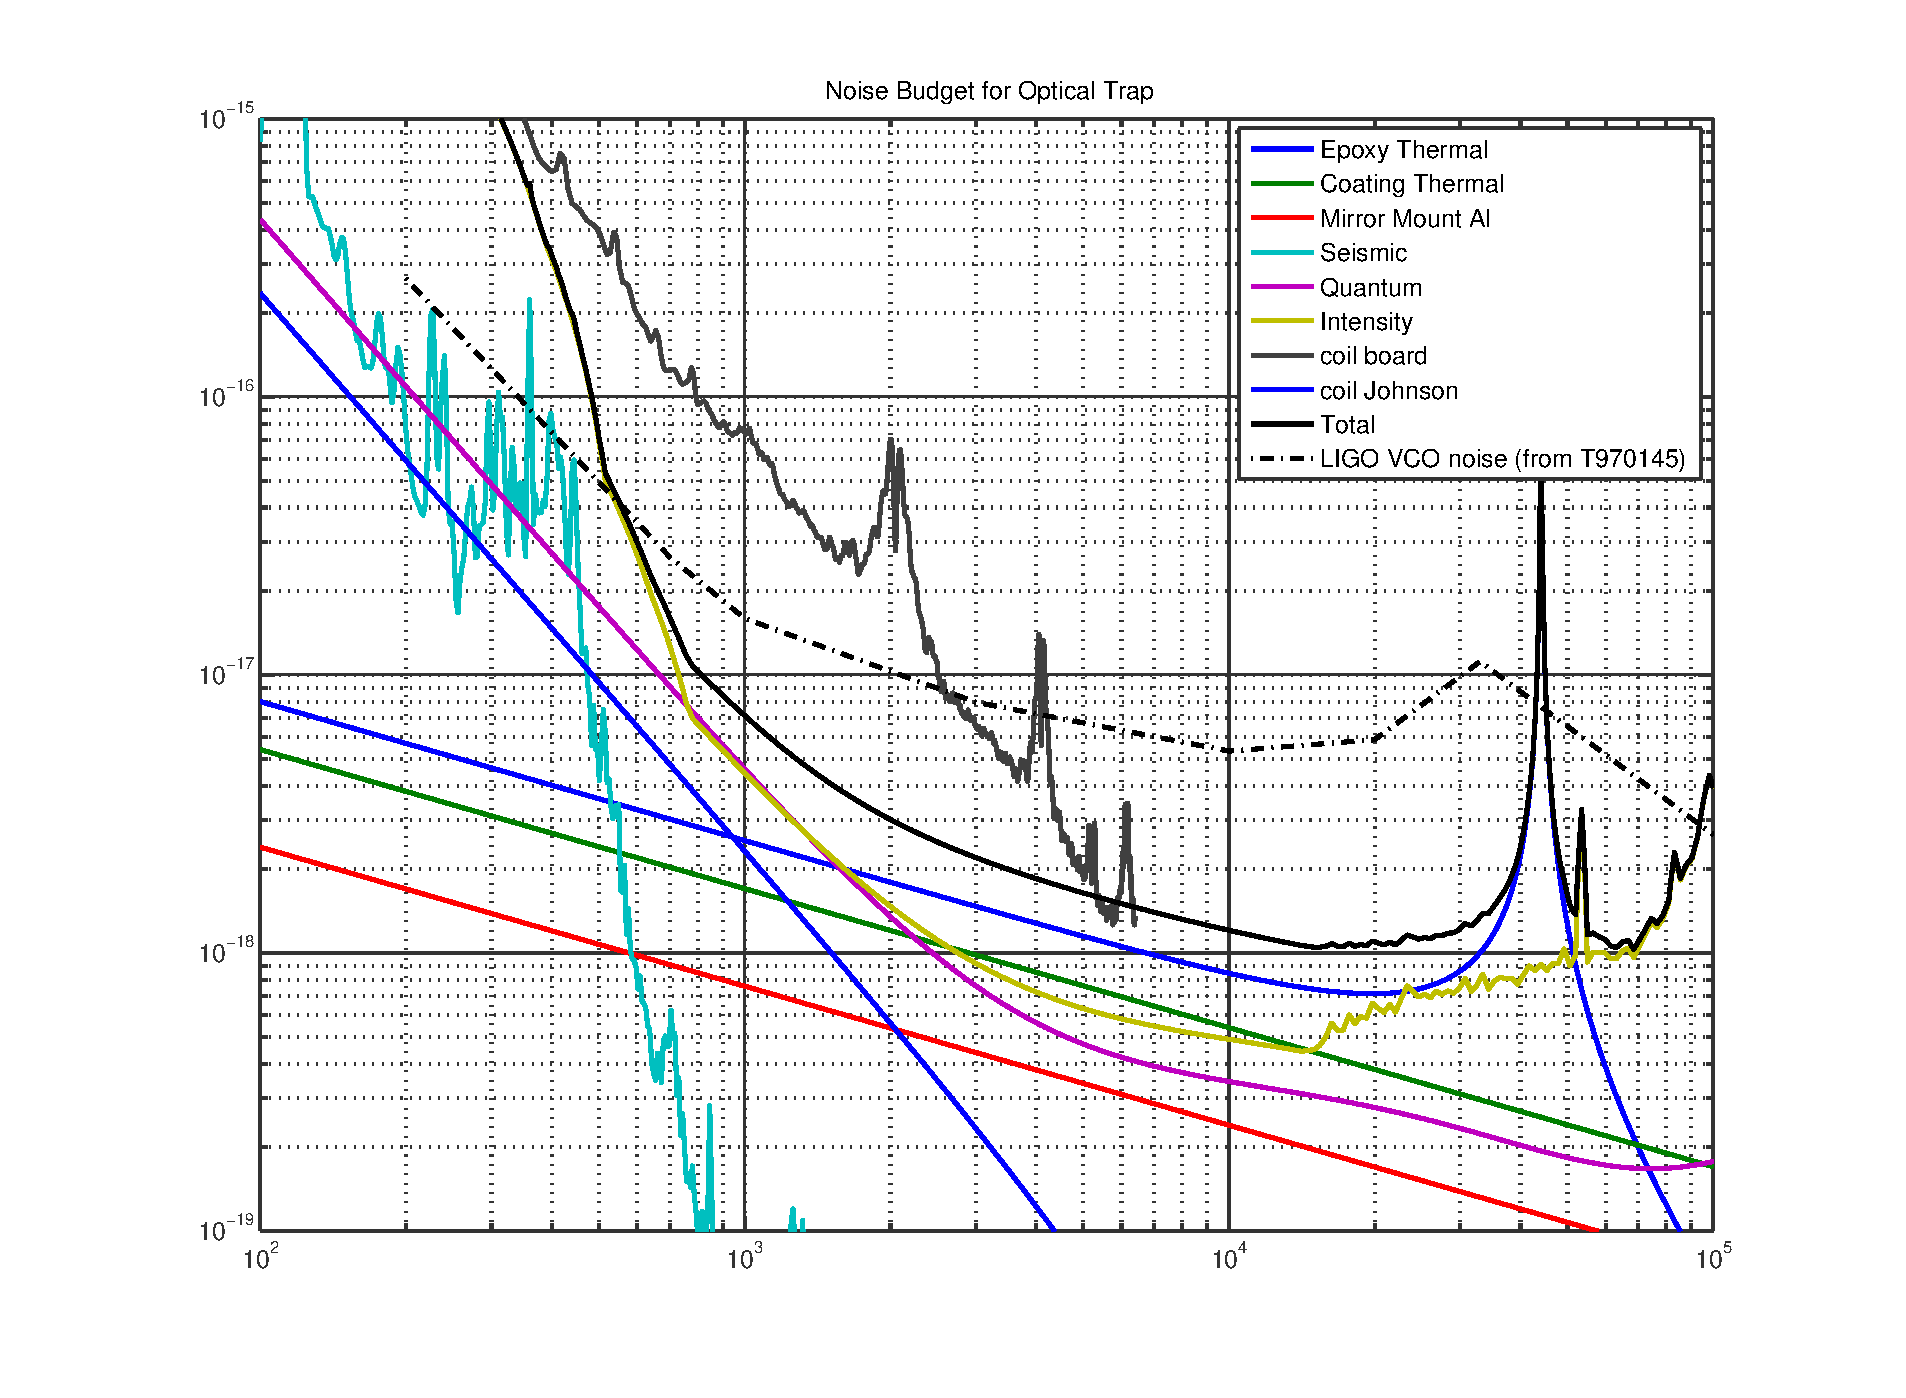
\includegraphics[width=15cm]{./figures/noise_budget.eps}
	\caption[Noise Budget]{Noise budget}
	\label{fig:noise_bud}
\end{figure}

\begin{figure}[htbp]
	\centering
		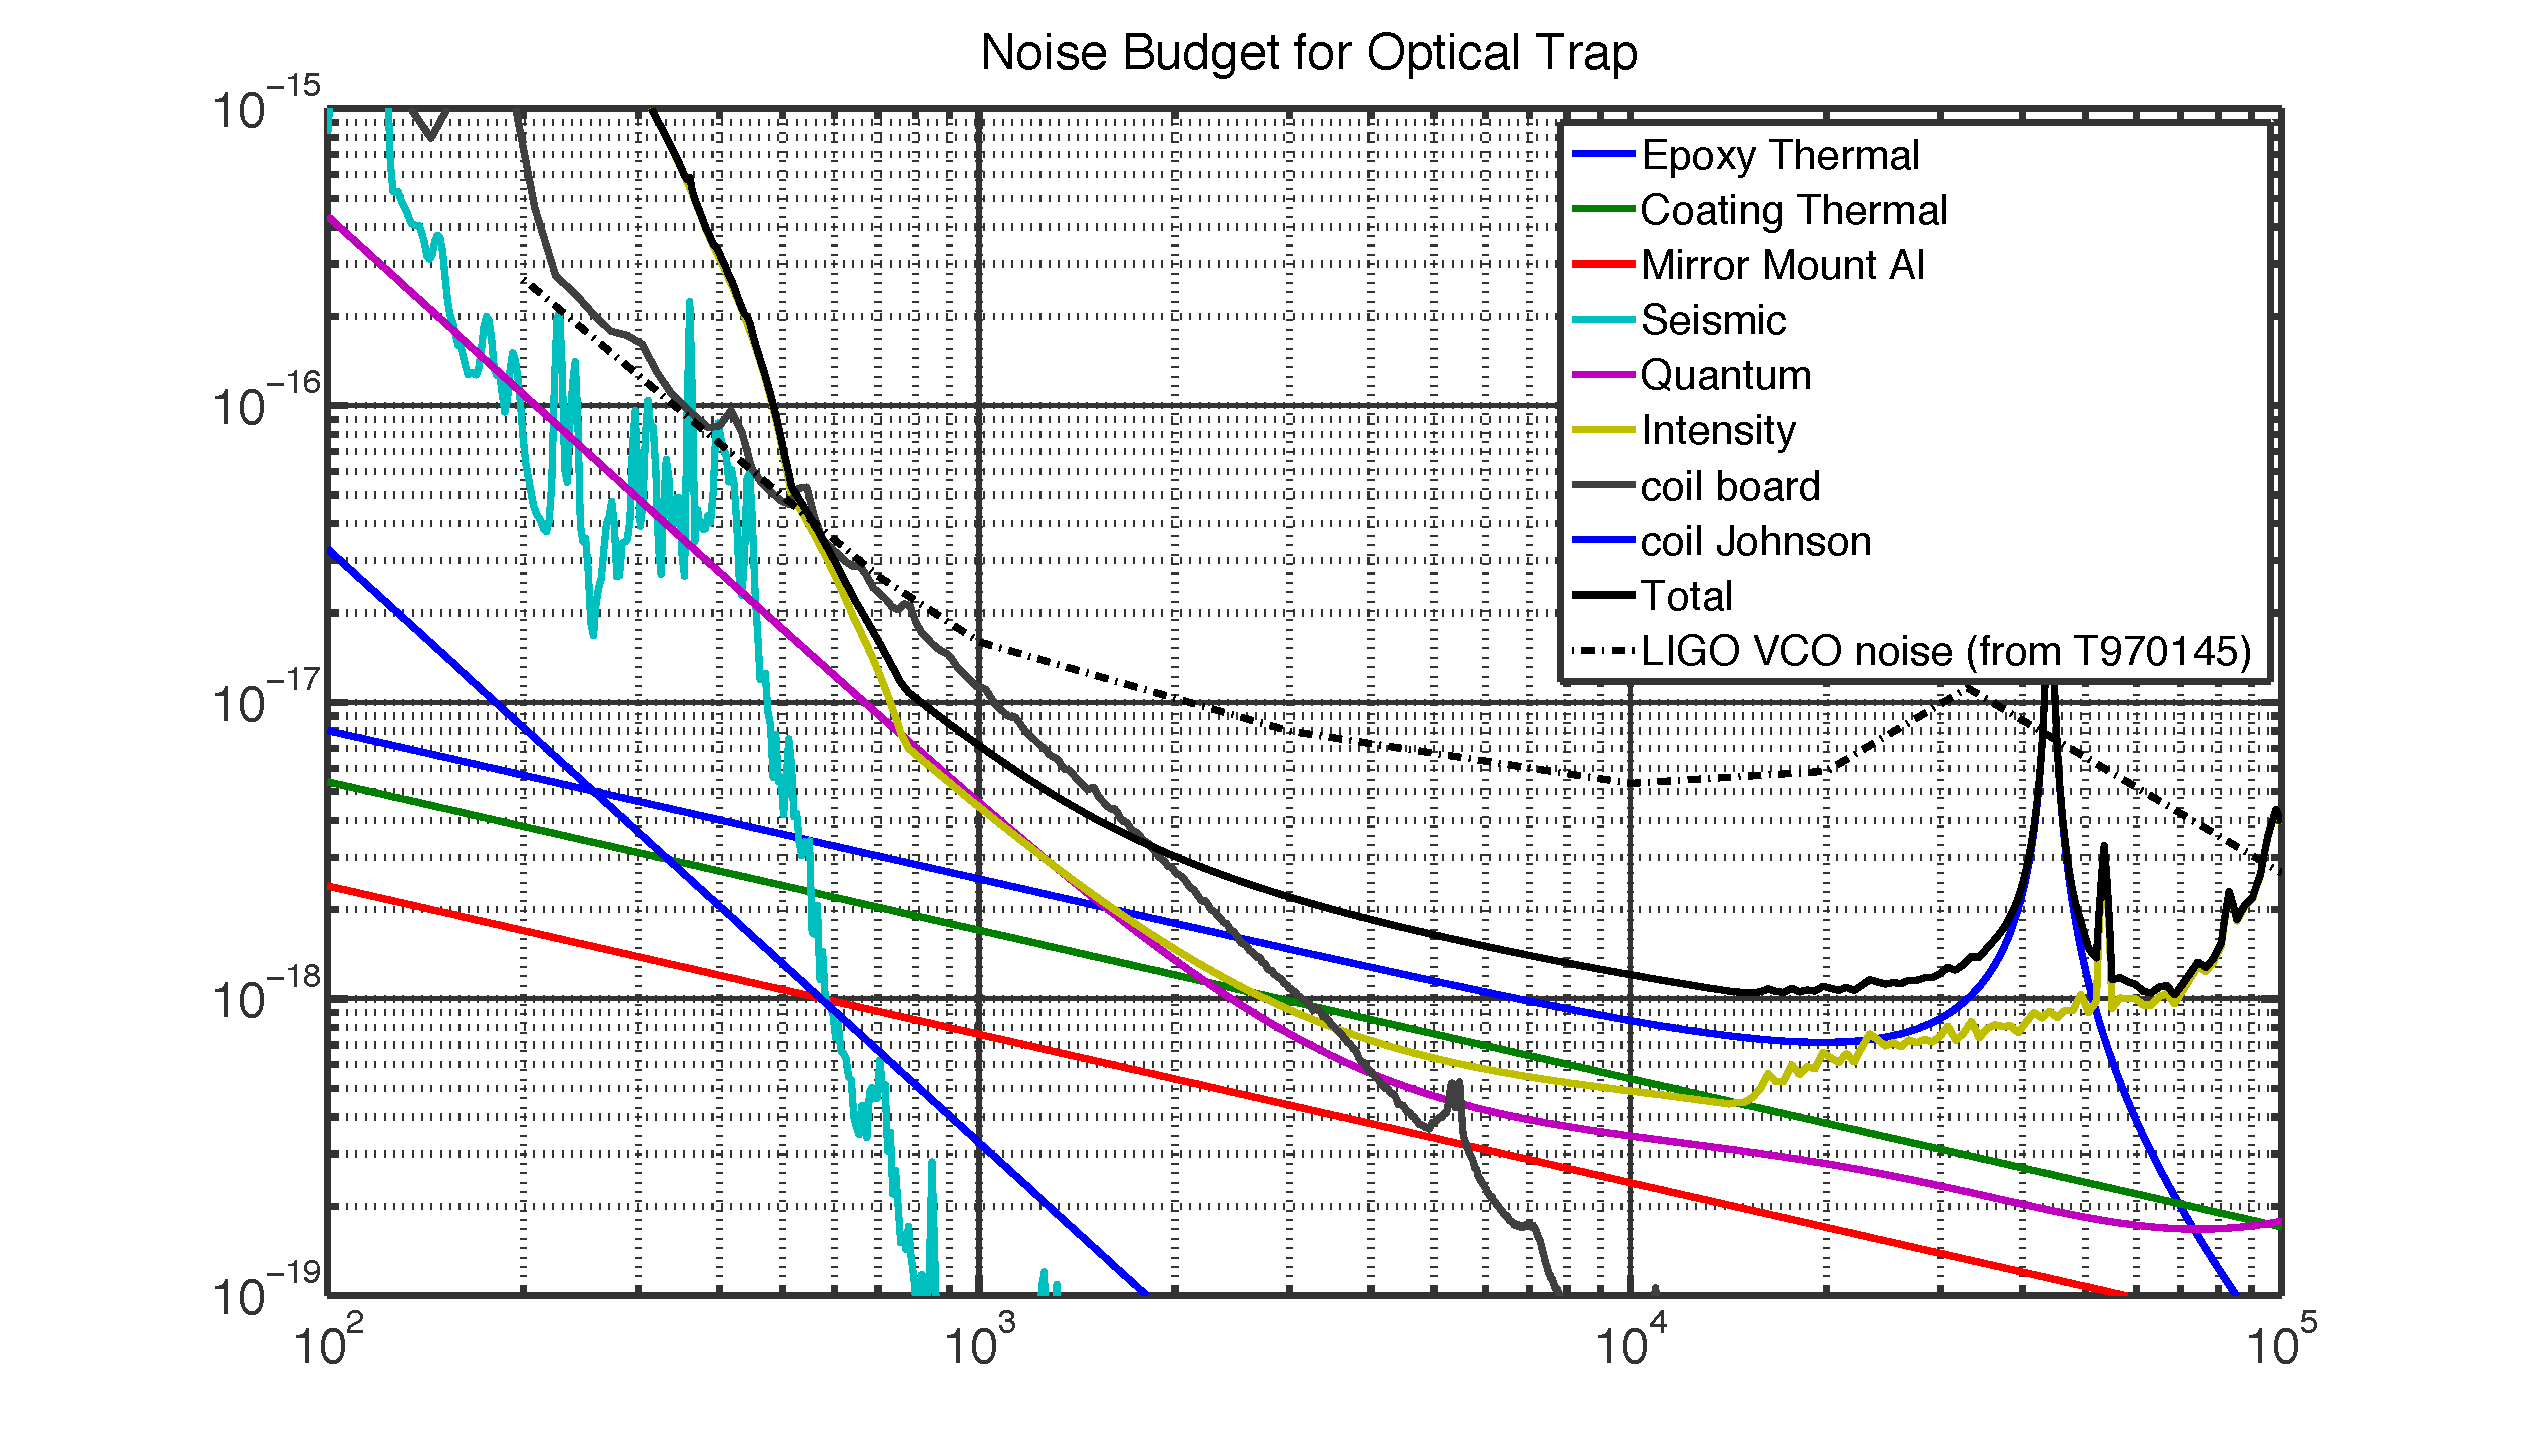
\includegraphics[width=15cm]{./figures/NoiseBudgetBoard.pdf}
	\caption[Noise Budget Board]{Noise budget with coil driver board noise}
	\label{fig:noise_bud_brd}
\end{figure}

\section{Vacuum Requirements for Optical Trap}

It is desired to have an understanding of limits of vacuum gas constituents for the in-vacuum experiment. From the LIGO DCC we have a few documents that describe the process that went into understanding the problem for 2 4km long Fabry-Perot cavities. I will apply these techniques to a 10-30cm cavity.\\


\subsection{LIGO Vacuum Requirements}

The amplitude spectral density of the optical path length is given by,

\begin{align*}
\Delta L ( f ) = 4 \pi \left( \frac{2 L_0 p}{k T w_0 v_0} \right)^{1/2} a e^{- \pi f w_0 / v_0 }
\end{align*} \\


From *** the value for $4 \pi a \left( \frac{2}{k T w_0 L_0 v_0} \right)^{1/2} $ is $ 4.8 x 10^{-21} \left( \frac{R_x}{R_{H_2}} \right) $. Where $L_0 = 4000 \mathrm{m} $ and $ w_0 = 0.06 \mathrm{m} $. \\

For our purposes (single arm cavity) we will lose a factor of $ \sqrt{2} $. \\

We end up with a formula for amplitude spectral density in a one-arm cavity that is:

\begin{align*}
\Delta L ( f ) = 4 \pi \left( 5.3 \mathrm{x} 10^{-20} \right) \left(  \frac{R_x}{R_{H_2}} \right) \sqrt{\frac{ L_0 p}{ w_0 } } e^{- \pi f w_0 / v_0 }
\end{align*} \\

\subsection{Optical Trap}

Now, we insert parameters for the cavity. For the first look, I use the parameters defined in the project description: 0.3m cavity length, 0.2m radius of curvature for each mirror.
\todo{something},

If we operate at a pressure of 1e-6 Torr, no constituent gas can be greater than this. The following plot is of constituent gases at this pressure.

\begin{figure}[htbp]
	\centering
		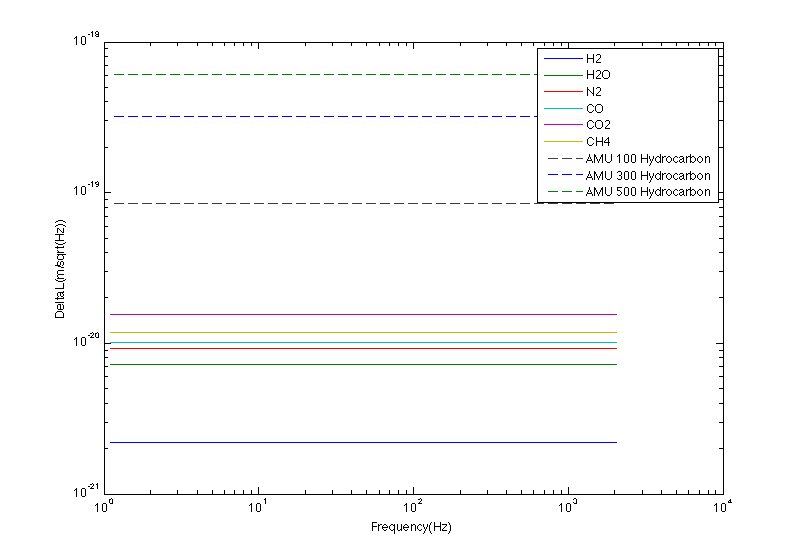
\includegraphics[width=15cm]{./figures/trapgasnoise_1.png}
	\caption[Gas Noise Comparison]{Gas Noise for 1e-6 Torr}
	\label{fig:gas_noise1}
\end{figure}

If we have a residual gas analyzer that detects a minimum partial pressure of 5e-11 Torr:

\begin{figure}[htbp]
	\centering
		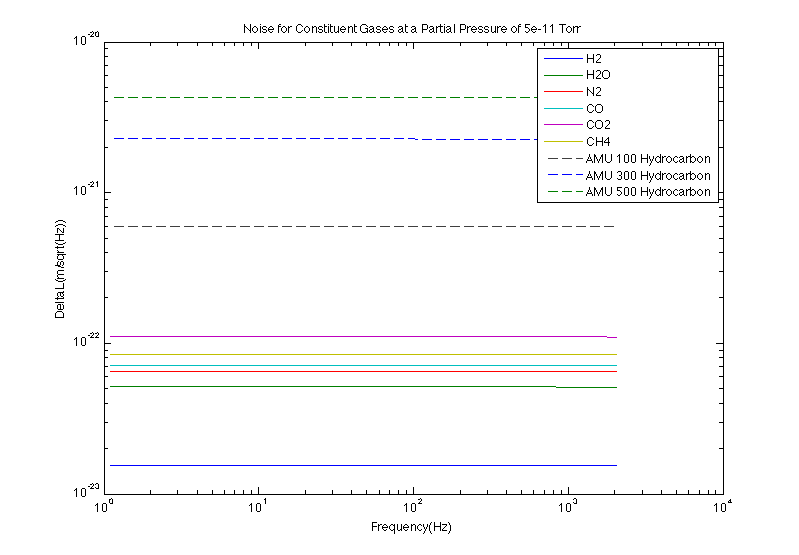
\includegraphics[width=15cm]{./figures/trapgasnoise_2.png}
	\caption[Gas Noise Comparison]{Gas Noise for 5e-11 Torr}
	\label{fig:gas_noise2}
\end{figure}

\section{Epoxy Thermal Noise}

Brownian thermal noise estimates for epoxy joints are gotten from basic application of the fluctuation-dissipation theorem. The form that we start with is,
\begin{align*}
S_{x^2}(f) = \frac{4 k_B T}{\omega^2} \Re(Z^{-1}), 
\end{align*}
where $Z$ is the impedance, $F / v$. The force equation that we use is of the form,
\begin{align*}
F_{\mathrm{ext}} = m \ddot{x} + k x,
\text{where k is a complex number}, (1 + i \phi)
\end{align*}

\section{Derivation}

\begin{align*}
d_n = d(t-\tau_n)
\end{align*} \\

\begin{align*}
d_n = d \left( t - \frac{(2n -1)}{c} L_0 - d_1 - \sum_{l=2}^{n} 2 d_l \right)
\end{align*} \\



\Chapter{Results}
\label{ch:results}
Linear trap measurements have been taken twice.
The first measurement was with the subcarrier at the same offset frequency from
the carrier for each measurement.
The results generally were in line with the theory, however there were
complications with the layout that we felt should be improved on.

\section{First Experiment}

%\begin{figure}[htbp]
%    \centering
%    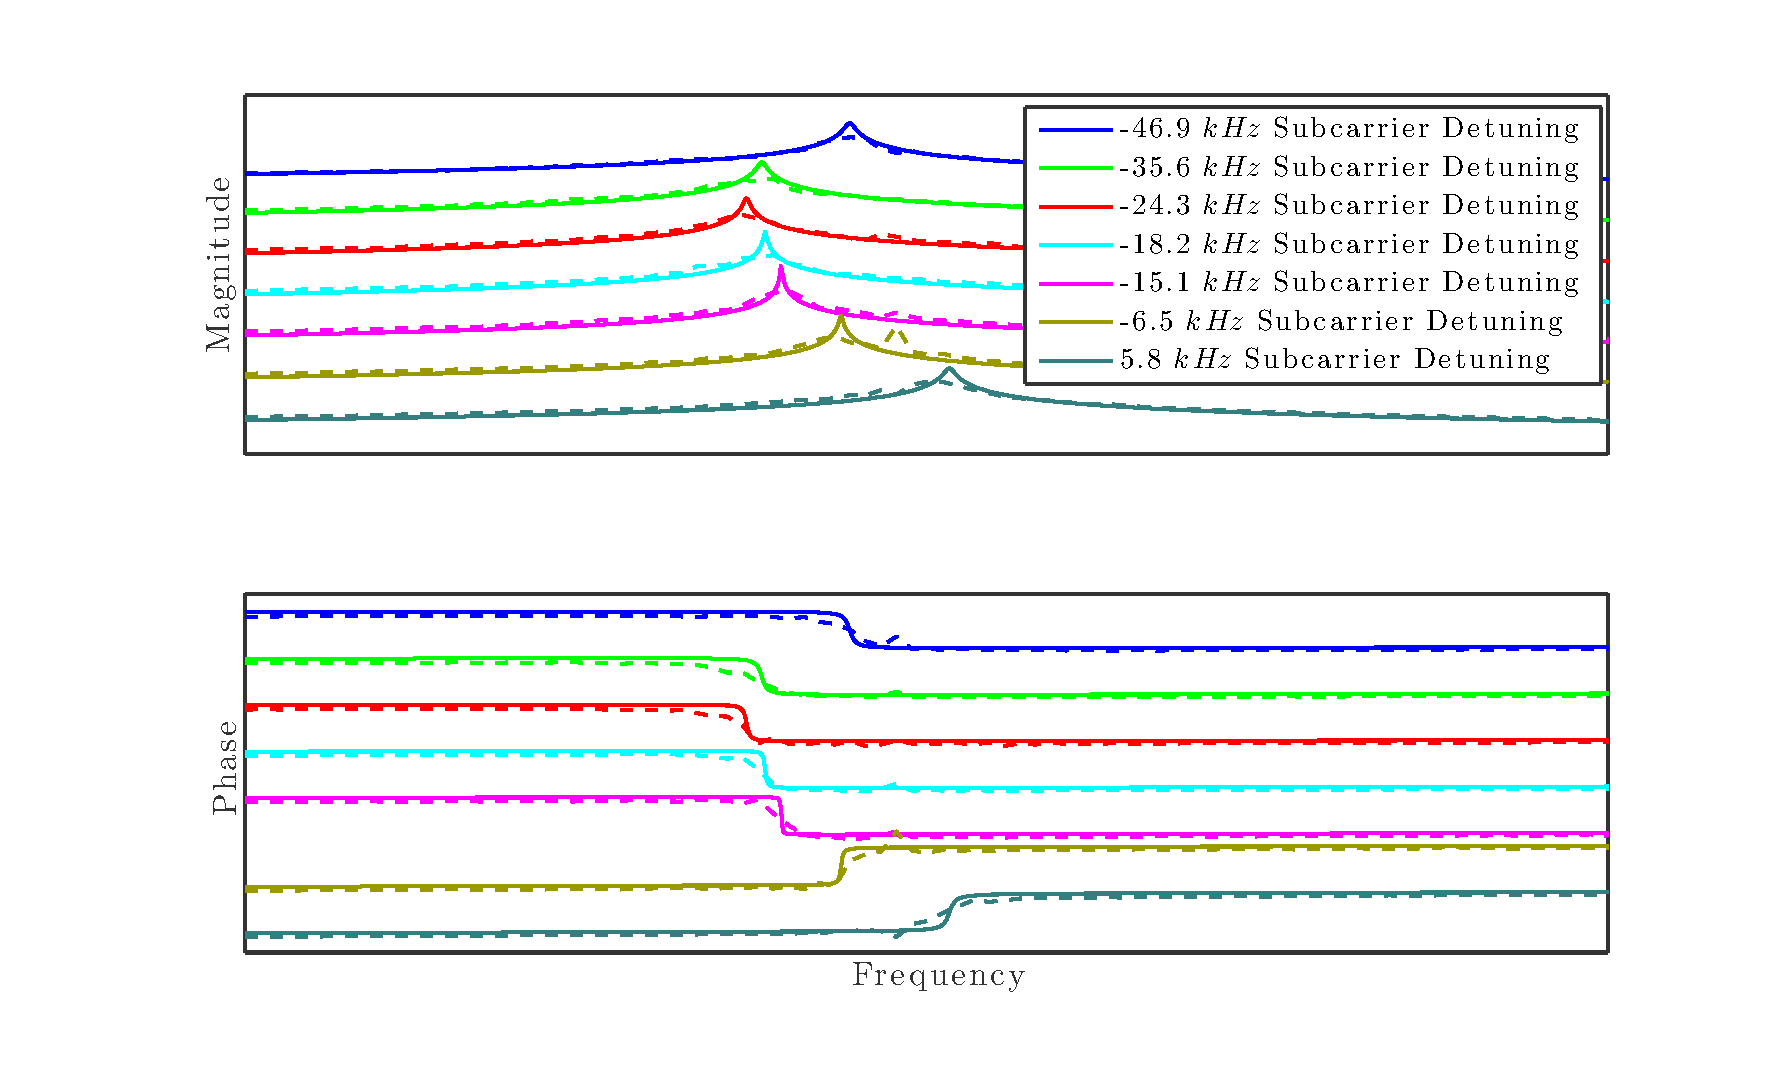
\includegraphics[width=20cm]{./figures/april_results_olgfit.eps}
%    \caption[Data Fitting of Open Loop Gain for 1st Results]{This is the open
%        loop gain fit of the last 7 measurements taken during a segment of
%        time in which the cavity was continuously locked.
%        The trap cavity had been locked for a few hours at this point and
%        seemed to have stabilized compared to earlier in the lock segment.
%        These measurements were taken no more than 5 minutes apart from each
%        other so the effects of any drifted were minimized.}
%    \label{fig:olgapril}
%\end{figure}

The first set of measurements seemed to have a large drift.
One of the reasons for this is the fact that the carrier beam was not
well aligned to the subcarrier beam causing drifts in the power ratio between
carrier and subcarrier as the overall alignment drifted.
Another complication in the first run was due to the fact that the carrier and
subcarrier beams had exactly the same polarizations which caused a strong
beat signal at $355kH\!z$. This beat signal was low enough in frequency that
it would show strongly in the resonant \ac{rfpd} output, likely causing
saturation effects in the electronics that would lead to an unpredictable
subcarrier detuning.

Despite these issues we were clearly able to observe
stable and unstable optical springs and there was a short stretch of
measurements that did line up with the model with certain assumptions
about the parameter space.


\begin{figure}[htbp]
  \label{fig:april_space1}
  \tikzsetnextfilename{april_space1}
  \begin{tikzpicture}
  \begin{axis}[
    name=plot1,
    height=8cm,
    width=14cm,
    ylabel={Resonant Frequency $(H\!z)$},
    xlabel={Subcarrier Detuning $(kH\!z)$},
    grid=major,
  ]
  \addplot[blue,very thick] table[x index=1,y index=2]
    {./matlab_traces/april_fitspace_stable.dat};
  \addplot[green,very thick] table[x index=1,y index=2]
    {./matlab_traces/april_fitspace_unstable.dat};
  \addplot[blue,only marks] table[x index=1,y index=2]
    {./matlab_traces/april_pointspace_stable.dat};
  \addplot[green,only marks] table[x index=1,y index=2]
    {./matlab_traces/april_pointspace_unstable.dat};
  \end{axis}
  \end{tikzpicture}
  \caption[Parameters from 1st Experiment]{The solid lines show the theoretical
    spring frequencies for all of the measurements that took place in a span
    of about 30 minutes during the first experiment at the end of one lock
    stretch.
    The dots correspond to the actual measurements of the optical spring at
    different subcarrier detunings. The entire space depicted is in the region
    of static stability, i.e. the optical spring provides a restoring force.
    The colors correspond to the dynamic stability of the optical spring.
    Blue is dynamically stable.
    Green is dynamically unstable.
    The carrier frequency remained at a fixed offset from the subcarrier at
    $355\, kH\!z$.
    }
\end{figure}

\begin{figure}[htbp]
  \label{fig:april_olg1}
  \tikzsetnextfilename{april_olg1}
  \begin{tikzpicture}
  \begin{semilogyaxis}[
    name=plot1,
    height=5cm,
    width=7cm,
    xmin=760,
    xmax=880,
    ylabel={Magnitude},
    grid=major,
  ]
  \addplot[blue,very thick] table[x index=0,y index=1] {./matlab_traces/april_olg_38.dat};
  \addplot[blue] table[x index=0,y index=1] {./matlab_traces/april_fit.dat};
  \addplot[red,very thick] table[x index=0,y index=1] {./matlab_traces/april_olg_39.dat};
  \addplot[red] table[x index=0,y index=3] {./matlab_traces/april_fit.dat};
  \addplot[green,very thick] table[x index=0,y index=1] {./matlab_traces/april_olg_40.dat};
  \addplot[green] table[x index=0,y index=5] {./matlab_traces/april_fit.dat};
  \end{semilogyaxis}

  \begin{semilogyaxis}[
    name=plot2,
    at=(plot1.below south), anchor=above north,
    height=5cm,
    width=7cm,
    xmin=760,
    xmax=880,
    xlabel={Frequency $(H\!z)$},
    ylabel={Magnitude},
    grid=major,
  ]
  \addplot[blue,very thick] table[x index=0,y index=1] {./matlab_traces/april_olg_41.dat};
  \addplot[blue] table[x index=0,y index=7] {./matlab_traces/april_fit.dat};
  \addplot[red,very thick] table[x index=0,y index=1] {./matlab_traces/april_olg_42.dat};
  \addplot[red] table[x index=0,y index=9] {./matlab_traces/april_fit.dat};
  \addplot[green,very thick] table[x index=0,y index=1] {./matlab_traces/april_olg_43.dat};
  \addplot[green] table[x index=0,y index=11] {./matlab_traces/april_fit.dat};
  \addplot[black,very thick] table[x index=0,y index=1] {./matlab_traces/april_olg_44.dat};
  \addplot[black] table[x index=0,y index=13] {./matlab_traces/april_fit.dat};
  \end{semilogyaxis}

  \begin{axis}[
    name=plot3,
    at=(plot1.right of east), anchor=left of west,
    height=5cm,
    width=7cm,
    xmin=760,
    xmax=880,
    ylabel={Phase},
    grid=major,
  ]
  \addplot[blue,very thick] table[x index=0,y index=2] {./matlab_traces/april_olg_38.dat};
  \addplot[blue] table[x index=0,y index=2] {./matlab_traces/april_fit.dat};
  \addplot[red,very thick] table[x index=0,y index=2] {./matlab_traces/april_olg_39.dat};
  \addplot[red] table[x index=0,y index=4] {./matlab_traces/april_fit.dat};
  \addplot[green,very thick] table[x index=0,y index=2] {./matlab_traces/april_olg_40.dat};
  \addplot[green] table[x index=0,y index=6] {./matlab_traces/april_fit.dat};
  \end{axis}
  \begin{axis}[
    name=plot4,
    at=(plot2.right of east), anchor=left of west,
    height=5cm,
    width=7cm,
    xmin=760,
    xmax=880,
    xlabel={Frequency $(H\!z)$},
    ylabel={Phase},
    grid=major,
  ]
  \addplot[blue,very thick] table[x index=0,y index=2] {./matlab_traces/april_olg_41.dat};
  \addplot[blue] table[x index=0,y index=8] {./matlab_traces/april_fit.dat};
  \addplot[red,very thick] table[x index=0,y index=2] {./matlab_traces/april_olg_42.dat};
  \addplot[red] table[x index=0,y index=10] {./matlab_traces/april_fit.dat};
  \addplot[green,very thick] table[x index=0,y index=2] {./matlab_traces/april_olg_43.dat};
  \addplot[green] table[x index=0,y index=12] {./matlab_traces/april_fit.dat};
  \addplot[black,very thick] table[x index=0,y index=2] {./matlab_traces/april_olg_44.dat};
  \addplot[black] table[x index=0,y index=14] {./matlab_traces/april_fit.dat};
  \end{axis}
  \end{tikzpicture}
    \caption[Data Fitting of Open Loop Gain for 1st Results]{This is the open
        loop gain fit of the last 7 measurements taken during a segment of
        time in which the cavity was continuously locked.
        The three traces in the top two plots are of the stable spring with
        a large negative detuning.
        They correspond to the three blue dots from figure
        \ref{fig:april_space1} with the most negative subcarrier detuning.
        The thick traces in all plots are from the measurements in the lab.
        The thin traces are of the modelled open loop gain.
        The trap cavity had been locked for a few hours at this point and
        seemed to have stabilized compared to earlier in the lock segment.
        These measurements were taken no more than 5 minutes apart from each
        other so the effects of any drifting were minimized.}
  \label{fig:aprilolg1}
\end{figure}


\section{Experimental Layout Revision}
From our first layout design there was a rather
large beat signal on the \ac{rfpd} used for generating the \ac{pdh} signal
for our locking feedback servo.
This beat signal is a result of our initial layout involving the combining of
carrier and subcarrier beams before the \ac{fi} which resulted in the two beams
having the same polarization.
This produces a beat signal of the difference in the two frequencies.
The beat signal shows up in our resonant \ac{rfpd} because we use a small
frequency offset.
We feared there could be saturations in the photodiode electronics that would
cause unpredictable electronic offsets in the trap locking feedback servo
resulting in an error on the subcarrier detuning lock point.


\section{Second Experiment}

During the second experiment we were able to observe several stable and
unstable spring as before. This time we varied the frequency offset between
carrier and subcarrier for each measurement, keeping the other settings
fixed.

We ran into some complications while fitting the data.
The stability of the optical springs would not match with the theory without
the addition of some extra physics.
With the addition of an effect from the thermal expansion of the high
reflective optical coatings, we were able to fit the stablility
properly.

Thermal expansion couples in to the transfer function by the fact that driving
the position of the mirror causes a power fluctuation and thus a temperature
fluctuation in the surface of the mirror due to absorption.
This temperature fluctuation causes a fluctuation in the thickness
of the optic.
This will be expained in more detail in section
\ref{sec:opticthermalexpansion}.
It turns out that only 5ppm absorption is required to account for the
discrepancy in stablility.
This is, in part, due to the high circulating power and the small
beam spot size on the cavity end mirrors.
The results of this fitting can be seen in figure \ref{fig:juneOLGresults}.

\subsection{Optic Thermal Expansion Contribution}
\label{sec:opticthermalexpansion}
See section 2.8.5 of Stefan Ballmer's thesis  \cite{Ballmer:thesis} for
a thorough discussion on thermal noise couplings.
The relevant part that we are interested in is the effect of changing
the thickness of the optic itself due to thermal expansion.
We want to first consider the penetration depth $d$ of the thermal
fluctuations. This is given by,
\begin{align}
d &= \sqrt{\frac{\kappa}{2\pi fC\rho}} = 50\mu m \sqrt{\frac{400 H\!z}{f}}
\end{align}
This is nearly an order of magnitude smaller than the beam spot diameter, which
is about $320\mu m$. The change in thickness $\Delta_z$ of the optic can then
be approximated with,
\begin{align}
\Delta_z &= \left(1+\eta\right)\alpha\frac{ \delta P(f) }{2\pi ifC\rho A}
\end{align}
where $\delta$ is the absorption coefficient, $A$ is the area of the beam,
and $\eta$ is the Poisson ratio.

The majority of the change in power buildup due to cavity length is due to the
carrier beam which has a positive detuning.
Because of this detuning, expansion of the optics will shorten the cavity and
increase the intracavity power.
The intracavity power fluctuations will thus have a positive feedback and add
to the instability of the optical spring.


\begin{figure}[htbp]
  \tikzsetnextfilename{juneOLGresults}
  \begin{tikzpicture}
  \begin{loglogaxis}[
    name=plot1,
    height=7cm,
    width=14cm,
    xmin=100,
    xmax=2000,
    xtick={1e2,1e3},
    ylabel={Magnitude},
    grid=both,
  ]
  \addplot[blue,very thick,dashed] table[x index=0,y index=1]
    {./matlab_traces/juneResults13fit.dat};
  \addplot[green,very thick,dashed] table[x index=0,y index=1]
    {./matlab_traces/juneResults20fit.dat};
  \addplot[red,very thick,dashed] table[x index=0,y index=1]
    {./matlab_traces/juneResults10fit.dat};
  \addplot[teal,very thick,dashed] table[x index=0,y index=1]
    {./matlab_traces/juneResults15fit.dat};
  \addplot[magenta,very thick,dashed] table[x index=0,y index=1]
    {./matlab_traces/juneResults18fit.dat};
  \addplot[yellow,very thick,dashed] table[x index=0,y index=1]
    {./matlab_traces/juneResults19fit.dat};
  \addplot[blue,very thick] table[x index=0,y index=1] {./matlab_traces/juneResults13.dat};
  \addplot[green,very thick] table[x index=0,y index=1] {./matlab_traces/juneResults20.dat};
  \addplot[red,very thick] table[x index=0,y index=1] {./matlab_traces/juneResults10.dat};
  \addplot[teal,very thick] table[x index=0,y index=1] {./matlab_traces/juneResults15.dat};
  \addplot[magenta,very thick] table[x index=0,y index=1] {./matlab_traces/juneResults18.dat};
  \addplot[yellow,very thick] table[x index=0,y index=1] {./matlab_traces/juneResults19.dat};
  \end{loglogaxis}
  \begin{semilogxaxis}[
    name=plot2,
    at=(plot1.below south), anchor=above north,
    height=7cm,
    width=14cm,
    xmin=100,
    xmax=2000,
    xtick={1e2,1e3},
    xlabel={Frequency $(H\!z)$},
    ylabel={Phase (Deg)},
    legend style={legend pos=north west,font=\tiny},
    grid=both,
  ]
  \addplot[blue,very thick,dashed,forget plot] table[x index=0,y index=2]
    {./matlab_traces/juneResults13fit.dat};
  \addplot[green,very thick,dashed,forget plot] table[x index=0,y index=2]
    {./matlab_traces/juneResults20fit.dat};
  \addplot[red,very thick,dashed,forget plot] table[x index=0,y index=2]
    {./matlab_traces/juneResults10fit.dat};
  \addplot[teal,very thick,dashed,forget plot] table[x index=0,y index=2]
    {./matlab_traces/juneResults15fit.dat};
  \addplot[magenta,very thick,dashed,forget plot] table[x index=0,y index=2]
    {./matlab_traces/juneResults18fit.dat};
  \addplot[yellow,very thick,dashed,forget plot] table[x index=0,y index=2]
    {./matlab_traces/juneResults19fit.dat};
  \addplot[blue,very thick] table[x index=0,y index=2] {./matlab_traces/juneResults13.dat};
  \addlegendentry{DetC$=290.8kH\!z$,DetS$=-39.2kH\!z$,Pratio=3.46}
  \addplot[green,very thick] table[x index=0,y index=2] {./matlab_traces/juneResults20.dat};
  \addlegendentry{DetC$=285.0kH\!z$,DetS$=-45.0kH\!z$,Pratio=3.96}
  \addplot[red,very thick] table[x index=0,y index=2] {./matlab_traces/juneResults10.dat};
  \addlegendentry{DetC$=285.1kH\!z$,DetS$=-34.9kH\!z$,Pratio=3.50}
  \addplot[teal,very thick] table[x index=0,y index=2] {./matlab_traces/juneResults15.dat};
  \addlegendentry{DetC$=264.2kH\!z$,DetS$=-35.8kH\!z$,Pratio=3.94}
  \addplot[magenta,very thick] table[x index=0,y index=2] {./matlab_traces/juneResults18.dat};
  \addlegendentry{DetC$=238.2kH\!z$,DetS$=-21.8kH\!z$,Pratio=4.27}
  \addplot[yellow,very thick] table[x index=0,y index=2] {./matlab_traces/juneResults19.dat};
  \addlegendentry{DetC$=222.5kH\!z$,DetS$=-17.5kH\!z$,Pratio=4.42}
  \end{semilogxaxis}
  \end{tikzpicture}
    \caption[Data Fitting of Open Loop Gain for 1st Results]{This is the open
      loop gain fit for the second experiment. The solid lines are the measured
      optical spring transfer functions. The dashed lines are the corresponding
      theoretical transfer functions. In the legend, "DetC" and "DetS" stand for
      carrier and subcarrier detuning respectively. Pratio is the power ratio
      of carrier to subcarrier input power.}
  \label{fig:juneOLGresults}
\end{figure}


\begin{figure}[htbp]
  \tikzsetnextfilename{noisepassive}
  \begin{tikzpicture}
  \begin{loglogaxis}[
    height=12cm,
    width=14cm,
    xlabel={Frequency $(H\!z)$},
    ylabel={Trap Length Noise $(m/\sqrt{H\!z})$},
    xmin=10,
    xmax=6000,
    ymin=1e-16,
    ymax=1e-8,
    grid=major,
    legend cell align=left,
  ]
  \addplot[blue,very thick] table[x index=0,y index=1]
    {./matlab_traces/june_noises.dat};
  \addlegendentry{Measured Trap Length Noise}
  \addplot[red,very thick] table[x index=0,y index=5]
    {./matlab_traces/june_noises.dat};
  \addlegendentry{Trap Length Noise Without Active Feedback}
  \addplot[red,dashed,very thick] table[x index=0,y index=6]
    {./matlab_traces/june_noises.dat};
  \addlegendentry{Trap Length RMS Without Active Feedback}
  \end{loglogaxis}
  \end{tikzpicture}
  \caption[Estimate of Passively Attenuated Noise]{This is the noise budget which includes the measured
    cavity length noise with a stable optical spring.}
  \label{fig:noisepassive}
\end{figure}




\Chapter{Digital System}
\label{ch:digital}

%%%%%%%%%%
\section{System Overview}

In order to provide control of our small optic suspensions, we had the option of building either a digital or analog feedback system.
Although either option would work for the experiment the digital system provides additional benifits:

\begin{enumerate}
\item Easy modification of feedback loops
\item Builds Familiarity to LIGO digital systems
\item Can be used as a platform for testing new LIGO tools
\item A platform for rapid implementation of future control loops
\end{enumerate}

The digital system employed at Syracuse closely resembles the LIGO digital system. It is composed of the following major components:
\begin{enumerate}
\item Real-time Front-end for digital feedback and control
\item ADC and DAC for interfacing digital system with the experiment
\item Data Acquisition
\item Workstation for controlling the experiment, running tests, and analyzing data
\item Boot server for serving the diskless front-end machine
\end{enumerate}

\begin{figure}[htbp]
	\centering
		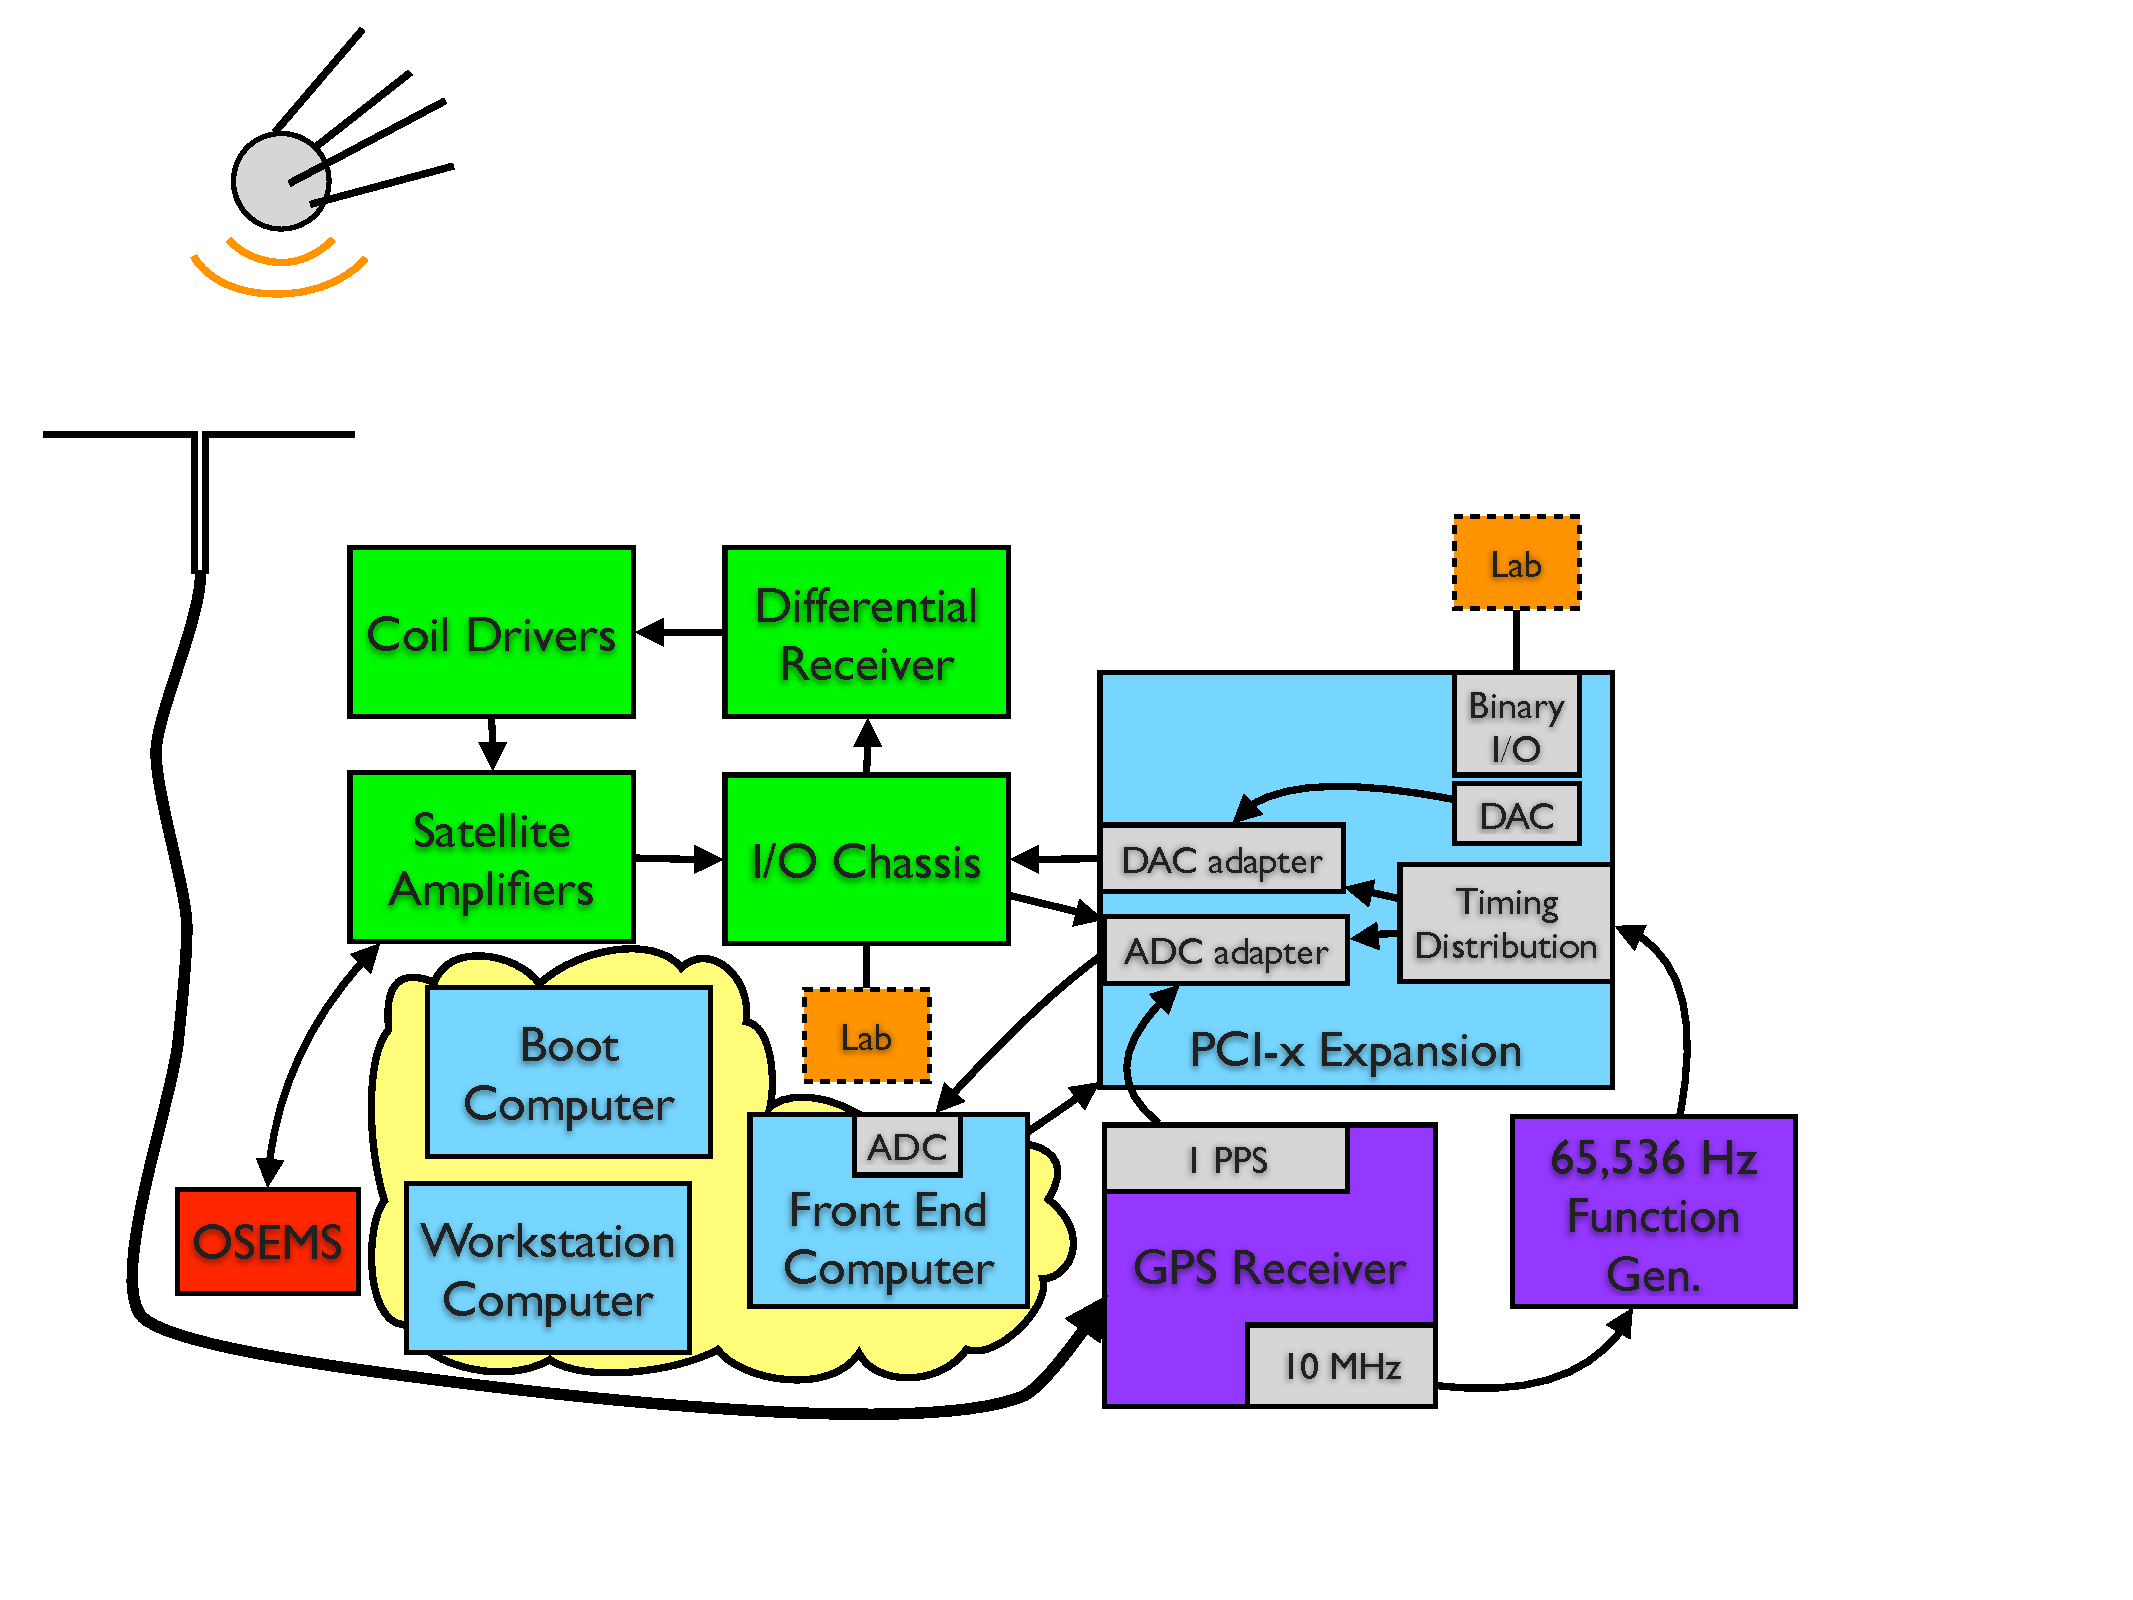
\includegraphics[width=15cm]{./figures/FrontEndSystem.pdf}
	\caption[Front End System Overview]{Front End System Overview}
	\label{fig:front_end}
\end{figure}

\begin{table}
\begin{center}
\begin{tabular}{ | l | l | l | }
\hline
From & To & Connection \\
\hline
Front-End Computer & ADC card & PCIe bus \\
Front-End Computer & Expansion Chassis & PCIe to PCIx adapter \\
Expansion Chassis & DAC card & PCIx bus \\
ADC card & ADC adapter card & SCSI cable \\
DAC card & DAC adapter card & SCSI cable \\
Expansion Chassis & Binary I/O cards & PCIx bus \\
Timing Distribution Card & ADC card & coaxial SMB \\
Timing Distribution Card & DAC card & coaxial SMB \\
Function Generator & Timing Distribution Card & BNC \\
GPS Receiver & Function Generator & 10 MHz sync BNC \\
GPS Receiver & ADC adapter card & 1PPS BNC \\
\hline
\end{tabular}
\end{center}
\caption[Digital System Hardware Interface Matrix]{This interface matrix depicts
the physical interconnectivity of digital system hardware components.
}
\end{table}

%%%%%
\subsection{LIGO Real-Time System Theory of Operation}

The LIGO Real-Time System provides for discrete, synchronous control of LIGO
systems. The sampling frequency can be one of several powers of 2 in Hz.
Time is synchronized to GPS time with a sophisticated timing distribution
system. The digital processes are run in fixed time steps in order to run
feedback signals through them which are analogous to continuous time feedback
systems. One can then design a feedback system composed of poles and zeros
completely inside the computer. The limitation being that of a bandwidth below
the Nyquist frequency for the sampling rate used.

Timing signals are received by the digital system through the ADC/DAC cards.
Each model is an individual process which has a limited time to process its
data before the next time step begins. Interprocess communication happens at
the beginning/end of each time step.


%%%%%
\subsection{ADC/DAC Hardware Description}

%%%%%
\subsection{Timing}

Time steps must be spaced precisely enough to avoid jitter (a phase noise
associated with a variable time step). In practice it is impossible to
avoid, but we can minimize jitter by referencing a crystal oscillator.
Crystal oscillators are notoriously precise by using the natural mechanical 
oscillations of crystals which have very low mechanical loss.

The timing signal for the front end system is directly generated by a Stanford Research DS345 function generator. It produces a 65,536 Hz signal that clocks the ADC and DAC cards. Over a long period of time the time stamp in the front end can drift relative to the computers that are synced to network time. Some software, particularly Diagnostic Test Tools and probably others, gets confused when the current time in front end does not match network time. This requires a reboot of the front end system to reacquire the correct time.

We ordered a GPS receiver (Trimble Thunderbolt E) that will prevent these long term drifts. It produces a 1PPS (Pulse Per Second) signal and a 10 MHz signal. The 1PPS connects to the ADC card through the ADC adapter card which is located in the blue expansion chassis. The 10 MHz signal connects to the external timebase input of the DS345. So, the 65,536 clock is now "disciplined" to the GPS time and as such should not drift over long periods of time.

Additionally, the Thunderbolt has an ovenized crystal oscillator that should help with phase noise.

In order to get the GPS antenna signal we needed about 250' of low-loss 1/2" diameter foam core cable (should be easy to spot as it's quite thick). The cable runs out the optics lab, across the hallway overhead and into a cable tray to go down the hallway. The cable runs out of the cable tray by the machine shop, over the hallway, into the machine shop, up to the ceiling, and then along the top of a black drain pipe to the south-east corner of the building. The cable then goes through some grating on the wall and up the shaft to the ground level of the SE corner where the antenna is mounted. (see Fig.\ref{fig:gps_antenna})

\begin{figure}[htbp]
	\centering
		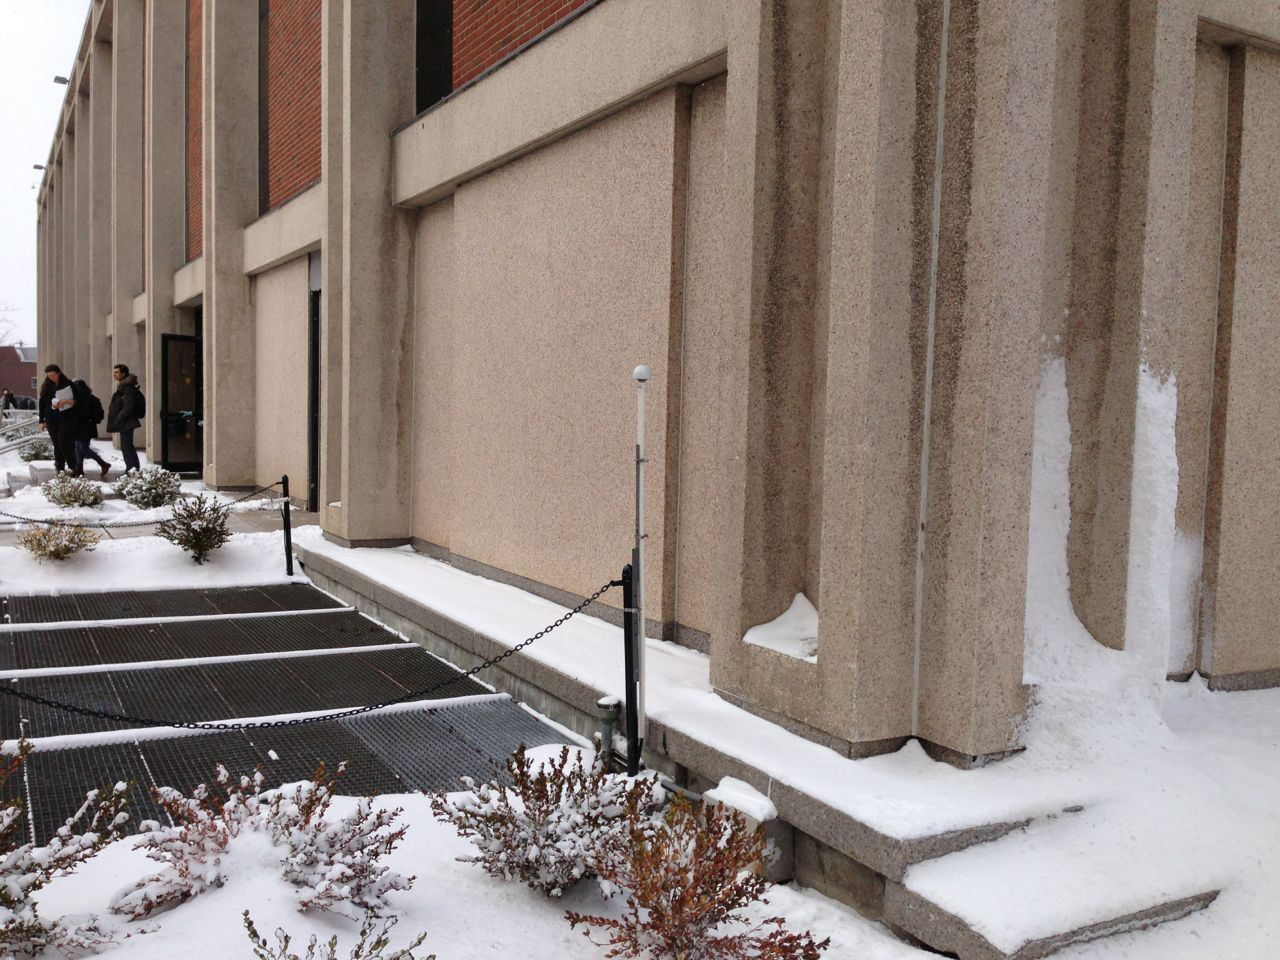
\includegraphics[width=15cm]{./figures/IMG_1308.jpg}
	\caption[GPS Antenna Location]{The GPS antenna is located }
	\label{fig:gps_antenna}
\end{figure}

The 1PPS signal from the Trimble Thunderbolt GPS receiver is a fixed pulse width of 10 micro-seconds. Since the clock is running at 65,536 Hz, the 1PPS is missed by the ADC.

I have fixed this by extending the pulse to about 15 microseconds using a 555 timer chip in monostable mode. The input has to be an inverse pulse so I inverted the pulse in GPS control software. This option is available in the Timing Receiver Configuration window.

See attached NE555P spec sheet (p.9) for the schematic that I used. Only difference is $R_L$ is between output and ground instead of $V_{CC}$.

I scavenged a 5V power supply from an old 10baseT ethernet hub. I took the ferrites and electrolytic capacitor that were on the supply input in the hub itself and added them to this board for noise suppression.

$R_A$ is a small potentiometer. If you need to adjust the pulse width, just open the case and turn the pot. Clockwise increases the width.

\begin{figure}[htbp]
	\centering
		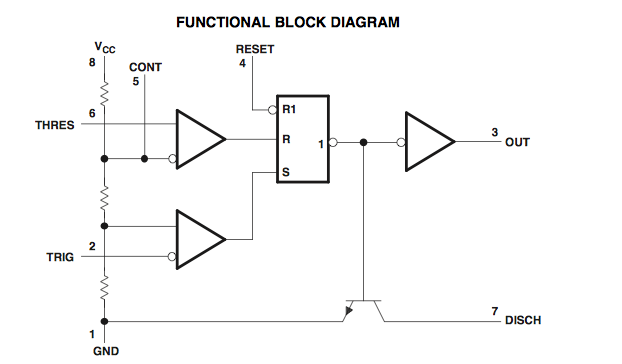
\includegraphics[width=15cm]{./figures/timer555.png}
	\caption[555 Timer Diagram]{This block diagram depicts the function of the 555 timer. The }
	\label{fig:timer_diag}
\end{figure}


\begin{figure}[htbp]
	\centering
		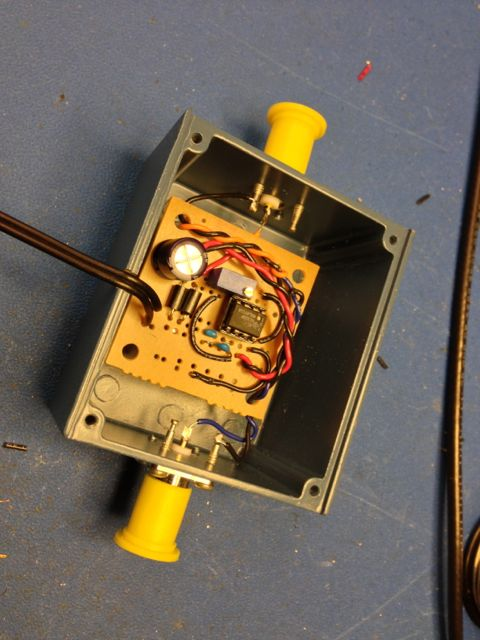
\includegraphics[width=15cm]{./figures/IMG_1345.jpg}
	\caption{{GPS Pulse Extender}}
	\label{fig:gps_pulse}
\end{figure}

The first thing to check in the GPS software is the status. It should say "over-determined clock". Other key items in the control software to pay attention to are basically the number of green lights (in this case 5) and the holdover time in the upper-right window labeled "Timing Receiver Status and Control". If things are working correctly the number of green satellites will typically be 4-5 with the antenna at it's current location. We should also not see any holdover time. When the receiver is not using any satellites it enters a "holdover" state where the oscillator is no longer disciplining. The GPS keeps track of how long it's been in holdover. Going into holdover could indicate a problem in the connection to the GPS antenna.


%%%%%%%%%%
\section{Front-End Code Installation}

We have acquired a clone of the front end disk used at Livingston. The disk was backed up locally (sugar-dev3:/lab/frontend/sata-disk-backups/mnt2 as of 2013/02/18). The disk was adapted for use at Syracuse. The disk failed on 6 Feb 2013. This page documents the second build of the front end at syracuse...



%%%%%
\subsection{Using LLO Cloned Disk}

The cloned disk is saved in \lstin?/lab/frontend/sata-disk-backups/mnt2? and a tar file
of the contents was made on
\todo{insert date}. We use the tar file from LLO to build a new machine. The new machine
can either be used to serve a diskless front-end machine or used as a standalone front-end
machine.


\subsubsection{Diskless Node Install}

\begin{enumerate}
    \item Acquire machine with same architecture as front-end (presumably x86\_64).
    \item Login using gentoo minimal-CD or Live-DVD.
    \item Repartition first disk (/dev/sda) to one partition and create ext3 filesystem.
    \item Make mount point for sda1 and mount.
%
\begin{lstlisting}
mkdir /mnt/fe
mount /dev/sda1 /mnt/fe
\end{lstlisting}
%
    \item Make mount point for /lab and mount directory.

\begin{lstlisting}
mkdir /mnt/lab
mount -t nfs 10.20.1.15:/sugwg/projects/lab /mnt/lab
\end{lstlisting}

    \item copy tar file:

\begin{lstlisting}
rsync -a /mnt/lab/frontend/sata-disk-backups/mnt2/fe.tar.gz /mnt/fe/
\end{lstlisting}

    \item untar file:

\begin{lstlisting}
cd /mnt
tar -xvf fe/fe.tar.gz
\end{lstlisting}

    \item chroot into new filesystem and setup for use on network...

\begin{lstlisting}
mount -t proc proc /mnt/fe/proc
mount --rbind /sys /mnt/fe/sys
mount --rbind /dev /mnt/fe/dev
chroot /mtn/fe /bin/bash
source /etc/profile
\end{lstlisting}
\end{enumerate}
\todo[inline,color=red]{Add networking configuration details}


\subsubsection{Local Disk Install}

%%%%%
\subsection{Minimal tar deploy}

Create a tar file without the portage, front-end target, and cvs/svn directories...

\subsubsection{Creating tar file for Syracuse front-end machine}

This is the procedure used to create an archive of a front-end system modified for use at Syracuse. Here, I am using 10.20.1.44 (s1boot0) as the machine to boot from (the tftp server) and 10.20.1.45 (s1labfe1) is the diskless front-end machine. This can easily be modified for installation directly onto the hard drive.


\begin{enumerate}
    \item Copy the fe tar file to \lstin?${FE_LOCATION}? and untar.
\begin{lstlisting}
cd ${FE_LOCATION}
cp /lab/frontend/sata-disk-backups/mnt2/fe.tar.gz .
tar -xvpf fe.tar.gz
\end{lstlisting}
    \item \lstin?${FE_LOCATION}/fe? is now the root directory for the front-end system
\begin{lstlisting}
export FE_ROOT=${FE_LOCATION}/fe
\end{lstlisting}
    \item At LLO the controls user has UID:GID = 1001:1001. Change this to 512:512 for Syracuse. (You must execute this as root)
\begin{lstlisting}
find ${FE_LOCATION} -xdev -user 1001 -print0 | xargs -0 chown 512:512
\end{lstlisting}
    \item Change the lines for controls in the files \lstin?${FE_ROOT}/etc/passwd? and \lstin?${FE_LOCATION}/fe/etc/group?
    \item Edit \lstin?${FE_ROOT}/etc/ntp.conf?: Change "server" and "restrict" lines and comment out "broadcast" line
\begin{lstlisting}
server 10.20.1.25
restrict 10.20.1.0 mask 255.255.255.0 nomodify nopeer notrap
\end{lstlisting}
    \item Comment out entries in \lstin?${FE_ROOT}/etc/conf.d/net? and add this line:
\begin{lstlisting}
config_eth4=( "10.20.1.45 netmask 255.255.0.0 broadcast 10.20.255.255" )
\end{lstlisting}
    \item Change ip address found in 3 files in \lstin?${FE_ROOT}/etc/xinetd.d/? from \lstin?10.144.0.0/24? to \lstin?10.20.1.0/24?
    \item Comment out 3 lines in \lstin?{FE_ROOT}/etc/resolve.conf?
    \item remove \lstin?${FE_ROOT}/opt/rtcds?
\begin{lstlisting}
rm -rf ${FE_ROOT}/opt/rtcds
\end{lstlisting}
    \item Comment out all lines in fstab except for "shm" and add lines for root and lab.
\begin{lstlisting}[basicstyle=\tiny]
10.20.1.44:/tftpboot/s1labfe1  /    nfs sync,hard,intr,rw,nolock,rsize=8192,wsize=8192 0 0
10.20.1.15:/sugwg/projects/lab /lab nfs sync,hard,intr,rw,nolock,rsize=8192,wsize=8192 0 0
\end{lstlisting}
    \item Change \lstin?EPICS_CA_ADDR_LIST in ${FE_ROOT}/opt/cdscfg? directory
\begin{lstlisting}
find /ligo/feback/fe/opt/cdscfg/ -type f -print0 | xargs -0 sed --in-place=.old s/10.144.0/10.20.255/g
\end{lstlisting}
    \item Comment out \lstin?source /opt/cdscfg/rtsetup.sh? from \lstin?${FE_ROOT}/home/controls/.bashrc? and add the following lines in it's place:
\begin{lstlisting}
export IFO=X2
export ifo=x2
export SITE=TST
export site=tst
export RCG_LIB_PATH=/lab/frontend/controls/git/cds_user_apps/cds/b1/models
export RTCDSROOT=/opt/rtcds/${site}/${ifo}
export NDSSERVER=10.20.1.45:8088
export EPICS_CA_ADDR_LIST="10.20.255.255"
export EPICS_CA_AUTO_ADDR_LIST="NO"
export LD_LIBRARY_PATH=${LD_LIBRARY_PATH}:/lib:/usr/lib:/usr/local/lib:/opt/rtapps/fftw-3.2.2/lib
source /opt/rtapps/epics/etc/epics-user-env.sh
source /opt/rtapps/ldas-tools-1.18.2/etc/ldas-tools-user-env.sh
source /opt/rtapps/libframe-8.11/linux-x86_64/etc/libframe-user-env.sh
source /opt/rtapps/libmetaio-8.2/linux-x86_64/etc/libmetaio-user-env.sh
source /opt/rtapps/gds/etc/gds-user-env.sh
export PATH=${PATH}:/opt/rtapps/dv:/opt/rtcds/${site}/${ifo}/scripts
\end{lstlisting}
\end{enumerate}
\subsubsection{Creating a bootable disk for front-end}

This is how to build a disk that can be installed directly into a front-end machine.

*NOTE* The machine that you build this disk from must have the same type of disk controller as the front-end machine you intend to install this in.

\begin{enumerate}
    \item Locate a spare disk and install in a machine connected to the internal network that you have root access to.
    \item Mount \lstin?/lab? on this machine.
    \item Use fdisk or parted to partition the spare disk.
\begin{lstlisting}
Number  Start   End     Size    Type     File system     Flags
 1      512B    32.0MB  32.0MB  primary  ext2
 2      32.5MB  542MB   510MB   primary  linux-swap(v1)
 3      542MB   1000GB  1000GB  primary  ext4
\end{lstlisting}
    \item Mount \lstin?/dev/sd*? (blank spare disk) at \lstin?/mnt/fe?
\end{enumerate}

\subsection{From Gentoo Source}
Installation from source seems to be ideal, however, there are a few issues
which make it a challenge. At this point this is a theoretical discussion of
how one would do this installation.

The kernel has a special patch to allow the OS to dedicate CPU cores to
front-end models. The earliest supported kernal in the Gentoo source is newer
than the most recent kernel patch for rtcds. The patch involves fewer than 10
lines of code, but it would take some time to figure out how to apply it to
the current version of the kernel and verify it's functionality.

There are numerous library dependencies involved that need to be determined.

\subsubsection{front-end install procedure}
\begin{enumerate}
\item Download the Gentoo amd64 minimal install iso image and burn it to a CD.
\item Boot the machine you wish to use as a front-end using the Gentoo CD.
\item Connect to the internet.
  \begin{enumerate}
  \item Refer to local IT experts on how to connect using your network.
  \item At Syracuse we have a http proxy server running on the local network.
  \item If using a proxy type,
\begin{lstlisting}
export http_proxy="http://proxy.server.com:port"
\end{lstlisting}
  \end{enumerate}
\item Using \lstin?links? download the stage3 tarball for amd64.
\begin{lstlisting}
links http://www.gentoo.org/main/en/mirrors.xml
\end{lstlisting}
\item Untar the stage3 and install system:
\begin{lstlisting}
tar xvjpf stage3-*.tar.bz2
vi /mnt/gentoo/etc/portage/make.conf
echo MAKEOPTS="-j5" >> /mnt/gentoo/etc/portage/make.conf
mirrorselect -i -o >> /mnt/gentoo/etc/portage/make.conf
cp -L /etc/resolv.conf /mnt/gentoo/etc/
mount -t proc proc /mnt/gentoo/proc
mount --rbind /sys /mnt/gentoo/sys
mount --rbind /dev /mnt/gentoo/dev
chroot /mnt/gentoo /bin/bash
source /etc/profile
export PS1="(chroot) $PS1"
emerge-webrsync
\end{lstlisting}
\item edit \lstin?/etc/portage/make.conf? to add USE flags,
\begin{lstlisting}
USE="bindist mmx sse sse2 ssea qt4 qt3support png"
(chroot) livecd / # echo "US/Eastern" > /etc/timezone
(chroot) livecd / # emerge --config sys-libs/timezone-data
\end{lstlisting}
\end{enumerate}


%%%%%%%%%%
\section{Front-End Operation}

%%%%%
\subsection{Using a Model}

Provided the models are already installed and runnning, using the model
basically consists of 3 things; system control, filter
modification, and data analysis. Each of these have a set of tools available
that one should be aware of. Table \ref{table:fetools} shows the tools available
and highlights their use.

I will now step through the tools in more detail

\subsubsection{medm}
This is the primary tool for interacting directly with the running model. It
runs a set of user-defined screens which have readouts and controls for various
pre-defined points in the model. Some of these screens are generated
automatically when the models are installed. For more details see
the front-end users guide.

Many of the screens are generated after installing the model. They contain all
the switches, knobs, meters, etc. needed for controlling some aspect of an
experiment. One can redirect feedback using matrices, turn on and off filter
modules, adjust gains while monitoring things like DC photodiode levels and
position sensor outputs for suspensions.

Additionally one can create a link inside one screen that pulls up another. We
use this feature to build up what we call a "sitemap" which basically is the
highest level screen for the site and generally has links to access the
highest level screens for each model.

\begin{table}
\begin{center}
\begin{tabular}{ | l | l | }
\hline
Tool & Use \\
\hline
medm & control \\
diaggui & data analysis \\
dataviewer & data analysis \\
foton & digital filter generation \\
awggui & arbitrary waveform generation and excitation \\
\hline
\end{tabular}
\end{center}
\caption[Front-End Tools]{This table descibes the tools available and their
purpose.
}
\label{table:fetools}
\end{table}

%%%%%
\subsection{Running a Model}

If a model has been installed already that you want to use, it may already be
running. You can check what is running by logging into the front-end machine
and running the \lstin?system_check? command.

%%%%%
\subsection{Changing a Filter}

%%%%%
\subsection{Changing a Model}

%%%%%
\subsection{Data Storage}

\subsection{Analysis Tools}





%\Chapter{Feedback Control}
%\label{ch:feedback}
%\input(feedback.tex}


\clearpage
\bibliographystyle{unsrt}
\bibliography{OT_paper,references}
\addcontentsline{toc}{chapter}{\numberline {Bibliography}}

\clearpage
\birthplacedate{Blacksburg, Virginia \>\>August 30, 1973}
\collegewherewhen{
\>Virginia Tech \>\>B.S. Physics, 2001}

\newpage
\null%\vskip1in%
\begin{center}
{\Large\bf Vita}
\end{center}

\begin{startvita}
\end{startvita}

\renewenvironment{thebibliography}[1]%
  {\begin{list}{\labelenumi\hss}%
     {\usecounter{enumi}\setlength{\labelwidth}{3em}%
      \setlength{\leftmargin}{5em}}}%
  {\end{list}}
\renewcommand{\bibitem}[1]{\item\label{#1}\relax}%
\renewcommand{\theenumi}{\arabic{enumi}}%
\begin{publications}
\putbib[papers]
\end{publications}

\begin{honorarysocieties}
\end{honorarysocieties}


\end{document}
